% To pass options to packages loaded from class file, these commands sust be called before the
% \documentclass command.

% Capitalize references when using \cref.
\PassOptionsToPackage{capitalise}{cleveref}

% Add support for inline lists with enumitem package. 
\PassOptionsToPackage{inline}{enumitem}

% Suppress vertical gap between glossary groups (entries are grouped by their first letter).
% \PassOptionsToPackage{nogroupskip}{glossaries}

% Remove dot after entry description in glossary. 
\PassOptionsToPackage{nopostdot}{glossaries}

%%%%%%%%%%%%%%%%%%%%%%%%%%%%%%%%%%%%%%%%%%%%%%%%%%%%%%%%%%%%%%%%%%%%%%%%%%%%%%%%%%%%%%%%%%%%%%%%%%%%

\documentclass[
    % print,
    % draft,
    % nativefonts,
]{dissertation}

% Units formatted using siunitx.
\usepackage{siunitx}
\sisetup{
    group-separator={\ },
    per-mode=symbol,
}

% Braket notation.
\usepackage{braket}

% Theorems with amsthm (need to undefine \openbox to avoid re-definition error).
\let\openbox\relax
\usepackage{amsthm}

% Index-style glossary. 
\usepackage{glossary-mcols}

% Bibliography managed using BibLaTeX.
\usepackage[
    giveninits=true,     % only given name initials and not the full given name
    maxnames=50,         % max authors in bibliography
    maxcitenames=2,      % max authors when citing
    urldate=long,        % explicit URL date
    backend=biber,       % biber backend
    refsection=chapter,  % start a reference section at every \chapter command
]{biblatex}
\addbibresource{references/articles.bib}
\addbibresource{references/arxiv.bib}
\addbibresource{references/misc.bib}
\addbibresource{references/online.bib}
\addbibresource{references/proceedings.bib}

%%%%%%%%%%%%%%%%%%%%%%%%%%%%%%%%%%%%%%%%%%%%%%%%%%%%%%%%%%%%%%%%%%%%%%%%%%%%%%%%%%%%%%%%%%%%%%%%%%%%

% Define bibliography entries that won't be included in list of references.
\DeclareBibliographyCategory{noprint}
\addtocategory{noprint}{abrahams_2023_doa_noprint}
\addtocategory{noprint}{dahlberg_2022_netqasm_noprint}
\addtocategory{noprint}{delledonne_2023_qnodeos_noprint}
\addtocategory{noprint}{dewinkel_2020_reliable_noprint}
\addtocategory{noprint}{majid_2020_dynamic_noprint}
\addtocategory{noprint}{pompili_2022_experimental_noprint}

% Make name of author bold if bibliography entry has "makebf" annotation for that author.
\renewcommand*{\mkbibnamegiven}[1]{\ifitemannotation{makebf}{\textbf{#1}}{#1}}
\renewcommand*{\mkbibnamefamily}[1]{\ifitemannotation{makebf}{\textbf{#1}}{#1}}

% Not sure why this is defined.
\newcommand{\sparkline}[1]{$\vcenter{\hbox{\includegraphics[scale=0.04]{#1}}}$}

% Not sure why this is defined.
\newcommand*{\origrightarrow}{}
\let\oldarrow\textrightarrow
\renewcommand*{\textrightarrow}{\fontfamily{cmr}\selectfont\origrightarrow}

% Custom command: \note{description}
\newcommand{\note}[1]{{\color{red}[\textbf{NOTE:} #1]}}

% Small caps for lettrine word.
\renewcommand*{\LettrineTextFont}{\scshape}

% The default reference string "EFTZ" causes issues when one of the capitals in a chapter is "T".
\renewcommand*{\LettrineTestString}{EFZ}

% Custom hyphenation.
\hyphenation{ADwin}    % Do not hyphenate ADwin
\hyphenation{QNodeOS}  % Do not hyphenate QNodeOS
\hyphenation{QDevice}  % Do not hyphenate QDevice

% Define acronyms.
% Notice the use of \makenoidxglossary instead of \makeglossary to avoid running external tools
% (https://github.com/tectonic-typesetting/tectonic/issues/704).
\makenoidxglossaries
\loadglsentries[main]{glossary}

% Customize style of glossary. 
\setglossarystyle{mcolindex}
\setlength\columnsep{1cm}
\renewcommand*{\glstreeitem}{\par\raggedright}
\renewcommand*{\glsgroupskip}{\medskip}
\renewcommand*{\glsnamefont}[1]{\textbf{#1}}

% Show section numbers next to PDF outline bookmarks.
\hypersetup{bookmarksnumbered=true}

% Disable hyperlinks from acronyms to glossary entries.
\glsdisablehyper

% Set default style for lists. 
\setlist[enumerate,itemize]{
    topsep=1ex,
    itemsep=1ex,
    parsep=0ex,
    partopsep=0ex,
    leftmargin=*,
}

% Define style of inline lists.
\newlist{inlinelist}{enumerate*}{1}
\setlist[inlinelist]{label=(\arabic*)}

% Define new type of table column.
\newcolumntype{Y}{>{\raggedleft\arraybackslash}X}

% Define custom theorem environment for examples.
\theoremstyle{definition}
\newtheorem{example}{Example}[section]

% Redefine \paragraph command to reduce vertical and horizontal spacing and to add a period after
% the heading. References:
% - https://tex.stackexchange.com/questions/40943/new-line-and-no-indent-after-paragraph
% - https://tex.stackexchange.com/questions/328355/add-a-period-after-each-paragraph-title
\makeatletter
\renewcommand\paragraph{\@startsection{paragraph}{4}{\z@}%
    {1ex \@plus 1ex \@minus 0.2ex}%
    {-0.5em}%
    {\normalfont\normalsize\bfseries\maybe@addperiod}%
}
\newcommand{\maybe@addperiod}[1]{%
    #1\@addpunct{.}%
}
\makeatother

%%%%%%%%%%%%%%%%%%%%%%%%%%%%%%%%%%%%%%%%%%%%%%%%%%%%%%%%%%%%%%%%%%%%%%%%%%%%%%%%%%%%%%%%%%%%%%%%%%%%

\begin{document}

% Specify the title and author of the thesis. This information will be used on the title page (in
% chapters/meta/title.tex) and in the metadata of the final PDF.
\title{Software Abstractions for Programmable Quantum Network Nodes}
\author{Carlo}{Delle Donne}

% Use Roman numerals for the page numbers of the title pages and table of contents.
\frontmatter

\begin{titlepage}

\begin{center}

% Extra whitespace at the top.
\vspace*{2\bigskipamount}

% Print the title.
{\makeatletter
\titlestyle\bfseries\LARGE\@title
\makeatother}

% Print the optional subtitle.
{\makeatletter
\ifx\@subtitle\undefined\else
    \bigskip
    \titlefont\titleshape\Large\@subtitle
\fi
\makeatother}

\end{center}

\cleardoublepage
\thispagestyle{empty}

\begin{center}

% The following lines repeat the previous page exactly.

\vspace*{2\bigskipamount}

% Print the title.
{\makeatletter
\titlestyle\bfseries\LARGE\@title
\makeatother}

% Print the optional subtitle.
{\makeatletter
\ifx\@subtitle\undefined\else
    \bigskip
    \titlefont\titleshape\Large\@subtitle
\fi
\makeatother}

% Uncomment the following lines to insert a vertically centered picture into the title page.
%\vfill
%\includegraphics{title}
\vfill

% Apart from the names and dates, the following text is dictated by the promotieregelement.

{\Large\titlefont\bfseries Dissertation}

\bigskip
\bigskip

for the purpose of obtaining the degree of doctor \\
at Delft University of Technology, \\
by the authority of the Rector Magnificus, prof.\ dr.\ ir.\ T.\ H.\ J.\ J. van der Hagen, \\
chair of the Board for Doctorates, \\
to be defended publicly on \\
Tuesday, 27 June 2023 at 12:30 o'clock

\bigskip
\bigskip

by

\bigskip
\bigskip

% Print the full name of the author.
\makeatletter
{\Large\titlefont\bfseries\@firstname\ \titleshape{\MakeUppercase{\@lastname}}}
\makeatother

\bigskip
\bigskip

Master of Science in Embedded Systems, \\
Delft University of Technology, the Netherlands, \\
born in Potenza, Italy.

% Extra whitespace at the bottom.
\vspace*{2\bigskipamount}

\end{center}

\clearpage
\thispagestyle{empty}

% The following line is dictated by the promotieregelement.
\noindent
This dissertation has been approved by the promotors.

\bigskip\noindent
Composition of the doctoral committee:

% List the committee members, starting with the Rector Magnificus and the promotor(s) and ending
% with the reserve members.
\medskip\noindent
\begin{tabular}{p{4.5cm}l}
    Rector Magnificus, & chairperson \\
    Prof.\ dr.\ S.\ D.\ C.\ Wehner, & promotor \\
    Dr.\ P.\ Pawełczak, & promotor \\
\end{tabular}

\medskip\noindent
\begin{tabular}{p{4.5cm}l}
    \mbox{\emph{Independent members:}} & \\
    Prof.\ dr.\ A.\ van Deursen,    & Delft University of Technology \\
    Dr.\ L.\ Y.\ Chen,              & Delft University of Technology \\
    Prof.\ dr.\ R.\ Van Meter,      & Keio University, Japan \\
    Dr.\ C.\ G.\ Almudéver,         & Technical University of Valencia, Spain \\
    Prof.\ dr.\ K.\ G.\ Langendoen, & Delft University of Technology, reserve member \\
\end{tabular}

% Include the following disclaimer for committee members who have contributed to this dissertation.
% Its formulation is again dictated by the promotieregelement.
% \medskip\noindent
% Prof.\ dr.\ ir.\ R.\ Hanson has contributed to the creation of this thesis.

\vfill

% Here you can include the logos of any institute that contributed financially to this dissertation.
\begin{center}
\noindent

\includegraphics[height=0.5in]{figures/logos/tudelft.pdf}
\hfill

\includegraphics[height=0.5in]{figures/logos/qutech.pdf}
\hfill

\includegraphics[height=0.5in]{figures/logos/kavli.pdf}
\\ \vspace{2\baselineskip}

\includegraphics[height=0.5in]{figures/logos/nwo.pdf}
\hfill

\includegraphics[height=0.5in]{figures/logos/qia.pdf}
\hfill

\includegraphics[height=0.5in]{figures/logos/erc.pdf}
\hfill

\includegraphics[height=0.5in]{figures/logos/casimir.pdf}
\end{center}

\vfill

\noindent
\begin{tabular}{@{}p{0.2\textwidth}@{}p{0.8\textwidth}}
    \textit{Keywords:} & Quantum networks, operating systems \\[\medskipamount]
    \textit{Cover:} & 無音の暴君 (\emph{Silent tyrant}), Mari Nakagawa \\[\medskipamount]
    \textit{Style:} & TU Delft House Style, with modifications by Moritz Beller \\
    & \url{https://github.com/Inventitech/phd-thesis-template} \\[\medskipamount]
    \textit{Printed by:} & Ipskamp Printing \\
    & \url{https://www.ipskampprinting.nl/proefschriften/} \\[\medskipamount]
\end{tabular}

\vspace{\bigskipamount}

% Copyrighting this is questionable, because large parts of the thesis have already been published
% with the copyright resigning with the publisher.
% \noindent
% Copyright \textcopyright\ 2015 by A.~Einstein

% Uncomment the following lines if this dissertation is part of the Casimir PhD Series, or a similar
% research school.
% \medskip\noindent
% Casimir PhD Series, Delft-Leiden 2015-01

\noindent
An electronic version of this dissertation is available at \\
\url{https://repository.tudelft.nl/}.

\medskip
\noindent
ISBN 978-94-6384-457-4

\end{titlepage}


% The (optional) dedication can be used to thank someone or display a significant quotation.
\dedication{\epigraph{
    Some quote. \\
}{Firstname Lastname}}

\tableofcontents

\chapter*{Summary}
\addcontentsline{toc}{chapter}{Summary}
\setheader{Summary}

Your summary.

\chapter*{Samenvatting}
\addcontentsline{toc}{chapter}{Samenvatting}
\setheader{Samenvatting}

{\selectlanguage{dutch}

Computer netwerken is een van de meest revolutionaire concepten and technologieën van de afgelopen
vijftig jaar. Tegenwoordig is het zo goed als onmogelijk om je een wereld zonder het internet voor
te stellen. En toch, slechts vijf decennia geleden, wist bijna niemand wat het ook maar betekende.
Nu wordt gewerkt aan de eerste kwantum computer netwerken, met daarbij een belofte op een toekomstig
kwantum internet. Kwantum netwerken maken gebruik van de fundamentele beginselen van de
kwantummechanica --- waarbij vooral het concept van \emph{verstrengeling} van belang is --- om een
nieuw paradigma van connectiviteit aan ge bieden, welke communicatie netwerken zal versterken en
nieuwe, spannende toepassingen zal doen opbrengen.

Kwantum netwerken worden al een aantal jaar bestudeerd. Desondanks is de status van kwantum
netwerken tegenwoordig ongeveer vergelijkbaar met dat van het klassieke internet aan het eind van de
jaren 60: veel interessante ideeën, een aantal experimentele demonstraties, en weinig betrouwbare
testbeds. Opschalen naar grotere netwerken met kwantum computers heeft op zijn minst een collectieve
inspanning van natuurkundigen, wiskundigen, elektrotechnici en informatici nodig. Deze disciplines
samen laten komen is een lastige taak, aangezien we nog geen standaard fysieke platformen hebben,
nog hebben we universele kaders en testbeds om onze hypothese mee te testen. Eén van de ontbrekende
schakels tussen complexe fysieke platformen en netwerken en de abstracte omschrijvingen van kwantum
netwerk toepassingen is een kader dat het gat daartussen overbrugt door platform-onafhankelijke
abstracties van de onderliggende natuurkunde aan te bieden aan programmeurs en gebruikers van het
kwantum netwerk.

Het doel van deze scriptie heeft drie hoofdzaken: de benodigdheden van een dergelijk kader van
abstracties voor kwantum netwerken --- welke we een besturingssysteem noemen --- bediscussiëren, een
ontwerp voor zo'n besturingssysteem aandragen, en dit ontwerpen implementeren en valideren op een
fysiek kwantum netwerk. Waar we wel geïnteresseerd zijn in de prestaties van het besturingssysteem,
noemen we ons ontwerp ``best-effort'', and richten we ons vooral op het neerzetten van een
uitgangspunt voor toekomstig onderzoek in dit onderzoeksgebied. Desondanks zijn we op zoek naar een
volledig functionerend product waarvan we hopen dat het de grenzen van kwantum netwerk demonstraties
kan verleggen, en om een beter begrip te krijgen van de uitdagingen in het efficiënt implementeren
van besturingssystemen voor kwantum netwerk nodes.

}

\chapter*{Acknowledgments}
\addcontentsline{toc}{chapter}{Acknowledgments}
\setheader{Acknowledgments}

Acks.

\begin{flushright}
{\itshape
Carlo \\
Delft, June 2023
}
\end{flushright}

\chapter*{Curriculum Vit\ae}
\addcontentsline{toc}{chapter}{Curriculum Vit\ae}
\setheader{Curriculum Vit\ae}

\makeatletter
% Print the full name of the author.
\authors{\@firstname\ {\titleshape\@lastname}}
% Get value of title to use later.
\def\thesistitle{\@title}
\makeatother

\setlength{\tabcolsep}{0cm}
\noindent
\begin{tabularx}{\linewidth}{p{2cm}X}
    2018 -- 2023 & Ph.D. Quantum Computer Science \\
                 & Delft University of Technology, The Netherlands \\
                 & Thesis: \emph{\thesistitle} \\
                 & Promotors: Prof.\ dr.\ S.\ D.\ C.\ Wehner, Dr.\ P.\ Pawełczak \\
    \\
    2016 -- 2018 & M.Sc. Embedded Systems \\
                 & Delft University of Technology, The Netherlands \\
                 & Thesis: \emph{Wake-up Alignment for Batteryless Sensors} \\
                 & Advisor: Dr.\ P.\ Pawełczak \\
    \\
    2013 -- 2016 & B.Sc. Electronics and Telecommunications \\
                 & University of Bologna, Italy \\
                 & Thesis: \emph{Real-Time Data Streaming Using Bluetooth Low Energy} \\
                 & Advisors: Dr.\ E.\ Farella, Dr.\ B.\ Milosevic, Dr.\ S.\ Benatti \\
    \\
    1994/05/02   & Born in Potenza, Italy \\
\end{tabularx}

\chapter*{List of Publications}
\addcontentsline{toc}{chapter}{List of Publications}
\setheader{List of Publications}

\def\ticon{{\footnotesize \faFileTextO}}

\begin{enumerate}[label={\ticon~~\arabic*.},itemsep=\baselineskip]
    \item[\ticon~~6.] \fullcite{delledonne_2023_qnodeos_noprint}
    \item[\ticon~~5.] \fullcite{abrahams_2023_doa_noprint}
    \item[\ticon~~4.] \fullcite{pompili_2022_experimental_noprint}
    \item[3.] \fullcite{dahlberg_2022_netqasm_noprint}
    \item[2.] \fullcite{dewinkel_2020_reliable_noprint}
    \item[1.] \fullcite{majid_2020_dynamic_noprint}
\end{enumerate}

\vspace{2\baselineskip}
\noindent
Publications marked with the symbol~~\ticon~~are included in this thesis. More specifically,
publication 4 is included in \cref{chp:netstack}, publication 5 is included in \cref{chp:doa}, and
publication 6 is spread over \cref{chp:background,chp:arch,chp:qnodeos}.

\begin{xstretch}
\printbibliography[heading=subbibintoc,title={References},notcategory=noprint]
\end{xstretch}


% Use Arabic numerals for the page numbers of the chapters.
\mainmatter

% Turn on thumb indices.
\thumbtrue

\chapter{Introduction}
\label{chp:intro}

\lettrine{Q}{uite} possibly, the word ``quantum'' is one of the most trending, and perhaps one of
the most abused, of the last decade, at least in the context of science and technology. Attaching it
to the name of tech products makes them sound more advanced. Even just a capital ``Q'' in a brand's
name suggests superiority. When I embarked on my PhD at the end of 2018, I started to comprehend how
challenging it is to develop actual quantum technology. Nevertheless, then next thing I learned is
that Mozilla had already dropped a quantum (?) browser~\cite{firefox_quantum}.

However, quantum physics is not just an otherworldly theory from science fiction books, nor just a
catchy name for 21st-century consumer electronics. Since the formulation of the theory of quantum
mechanics in (YEAR, and CITATION), researchers and enthusiasts have been looking for how to make use
of these physical properties, particularly in the fields of electronics, information processing and
telecommunications. Today, we know of a handful of applications that exploit the axioms of quantum
information theory to achieve something that was though to be very hard, sometimes even impossible.
Some of the most well-known use cases include fast resolution of computational problems --- like
integer factorization (CITE) and database searching (CITE) --- and efficient and secure
communication schemes --- for instance quantum key distribution (CITE) and superdense coding (CITE).

\emph{Quantum networking}, a new paradigm of telecommunications, seeks to enhance --- not replace
--- our current internet technology to provide new functionalities that are impossible to attain
with purely classical communications. Novel applications include security-enhancing communication
schemes such as \acrfull{qkd} (CITE), advanced clock synchronization routines (CITE), distributed
consensus protocols (CITE), distributed sensing (CITE), distributed quantum computation (CITE), and
secure cloud quantum computing (CITE). Even though quantum communications are an established
reality, and their potential applications have garnered attention from industry and research
institutes, the general public is still rather puzzled, on average, when someone tries to pitch
their research on quantum networking. The above list of applications does not necessarily appeal to
the masses, which are still sometimes stuck with the hope that quantum teleportation will instantly
get them to the Bahamas~\cite{xkcd_teleportation}. Nonetheless, the community of quantum networking
researchers is not discouraged by this mismatch in expectations, as it hopes that more applications
will be devised once the technology becomes more widespread and available to more ``consumers''.
After all, we were also not aware of all the possible uses of the classical internet when it was
first developed. Yet, today the internet means instantaneous access to low-cost clothes, scenes of
hilarious felines, and --- for some --- tapes of bare bodies engaging in intimate action on camera.

One of the most frequently asked questions about quantum technology is: \emph{When can we use it?}
If more people had access to quantum networks, they would perhaps come up with more ideas for useful
quantum networking applications. Thus, what is missing before we can deploy quantum networks
consisting of a useful number of nodes? What are the main limitations we are facing? How can we
overcome them? Not surprisingly, the answers to these questions are complicated. There is a cauldron
of fundamental and theoretical limitations, technological hardware obstacles, and computer science
puzzles that hinder the success of quantum networking. Fortunately, though, there is an increasing
community of passionate researchers trying to study these limitations, build better hardware, and
solve these puzzles. In this thesis, we will address some of the challenges of managing the activity
and the resources of a quantum network node, from an operating system's perspective. We thus aim to
answer a tiny fraction of the research questions in the field of quantum networking, and to lay
another brick in the construction of \emph{scalable}, \emph{controllable}, and \emph{configurable}
quantum networks.

The remainder of this chapter walks the reader through basic networking concepts and quantum
networking challenges, lists the research questions we aim to address, and provides an outline of
the rest of the thesis.

\section{Networking and Quantum Networking}

Digital communication networks have come a long way from the early days of the \textsc{arpanet} ---
one of the most important precursors of today's internet. Back in 1969, one of the most advanced
networks of computers consisted of just \emph{four} nodes. As the global network grew larger,
networking researchers standardized, in 1981, the \acrfull{ipv4}, which allowed up to \num{4}
billion devices to have their own address on the public internet (CITE RFC791). Soon after, it
became clear that the pool of available \acrshort{ipv4} addresses was going to be depleted sooner
than later --- which happened in 2011~\cite{icann_2011}. In 2023, there are \num{3.6} devices
connected to the internet per capita, as estimated by \citeauthor{cisco_2020} in
2020~\cite{cisco_2020}.

Scaling up from a four-node experiment to the massive networks of the 21st century was no easy feat
of course. This was made possible by advancements in various fields, including networking hardware,
traffic engineering, and network programmability. You would most likely not be able to download a
digital copy of this thesis in a fraction of a second if it were not for \unit{\tera\bit\per\second}
network switches~\cite{broadcom_tomahawk, juniper_qfx5220}, a diverse spectrum of routing protocols
(CITE), and \acrlong{sdn} (CITE). Nevertheless, classical networking was already appealing in its
infant stages, for the simple reason that even a small network of nodes can accomplish tasks that
would not be attainable without it --- in the case of the \textsc{arpanet}, sending simple pieces of
text over large distances almost instantaneously. The applications of quantum networking are not
dissimilar to their classical networking counterpart, in that some of them can be useful and
effective on small quantum networks already, whilst other use cases require more powerful nodes and
more complex networks~\cite{wehner_2018_stages}.

Even though hardware and software advancements were essential to the betterment of the internet,
there are a few basic design ingredients that have been there since the dawn of classical networking
and that have made these technological leaps even possible. For instance, it was immediately clear
that data was to be grouped and transmitted according to the \emph{packet switching} model, to
maximize network utilization and to allow for dynamic routing decisions. As another example,
networking protocols have been organized in \emph{abstraction layers} since the very beginning of
computer networks, so as to encapsulate network functionalities in services of increasing
user-friendliness. When designing quantum networks and networking services, one should draw
inspiration from classical networking principles and avoid monolithic designs and software
architectures that would render the system hard to scale.

Then, how similar are quantum networks and classical networks? Which are the challenges that they
have in common, and which ones are exclusive to quantum networking? How much can we capitalize on
the vast body of classical networking literature? In principle, quantum networks are just networks
with a special physical layer, which, albeit more technologically complex, could be abstracted away
and encapsulated into an ad-hoc networking protocol. This simplification would, however, disregard
some fundamental limitations that are inherent to quantum information, as well as the imperfect
nature of near-term quantum hardware. Standard networking routines like signal amplification,
classical error correction, and data retransmission would not work in quantum networks --- one
fundamental theorem of quantum mechanics states that \emph{an arbitrary quantum state cannot be
cloned}~\cite{wootters_1982_nocloning, dieks_1982_communication}. Moreover, quantum states are
subject to \emph{decoherence}, a physical process whereby the quality of the stored information
degrades over time and due to external interferences. Thus, not only do computation and networking
delays affect throughput and latency, but they also exact a toll on the quality of the service,
effectively determining whether a certain application produced meaningful results or not. Whilst
decoherence can be worked around with more sophisticated quantum hardware and control algorithms,
the no-cloning theorem is a hard limit on what one can do with quantum information, and thus we
cannot design quantum networking protocols assuming quantum information can be freely copied and
stored indefinitely.

Without being too speculative, we can argue that we cannot just encapsulate the requirements of
quantum networking into a specialized physical layer. Reusing classical networking techniques and
protocols as they are would fall short of the aforementioned challenges posed by quantum mechanics.
Nonetheless, many of the questions that drove the classical networking research community can be of
inspiration for analyzing requirements and limitations of quantum networks. Examples of such
questions are: \emph{Can we organize quantum information into packets? Do we need to resort to path
reservation for quantum communications? In which situations can we tolerate local and network
latency? How do we organize and layer quantum networking protocols and services? What metrics do we
look at when designing routing protocols? Can we improve performance and quality of service with the
employment of a software-defined control plane?}

\section{Research Goals}

Perhaps disappointingly, but unsurprisingly too, this thesis will not try to answer all the research
questions from the previous section. The good news is that there are many ongoing efforts from
various scientists that are looking into these questions. Most of the times, however, researchers
have to validate their designs on a simulated quantum network, given that we do not yet have access
to mid-scale testbeds consisting of more than a handful of nodes --- the most advanced of which
features three interconnected devices~\cite{pompili_2021_multinode}. On the other hand, we need a
framework to evaluate quantum networking protocols and applications on real quantum networks, to
help us verify our assumptions and simulation results even in the early stages of this research
field. In this thesis, we will discuss design considerations for such a framework, design and
implement a rudimentary instance of it, and evaluate our design and implementation on a quantum
network.

This thesis's one-sentence goal is to provide a framework that facilitates the experimental
investigation of quantum networking-related research questions, and that can help researchers learn
about the behavior of quantum communication applications without having to delve into the complexity
of running and managing the underlying network and the interaction of the nodes with it. We refer to
this framework as an \emph{\acrlong{os}} (\acrshort{os}), as its goal is to abstract and manage
quantum physical processes and resources to provide a user-friendly interface to the application.
More specifically, we will address the following questions:

\begin{enumerate}[label={Q\arabic*.}]
    \item \emph{What goals should an \acrshort{os} for quantum network nodes achieve?} We explore
          challenges, requirements and goals that one should consider when designing such an
          \acrshort{os}, whose overarching objective is to bridge the gap between high-level user
          applications and low-level quantum networking hardware.
    \item \emph{What does an architecture for such an \acrshort{os} look like?} We propose the first
          proof-of-principle architecture for an \acrshort{os} for quantum network nodes. The
          architecture ensures the \acrshort{os} can be deployed on various quantum platforms,
          provides means to manage resources and schedule operations, and allows running multiple
          quantum networking applications concurrently.
    \item \emph{What is the performance of the \acrshort{os}'s quantum network stack?} We revise and
          implement state-of-the-art quantum network protocols to be integrated in the proposed
          \acrshort{os}, and evaluate their performance for a basic networking feature: entanglement
          delivery.
    \item \emph{What is the performance of the whole \acrshort{os}?} We implement the proposed
          architecture, and evaluate its functioning and performance for some basic quantum
          networking applications, including scenarios of concurrent execution of multiple
          applications.
    \item \emph{How would \acrlong{doa} affect the performance of a quantum link?} We evaluate, this
          time in simulation, what penalty would be incurred in the performance of entanglement
          generation if the quantum network stack would communicate over an authenticated classical
          channels, as opposed to exchanging non-authenticated classical messages.
\end{enumerate}

This work is aimed at designing, implementing and evaluating a ``product'' that, although
experimental and not production-ready, is a fully-functional research tool, and as such is ready to
be reused and adapted with little effort by anyone who is interested in experimenting with quantum
networking protocols and applications on real networks. Our implementation-driven research does not
intend to produce the best protocols and algorithms for the control of quantum network nodes ---
rather, it wishes to establish a baseline for such a system, and a framework to study and test more
advanced versions of its components. To demonstrate the applicability of our tool, we evaluate the
\acrshort{os} on a small state-of-the-art quantum network based on nitrogen-vacancy centers in
diamond, deployed in a laboratory environment.

\section{Thesis Outline}

The rest of this thesis provides some useful preliminary knowledge and then tackles the research
questions listed above. \Cref{chp:background} offers some background on quantum information, quantum
networking and classical networking, and recaps the main challenges involved. \Cref{chp:arch}
outlines the most important design considerations that serve as the basis for the design of our
\acrshort{os} (question Q1), and describes our proposal for the architecture of a quantum network
node's \acrshort{os} (question Q2). \Cref{chp:netstack} evaluates the performance of the quantum
network stack integrated in the \acrshort{os} for entanglement generation (question Q3).
\Cref{chp:qnodeos} validates and benchmarks the full \acrshort{os} against a set of simple quantum
networking applications, also when running multiple of these concurrently (question Q4).
\Cref{chp:doa} quantifies, this time in simulation, the effect of authenticating classical messages
in the quantum network stack on the performance of a quantum link (question Q5). Finally,
\cref{chp:conclusion} concludes this thesis and reflects upon future steps.

\printbibliography[heading=subbibintoc,title={References}]

\chapter
 [Quantum Networking: Background and Challenges]
 {Quantum Networking:\\Background and Challenges}
\label{chp:background}

\begin{abstract}
Quantum networks are a fundamentally new paradigm of telecommunications, destined to enhance our
classical networking primitives to achieve unprecedented tasks in various areas of
communications and sensing. But how do quantum networks differ from their classical counterpart?
What makes them special, and at the same time challenging to manage? This chapter provides useful
background knowledge on quantum networking and recaps the primary challenges thereof.
\end{abstract}

\blfootnote{
    This chapter is based on the preprint: \fullcite{delledonne_2023_qnodeos_noprint}. \note{Add
    link to arXiv when submitted}
}

\newpage

\lettrine{U}{biquitous} internet connectivity has already unlocked a plethora of applications that
were not even conceived just years ago. Similarly, a future quantum
internet~\cite{kimble_2008_quantum, wehner_2018_stages} aims to connect quantum devices --- the
\emph{end nodes} --- over large distances, in order provide new internet functionality that is
impossible to achieve using solely classical communication. Examples of applications running on end
nodes include security-enhancing protocols such as \acrfull{qkd}~\cite{ekert_1991_e91,
bennett_2014_bb84}, improved clock synchronization~\cite{komar_2014_clocks}, support for distributed
sensing~\cite{gottesman_2012_telescope} and distributed systems~\cite{benor_2005_byzantine}, as well
as secure quantum computing in the cloud~\cite{broadbent_2009_ubqc, childs_2005_secure_qc}.

To run a general quantum networking application, the end nodes' hardware-software system needs to be
capable of performing certain actions, as summarized in \cref{fig:quantum-internet}. First, nodes
must be able to establish a quantum connection by generating quantum \emph{entanglement} between
them. Entanglement is a special property of at least two quantum bits --- or \emph{qubits} --- one
held by each end node. The entangled qubits are often measured directly by the application, or may
be used to transmit data qubits from one end node to the other through
teleportation~\cite{bennett_1993_teleportation}. Alongside entanglement, end nodes must be capable
of executing local quantum operations on the qubits held by an end node, that is, quantum
\emph{gates} and quantum \emph{measurements}. For simple quantum applications such as secure
communication~\cite{ekert_1991_e91, bennett_2014_bb84} it is sufficient to produce entanglement and
then perform a local measurement at each end node. However, for more complex quantum applications
--- enabled at higher stages of quantum internet development~\cite{wehner_2018_stages} --- local
operations can include the execution of quantum gates and in fact full quantum computation on a
quantum processor. Finally, next to such quantum actions, most quantum applications known to date
require local classical processing, as well as classical communication between the end nodes.

\begin{figure}[b]
    \centering
    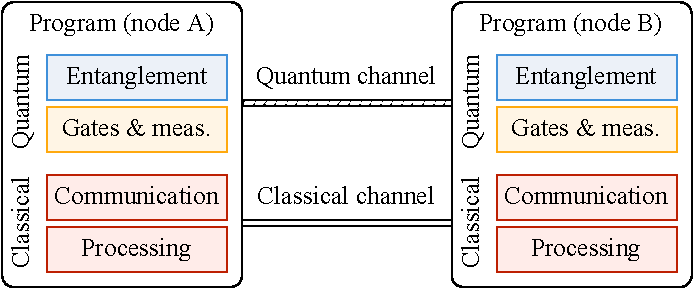
\includegraphics[width=0.6\linewidth]{figures/quantum-internet.pdf}
    \caption{
        A quantum networking application consists of separate programs running at two or more end
        nodes that communicate via classical message passing and quantum entanglement. Local
        operations include quantum operations (gates and measurements) as well as classical
        processing.
    }
    \label{fig:quantum-internet}
\end{figure}

Abstractly, a quantum networking application consists of multiple programs, each running on one of
the end nodes. The distinct programs only interact with one another by means of entanglement
generation and classical communication. This allows a programmer to realize security-sensitive
applications just as in the classical domain, but prohibits a global orchestration of the quantum
execution as one might do in quantum computing. The case of secure quantum computing in the
cloud~\cite{broadbent_2009_ubqc, childs_2005_secure_qc} is an example of a quantum networking
application, schematically depicted in \cref{fig:app-struct}. In blind quantum computing, a client
node wants to perform a computation on a remote server node, the latter being a powerful quantum
computer, without the server learning anything about the computation. Blind quantum computing
illustrates the need for a continuing interaction between the classical and quantum parts of the
execution, such as waiting for a message from a remote client before continuing the quantum
execution at the server. It also highlights the need for both classical and quantum state to be kept
alive, for example such that future quantum instructions can be executed depending on messages from
remote end nodes. This is in sharp contrast to quantum computing applications, where one can process
the entire quantum execution in a single batch.

\begin{figure}[t]
    \centering
    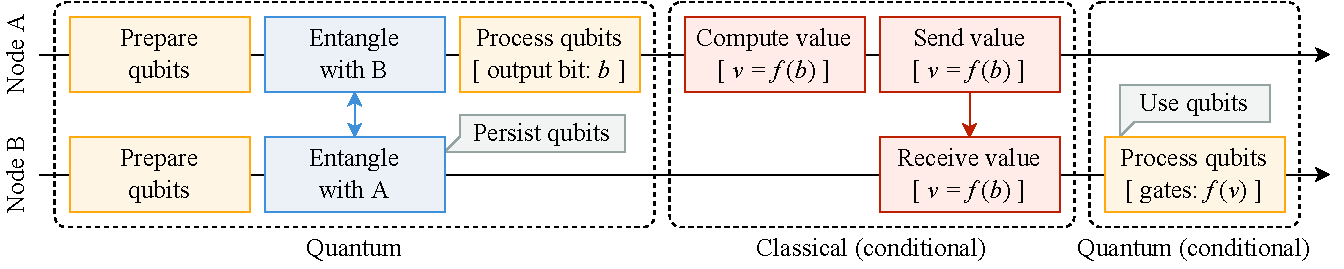
\includegraphics[width=\linewidth]{figures/app-struct.pdf}
    \caption{
        Structure of a typical quantum network application (blind quantum
        computation~\cite{broadbent_2009_ubqc, childs_2005_secure_qc}), which consists of
        interleaved quantum processing blocks and classical processing blocks. Quantum processing
        blocks include local quantum operations (gates and measurements, yellow boxes) and network
        operations (entanglement generation, blue boxes). The execution of some classical and
        quantum blocks might be conditional on classical and quantum data coming from previous
        blocks. Qubit states in quantum blocks may have to persist (``Persist qubits'') to be used
        in later quantum blocks (``Use qubits''), e.g. following the reception of classical messages
        from the remote node.
    }
    \label{fig:app-struct}
\end{figure}

Up to now, demonstrations of quantum networking beyond \acrshort{qkd} focused on hardware
realizations. Different types of end node quantum hardware have been realized, ranging from simple
photonic devices on which the only operation is a measurement~\cite{vallone_2015_satellite,
yin_2017_satellite}, to fully-fledged quantum processors with a network
interface~\cite{bernien_2013_heralded, humphreys_2018_delivery, pompili_2021_multinode,
moehring_2007_ion_traps, reiserer_2015_neutral_atoms}. The largest quantum network linking quantum
processors to date connects three nodes~\cite{pompili_2021_multinode} based on nitrogen-vacancy
centers in diamond (\acrshort{nv} centers) at the physical layer. Demonstrations of applications
beyond \acrshort{qkd} have been performed using several photonic
devices~\cite{barz_2012_demonstration, thalacker_2019_anonymous, bozzio_2020_coin,
ng_2012_noisystorage}. Central to all these demonstrations is that the software to control the
hardware was specific to the experiment setup, written to perform one single task (the experiment
itself) and programmed into low-level control devices. In fact, often applications were not even
actually fully realized towards a user, and instead they were meant to show that the hardware is in
principle good enough for that specific application~\cite{zhang_2022_diqkd,
liu_2022_photonic_diqkd}.

In order to advance quantum networks from a physics experiment to fully-fledged systems, we need a
combined software-hardware system that is built as a series of abstraction layers. These
abstractions should expose a simple interface for the user to write applications in high-level,
platform-independent software, and be able to interact with a variety of candidate platforms for
future quantum network hardware. When designing such a system, many challenges arise (refer to
\cref{sec:background:challenges} for details), which can be roughly classified into three areas.
First, there exist \emph{fundamental differences} between classical and quantum communication. A
example of this is the concept of heralded entanglement generation, which requires coordinated
actions by both nodes involved --- that is, the operations to produce entanglement need to be
scheduled at both nodes at the same time. Second, the \emph{technological limitations} of near-term
quantum devices impose stringent demands on the performance of such a system. One example is that
the same quantum device is used for processing as well as networking, which implies that local
operations cannot be scheduled independently of network operations --- which in turn depend on the
remote node. Finally, we remark that, unlike in the study of classical operating systems, which take
advantage of the existence of advanced computer architectures defining a specific interaction of
software and hardware, there exists \emph{no general low-level quantum processor architecture}.
Ideally, our system should be able to operate under the stringent constraints imposed by current
technological limitations, but should also not be tailored to near-term quantum devices only.

\section{Background}
\label{sec:background:background}

Here, we define some basic concepts of quantum networking hardware and performance metrics,
necessary to understand the remainder of this chapter and this thesis. We refer the reader to the
book \citetitle{nielsen_chuang_2002} by \textcite{nielsen_chuang_2002} for a general introduction to
quantum information, and to the article \citetitle{dahlberg_2019_egp} by
\textcite{dahlberg_2019_egp} for more information on quantum networking.

\paragraph{Quantum network nodes}

Generally speaking, a quantum network node is a quantum processor (or device) with an optical
interface for external communication (entanglement). The processor can perform operations on one or
more qubits. Local quantum operations range from simple qubit
measurements~\cite{vallone_2015_satellite, yin_2017_satellite} to universal quantum
computation~\cite{bernien_2013_heralded, humphreys_2018_delivery, pompili_2021_multinode,
moehring_2007_ion_traps, reiserer_2015_neutral_atoms}. Quantum networking operations allow certain
qubits to produce entanglement with a remote node. In practice, only some types of qubits are suited
for entanglement generation --- we refer to such qubits as \emph{communication qubits} --- and only
these qubits have an optical interface to the outside world. Other types of qubits --- referred to
as \emph{storage qubits} --- are instead more suited for storing quantum states for longer times (up
to seconds in some cases~\cite{abobeih_2018_one_sec, bradley_2019_one_min}). Often, storage qubits
can also be used to process quantum information directly. On some quantum devices instead, for
instance \acrlong{nv} centers in diamond (\acrshort{nv} centers), communication qubits are also the
main gateway for local quantum gates, meaning that most processing operations need to step though
these qubits, and thus their usage needs to be shared between local quantum computation and
entanglement generation. What operations can be performed on what types of qubits depends on the
specific quantum device. We remark that, at this stage of technological development, qubits, as well
as any quantum operations applied on them, are not perfect. In fact, their quality even depends on
the specific device sample being used.

\paragraph{Timing constraints}

Quantum devices are generally controlled using a variety of classical signal generators, depending
on the quantum device itself. For instance, in \acrshort{nv} centers, the quantum device is
controlled using microwave as well as laser pulses. The device-level control must satisfy hard
real-time constraints and timing precision --- nanosecond precision with sub-nanosecond jitter ---
and is realized using waveform generators, lasers, and custom electronics assisted by a dedicated
microcontroller. Entanglement generation between two nodes connected by an optical fiber also
requires the same scale of timing synchronization between the two devices~\cite{dahlberg_2019_egp,
pompili_2022_experimental}. The low-level control of other quantum platforms is realized
similarly~\cite{moehring_2007_ion_traps, reiserer_2015_neutral_atoms}. On top of those constraints,
qubits have a limited lifetime --- the states they hold must be processed before they become
invalid. On some devices, qubit lifetimes have been shown to exceed one
second~\cite{abobeih_2018_one_sec}. Nevertheless, the quality of a qubit state is not constant
throughout its lifetime, but it \emph{decoheres} (becomes worse) at a certain rate. Qubit lifetimes
and decoherence, however, are technological limitations, rather than fundamental ones, and are
expected to become more tractable in the future.

\paragraph{Performance metrics}

Next to standard classical performance metrics such as latency and throughput, the performance of
quantum networking applications hinges on the quality of the quantum execution too. In the quantum
networking domain, it is not generally an objective to eliminate all errors towards the application
level~\cite{dahlberg_2019_egp, vardoyan_2022_netarch}, and hence the performance of any operating
system for quantum network nodes would be measured by the execution quality, and by the trade-offs
with classical performance metrics~\cite{dahlberg_2019_egp, vardoyan_2022_netarch}. This quantum
quality is generally measured by the quantum \emph{fidelity} $F \in [0,1]$, where a higher value
corresponds to higher quality. For a quantum state, $F$ measures the quality with respect to an
ideal state. For a quantum gate or measurement, it measures the quality of execution, averaged over
all possible states that it could be applied to. For a specific application, $F$ can be translated
into its quantum performance.

\section{Challenges}
\label{sec:background:challenges}

Whilst the high-level goals for an operating system for quantum nodes mimic those of a classical
operating system, we face a number of general challenges inherent to (near-term) quantum network
nodes and network applications:
%
\begin{inlinelist}
    \item limited available qubits, which imposes strict limits on the processing, networking, and
          storage capabilities of networking nodes;
    \item limited qubit lifetimes, which imposes strict deadlines on how fast the data must be
          processed before it becomes useless;
    \item noisy operations, which implies that applying operations on qubits degrades the quality of
          the qubit states themselves;
    \item cross-node scheduling dependencies, meaning that the operations on one node cannot be
          scheduled independently of other nodes;
    \item interaction between classical and quantum parts of a program, which requires keeping
          quantum data alive in memory while waiting for an event to occur (e.g. a message from a
          remote network node).
\end{inlinelist}

The first three challenges are technological, that is, we expect the situation to improve with
further progress in quantum hardware development. Furthermore, to a certain extent, these issues are
common to quantum computing too, from which we can draw some inspiration for their solutions. The
fourth challenge is inherent to the nature of entanglement generation and to the physics of the
devices currently in use. Successful entanglement generation requires both nodes to execute a
network operation at the same moment in time. Moreover, at this stage of development, the same
quantum device functions as the processing unit and as the network device, and consequently local
quantum operations (such as measurements and gates) and network operations cannot be performed
simultaneously~\cite{vardoyan_2019_performance}. This limitation, however, could be mitigated by a
new quantum hardware architecture separating the devices~\cite{vardoyan_2022_netarch}. Finally, the
last challenge is a fundamental issue, as it applies to quantum network applications regardless of
technological progress. It is the last two points that fundamentally differentiate a quantum
networking node from a quantum computing system, and are the key driver for a \emph{networked}
quantum node operating system.

\begin{xstretch}
\printbibliography[heading=subbibintoc,title={References},notcategory=noprint]
\end{xstretch}

\chapter
 [Architecture of an Operating System for a Quantum Network Node]
 {Architecture of an\\Operating System for a\\Quantum Network Node}
\label{chp:arch}

\begin{abstract}
The end goal of an \acrfull{os} for quantum network nodes is to bridge the gap between user
applications --- written in high-level and platform-independent software --- and the underlying
quantum hardware, to which the user is agnostic. How can one design a control system that adheres to
this objective, while addressing the challenges that come with quantum networking? And what does an
example architecture of such a system look like? This chapter explores the cardinal design
considerations that should drive the design of an \acrshort{os} for quantum network nodes, and
proposes a proof-of-principle architecture for such an \acrshort{os}.
\end{abstract}

\noindent
\note{To be precise, this chapter is extracted from sections 3 (Design Considerations, but excluding
3.1) and 4 (\acrshort{qnodeos} Design) from the \acrshort{qnodeos} paper. There aren't any major
additions.}

\blfootnote{
    This chapter is based on the preprint \fullcite{delledonne_2023_qnodeos_noprint}. \note{Add
    proper link to arXiv when submitted}
}

\newpage

\lettrine{A}{n} \acrfull{os} is usually the cornerstone of a system's control software: it manages
and marshals access to physical resources, abstracts low-level hardware functionalities into
user-friendly services, and provides an interface to users to program and run applications on the
system. Our goal here is to apply basic principles from classical \acrshort{os} design literature to
our novel use case of programmable and scalable quantum networking nodes, and to hopefully create a
framework where the challenges outlined in \cref{chp:background} can be studied and addressed. We
thus investigate the general requirements that such a system should satisfy, illustrated with the
example of a quantum processor based on \acrfull{nv} centers in diamond. This provides a guideline
for future systems of this form. We also propose the first proof-of-principle architecture for an
\acrlong{os} for quantum network nodes, which we call \acrshort{qnodeos}. Our system's capabilities
include quantum memory management, scheduling different types of quantum operations on the device,
as well as an interface to different drivers addressing several possible quantum hardware
architectures. On the quantum networking front, \acrshort{qnodeos} adopts the quantum network stack
and protocols proposed by \textcite{dahlberg_2019_egp} and by \textcite{kozlowski_2020_qnp}.

\section{General Design Considerations}
\label{sec:arch:considerations}

We assume that the operating system builds upon a quantum hardware system capable of the execution
of \emph{physical instructions} addressing specific qubits on the quantum chip. These physical
instructions may be dependent on the type of quantum hardware (e.g. \acrshort{nv} in diamond, or ion
traps), and include instructions for initializing and measuring qubits on the chip, moving the state
of a qubit to another location in the quantum memory, performing quantum gates, as well as to make
attempts at entanglement generation at the physical layer~\cite{pompili_2022_experimental}. The
quantum hardware furthermore exposes the capabilities of the quantum chip: (1) the number of qubits
(2) the type of each qubit (3) the memory lifetime of the qubits (4) the physical instructions that
can be performed on on the qubit(s) and (5) the average quality of these instructions
(\cref{chp:background}). We emphasize that, unlike in classical computing, there is currently no
established low-level microarchitecture that defines the line between (quantum) hardware and
software upon which such an operating system would be built. We nevertheless expect that almost all
of the below would be functions taken on by any operating system, some of which could possibly be
shifted to control hardware in the future.

Each node in the network runs its own independent quantum network operating system. Nodes may
interact with each other using both classical message passing as well as entanglement generation.
The goal of the combined system is to execute quantum network applications, which themselves consist
of separate programs running on the operating system(s) of two (or more) network nodes. Such
programs generally also communicate via classical message passing and entanglement generation. Each
program itself consists of both classical and quantum blocks of code, where the quantum blocks of
code may contain low-level classical logic (specifically, branching on classical variables and
loops). Classical blocks of code may depend on quantum ones via classical variables generated during
the quantum execution (measurement results, notification of entanglement generation, and information
on the state of the quantum system such as the availability of qubits). Similarly, quantum blocks
may depend on variables set by the classical blocks, such as messages received from remote network
nodes. Finally, quantum blocks may themselves depend on other quantum blocks via qubits in the
quantum memory. It is the responsibility of the programmer or compiler to identify what is a
classical and what is a quantum block. Similarly, we assume that (potentially fine-grained)
deadlines or priorities in the execution are determined by the programmer (or compiler) using the
knowledge of the exposed capabilities of the quantum hardware system (e.g. memory lifetimes).
Determining precise deadlines (e.g. when too much time has elapsed for the qubits to be useful) is
in general a computationally expensive procedure, sometimes estimated in practice by a repeated
simulation of the execution. We remark that there is no way in quantum mechanics to measure the
current quality of a qubit or operation during the ongoing execution, and such qualities are
determined by performing estimates independently of the program execution itself. Of course, the
operating system could itself engage in such estimates when idling in order to update its knowledge
of the capabilities of the quantum hardware.

\section{Key \acrshort{os} Components}
\label{sec:arch:components}

We now describe the essential components we envision any operating system for quantum network nodes
to have.

\subsection{Memory Management Unit}

Executing quantum network applications demands a continuing interaction between the classical and
quantum parts of the execution, including keeping qubits alive in memory to take further actions
depending on messages from remote network nodes. We thus require persistent memory management
capabilities. This may be taken up by a \emph{\acrlong{qmmu}} (\acrshort{qmmu}). A \acrshort{qmmu}
has knowledge of the physical qubits available on the underlying quantum hardware, and may keep any
other information about said qubits, such as the qubit type (communication or storage qubit) and
qubit lifetime. A \acrshort{qmmu} allows physical qubits to be assigned to different applications or
to the operating system itself, and may allow a transfer of ownership of the qubits from one owner
to another. A \acrshort{qmmu} may also provide abstractions familiar to classical computing such as
a virtual address space, where the applications refer to virtual qubit addresses that are then
translated to physical qubit addresses. This avoids the situation in which physical qubit addresses
must be bound at compile time, particularly limiting when allowing multiple applications to
concurrently run on the same node. Advanced forms of a \acrshort{qmmu} may also cater to the
limitations of near term quantum devices, by matching memory lifetime requirements specified by the
application code to the capabilities of the underlying qubits, as well their topology (i.e. taking
into account which two qubits allow two-qubit gates to be performed on them directly). While one
cannot measure the decoherence of a qubit during a general program execution on the quantum level,
the \acrshort{qmmu} could also take into account additional information from the classical control
system to signal to the application that a qubit has become invalid.

\subsection{Quantum Network Stack}

The \acrshort{os} should include the capability for quantum communication with remote nodes in the
network, typically the generation of entanglement. We thus assume that the \acrshort{os} realizes a
quantum network stack that can be relied upon to enable entanglement generation, where we refer to
Ref.~\cite{dahlberg_2019_egp} for design considerations of quantum network stacks themselves. The
network stack allows an application to request a certain number or rate of entangled pairs to be
produced with remote nodes with a specified quality (i.e. fidelity) of entanglement. The stack is
responsible for ensuring the delivery of the entanglement. One possible quantum network stack can be
found in Ref.~\cite{dahlberg_2019_egp} including the first link layer protocol now realized on
quantum hardware~\cite{pompili_2022_experimental} (as described in \cref{chp:netstack}), and a
network layer protocol (as proposed in Ref.~\cite{kozlowski_2020_qnp}).

To successfully produce entanglement, the network stack needs access to a communication qubit,
resulting in two requirements for the rest of the system:
%
\begin{inlinelist}
    \item A scheduler (see below) should take into account that generating entanglement at the
          physical layer between two nodes directly connected by a physical communication medium
          requires that the two nodes apply a series of physical operations with very precise timing
          synchronization between them (nanosecond precision with sub-nanosecond jitter). Therefore,
          entanglement generation across a link with an adjacent node must always be scheduled in a
          synchronized manner between the two adjacent neighbors. Similarly, due to limited memory
          lifetimes, generating entanglement with the help of an intermediary node at the network
          layer~\cite{kozlowski_2020_qnp} requires specific operations (entanglement swapping) to be
          scheduled at all three nodes within a time window allowed by the memory lifetimes.
    \item On some quantum hardware systems (e.g. \acrshort{nv} in diamond), the communication qubit
          is in general needed to enable the execution of quantum gates on and in-between storage
          qubits. This has implications both on the scheduler (local instructions cannot be
          scheduled concurrently to networked ones), as well as on the \acrshort{qmmu}, which needs
          to allow qubit ownership transfer between applications and the network stack. A typical
          use case of such ownership transfer would occur when the network stack claims the
          communication qubit for entanglement generation, and then yields it to an application.
\end{inlinelist}

\subsection{Scheduler}

In order to maximize the usage of resources, we envision the \acrshort{os} to include a scheduler.
This may be a single scheduler, or more likely several schedulers that address scheduling at
different levels. In general, we may consider scheduling at the level of applications, at the level
of blocks of quantum code, and at the level of instructions, each level not being independent of one
another.

\paragraph{General considerations}

A scheduler for quantum network nodes should be capable of managing the limited physical resources
to achieve the desired performance. The performance of any form of scheduling method in the quantum
domain is assessed not only by existing classical metrics --- like throughput and latency --- but
also by quantum metrics (see \cref{chp:background}). At the level of the application, latency can be
measured in terms of the success probability of the quantum network application. At the level of an
operation (or a block of operations) it may be measured by the quality (fidelity) of the quantum
states and operations performed. We remind that due to limited memory lifetimes, delays have always
a direct impact on the quantum performance, resulting in general in trade-offs between classical and
quantum performance metrics when assessing any scheduler.

Practically, the scheduler in question should allocate the underlying physical resources --- most
importantly, the qubits --- based on a set of well-defined constraints, the fundamental ones being:
%
\begin{inlinelist}
    \item \emph{Synchronized network schedule}: due to the bilateral nature of entanglement, each
          node will have its quantum networking activity synchronized with its neighbors, meaning
          that a missed synchronization window on one node results in a waste of resources on remote
          nodes too.
    \item \emph{Local quantum computation}: in addition to quantum networking, a node's resources
          must also be reserved for local quantum gates, which are integral parts of quantum
          networking applications.
    \item \emph{Inter-block dependencies}: quantum and classical processing blocks of an application
          may depend on results originating from other blocks, and thus cannot be scheduled
          independently.
    \item \emph{Multitasking}: for a node to be shared by multiple users, the scheduler should not
          allocate all the available resources to a single application indefinitely, and instead it
          should be aware of the presence of multiple applications and multiple users.
\end{inlinelist}

Additionally, scheduling at any level could optionally process another set of input variables, where
we generally assume that the programmer or compiler provide aggregate advice based on these input
variables to the \acrshort{os}:
%
\begin{inlinelist}
    \item \emph{Duration of operations}: local quantum operations typically take a fixed amount of
          time and always succeed. Entanglement, on the other hand, is a probabilistic process, and
          generating an entangled pair can take an indefinite (and large) number of attempts.
          Scheduling decisions may factor this in to yield better performance.
    \item \emph{Decoherence}: as already stated, the fidelity of a quantum state stored in a qubit
          is not constant, and it also degrades due to physical noise induced by other qubits and by
          operations applied on such qubits. An advanced scheduler could use knowledge of qubit
          lifetimes and elapsed time to dynamically re-prioritize application demands based on the
          advice of the compiler.
\end{inlinelist}

\paragraph{Scheduling of applications}

In an \acrshort{os} allowing the execution of concurrent quantum network applications, the task of
an application-level scheduler would be to decide which application to schedule next. We remark that
a programmer (or compiler) aware of the underlying capabilities of the hardware system (e.g. memory
lifetimes) can provide advice in the form of a deadline by which the network application must have
completed in order to be successful. To allow for potentially time-consuming classical pre- and
post-processing, it is natural to apply such deadlines not for the entirety of the application, but
for the period between initializing the qubits and terminating the quantum part of the execution.
This suggests in general using real-time schedulers for quantum network applications, taking
inspiration from the extensive work on this topic in classical systems (see e.g.
Ref.~\cite{liu_1973_scheduling}). While outside the scope of this work, we remark that this type of
scheduling offers to inspire interesting new work in a form of ``quantum soft-real time''
scheduling, where deadlines may occasionally be missed at the expense of reduced application
performance (success probability), to maximize the overall performance of the system in which
applications are typically executed repeatedly. A benchmark for the quantum performance of any
application-level scheduler is the quality of the quantum execution when the entire system (all
nodes) are reserved for only one application at the time.

\paragraph{Scheduling of quantum blocks}

Scheduling can also (additionally) be performed on the level of quantum blocks of code. This can in
principle also take the form of a (soft) real-time scheduler that schedules blocks of the currently
running application, or schedule blocks of several applications (potentially independently of any
application level scheduling) depending on the availability of resources on the quantum hardware
system. This form of scheduling may be appealing for efficiency reasons, depending on where what
parts of the operating system are executed, where some parts are closer to the underlying hardware
system than others (see e.g. \cref{sec:arch:design}).

\paragraph{Scheduling of operations}

Finally, scheduling can be performed at two levels of operations: First, one can consider the
problem of scheduling local versus networked instructions, where one simple way of realizing a
schedule that respects the constraints inherent in such a schedule (see above) is presented in
\cref{sec:arch:design}. Second, one can consider scheduling any form of operation on the underlying
quantum processor. While our current realization of \acrshort{qnodeos} achieves this by populating
an instruction queue in software, we envision that this form of scheduling would later be moved from
\acrshort{qnodeos} to a hardware module in a microarchitecture for quantum networking nodes, as for
instance in the work by \textcite{fu_2017_microarch}.

\section{\acrshort{qnodeos} Design}
\label{sec:arch:design}

\acrshort{qnodeos} is an operating system for quantum network nodes, designed to address the
challenges described in \cref{chp:background}. It includes all the identified key components, plus
some additional convenience abstraction layers. The current design of \acrshort{qnodeos} is
considered \emph{best-effort} --- it is meant to explore the main design aspects of an operating
system for quantum networks, and to provide a minimum working system.

\subsection{Full Stack of a Quantum Network Node}

As described in \cref{chp:background} and illustrated in \cref{fig:app-struct}, a quantum network
application consists of programs running on different end nodes, composed of blocks of quantum code
and blocks of fully-classical code. In fact, quantum code blocks may also contain simple classical
logic --- like simple arithmetic and branching instructions --- used for flow control. These blocks
do not have any dependencies on data originating from other nodes. Fully-classical code blocks ---
which include local processing and communication with other end nodes --- mainly produce input data
for the next quantum code blocks. That is, a classical code block typically precedes a quantum code
block whose instructions depend on external data coming from a remote end node. In our system,
quantum code blocks expressed in \emph{NetQASM}~\cite{dahlberg_2022_netqasm}. NetQASM is an
open-source \acrfull{sdk} and instruction set for quantum applications~\cite{netqasm_sdk}. The
NetQASM \acrshort{sdk} compiles a quantum network application, written in Python, into a series of
classical and quantum code blocks. The instruction set used for the quantum code blocks is similar
to other QASM languages~\cite{cross_2017_qasm, khammassi_2018_cqasm, fu_2019_eqasm}, but it is
extended to include instructions for quantum networking. NetQASM is not a strict requirement of
\acrshort{qnodeos}, but it does impose certain conventions (described in
Ref.~\cite{dahlberg_2022_netqasm}) on a particular implementation of the system.

In principle, classical and quantum code blocks can be run on a single system, provided that this
has a connection to the quantum device to execute the actual quantum instructions. However, in the
interest of a simpler implementation, where each system has a scoped responsibility, we opted to map
classical and quantum blocks onto two distinct environments. Classical blocks are run on a system
that features a fully-fledged \acrshort{os} (like Linux), with access to high level programming
languages (like C++ and Python) and libraries. Quantum blocks are delegated to the
\emph{\acrlong{qnpu}} (\acrshort{qnpu}), which is a system capable of interpreting quantum code
blocks and managing the resources of a quantum device. In our design, a quantum network application
starts on the general-purpose \acrshort{os} --- that we call the \emph{host} --- which runs
classical code blocks internally, and offloads quantum code blocks to the \acrshort{qnpu}.
\acrshort{qnodeos} is the topmost component of the \acrshort{qnpu}. It runs the quantum code blocks,
relying on the underlying quantum device --- denoted as \emph{\acrshort{qdevice}} --- to execute the
actual quantum operations.

The architecture of a quantum network node is depicted in \cref{fig:quantum-node}. An alternative
architecture could merge host and \acrshort{qnodeos} into the same system, potentially enabling some
performance optimizations, at the cost of a higher system complexity. We also note that the host,
\acrshort{qnodeos} and the classical control modules of the \acrshort{qdevice} can be deployed on
distinct physical devices, or combined in some way.

\begin{figure}[t]
    \centering
    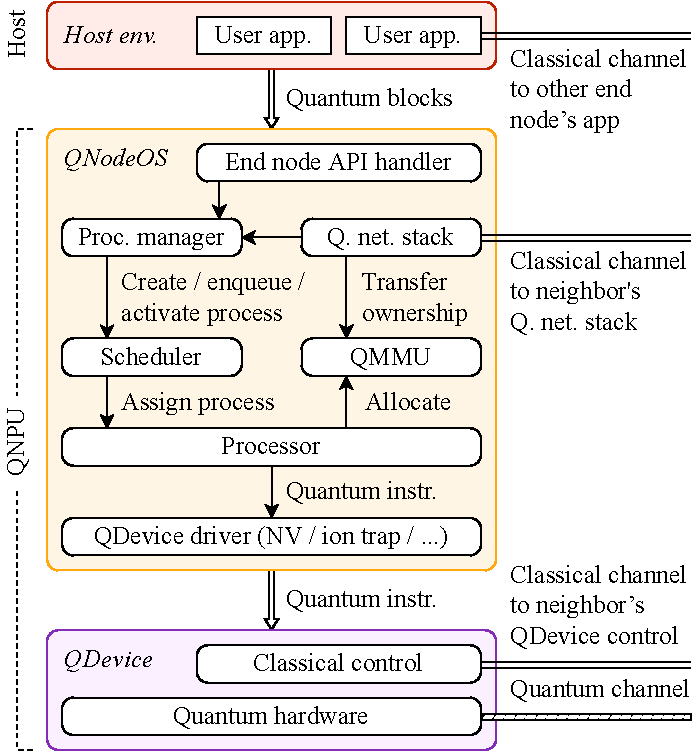
\includegraphics[width=0.6\linewidth]{figures/quantum-node.pdf}
    \caption{
        Full-stack architecture of a quantum network node. User applications start in the host
        environment, which runs classical code blocks and offloads quantum code blocks to the
        \acrshort{qnpu}. \acrshort{qnodeos}, lying at the top of the \acrshort{qnpu}, processes
        quantum code blocks and invokes the quantum device (\acrshort{qdevice}) to run the actual
        quantum instructions. \acrshort{qnodeos} consists of an end-node \acrshort{api} handler, a
        quantum network stack (Q. net. stack), a process manager (Proc. manager), a quantum memory
        management unit (\acrshort{qmmu}), a scheduler, a processor, and a \acrshort{qdevice} driver
        to communicate with the \acrshort{qdevice} itself. The host shares a classical communication
        channel with other end nodes' hosts for application data. \acrshort{qnodeos} shares a
        classical channel with its neighbors. The \acrshort{qdevice} shares a classical channel for
        coordination and a quantum channel for entanglement with its neighbors.
    }
    \label{fig:quantum-node}
\end{figure}

\subsection{Processes}

A quantum network application starts on the host --- there, the host environment compiles it into
classical and quantum code blocks, and creates a new process associated with the application. The
host then registers the application with \acrshort{qnodeos} (through \acrshort{qnodeos}'s end-node
\acrshort{api}), which, in turn, creates its own process associated with the registered application.
The process on the host is a standard \acrshort{os} process, which executes the classical code
blocks and interacts with the counterpart process on \acrshort{qnodeos} (by means of a shared
memory, as defined in NetQASM~\cite{dahlberg_2022_netqasm}). On \acrshort{qnodeos}, a process
encapsulates the execution of quantum code blocks of an application with associated context
information, such as process owner, ID, process state and priority.

The execution time of an application is typically dominated by that of quantum blocks, as
entanglement generation is a time-consuming operation, and its duration grows exponentially with the
distance between the nodes. For this reason, in this work we focus on the scheduling of quantum
blocks only, and thus we only discuss \acrshort{qnodeos} processes from this point onward. Again,
this does not exclude that, in a future iteration of the design, host and \acrshort{qnodeos} could
be merged into one system, and therefore classical and quantum blocks would be scheduled jointly.

\paragraph{\acrshort{qnodeos} user processes}

\acrshort{qnodeos} allocates a new \emph{user process} to each quantum network application
registered by the host. A user process becomes active (ready to be scheduled) as soon as
\acrshort{qnodeos} receives a quantum code block from the host. Multiple user processes --- relative
to different host applications --- can be concurrently active on \acrshort{qnodeos}, but only one
can be running at any time. A running user process executes its quantum code block directly, except
for entanglement requests, which are instead submitted to the quantum network stack and executed
asynchronously.

\paragraph{\acrshort{qnodeos} network process}

\acrshort{qnodeos} also defines \emph{kernel processes}, which are similar to user processes, but
are created by default (on boot) and have different priority values. Currently, the only existing
kernel process is the \emph{network process}. The network process, owned by the quantum network
stack, handles entanglement requests submitted by user processes, coordinates entanglement
generation with the rest of the network, and eventually returns entangled qubits to user processes.
The activation of the network process is dictated by a network-wide entanglement generation
schedule. Such a schedule defines when a particular entanglement generation request can be
processed, and therefore it has intersecting entries on adjacent nodes (given that entanglement is a
two-party process). The schedule can be computed by a centralized network
controller~\cite{skrzypczyk_2021_arch} or by a distributed protocol~\cite{dahlberg_2019_egp}. In our
design, the network process follows a \emph{time-division multiple access schedule}, computed by a
centralized network controller (as originally proposed by \textcite{skrzypczyk_2021_arch}) and
installed on each \acrshort{qnodeos} node.

\paragraph{\acrshort{qnodeos} process states}

A \acrshort{qnodeos} process can be in any of the following states:
%
\begin{inlinelist}
    \item \emph{idle}: when it exists but it is not active;
    \item \emph{ready}: when it is active and ready to issue instructions;
    \item \emph{running}: when it is running on \acrshort{qnodeos};
    \item \emph{waiting}: when it is waiting for some event to occur.
\end{inlinelist}
User processes enter the waiting state when they need one or more entangled pairs to proceed, and
become ready again once all the requested pairs are delivered by the network process.

\paragraph{Inter-process communication}

At the moment, \acrshort{qnodeos} does not allow for any explicit inter-process communication. The
only indirect primitive available to processes to interact with one another is \emph{qubit ownership
transfer}, used when a process produces a qubit state which is to be consumed by another process. In
particular, the network process transfers ownership of the entangled qubits that it produces to the
process which requested them.

\paragraph{Process concurrency}

The strict separation between local quantum processing and quantum networking is a key design
decision in \acrshort{qnodeos}, as it helps us address the scheduling challenge described in
\cref{chp:background}. A user process can continue executing local instructions even after it has
requested entanglement. Conversely, networking instructions can execute asynchronously of local
quantum instructions. This is rather important in a quantum network, since entanglement generation
must be synchronized with the neighboring node (and possibly the rest of the
network~\cite{skrzypczyk_2021_arch}). Additionally, separating user applications into user processes
also allows \acrshort{qnodeos} to schedule several applications \emph{concurrently}.

\begin{figure}[t]
    \centering
    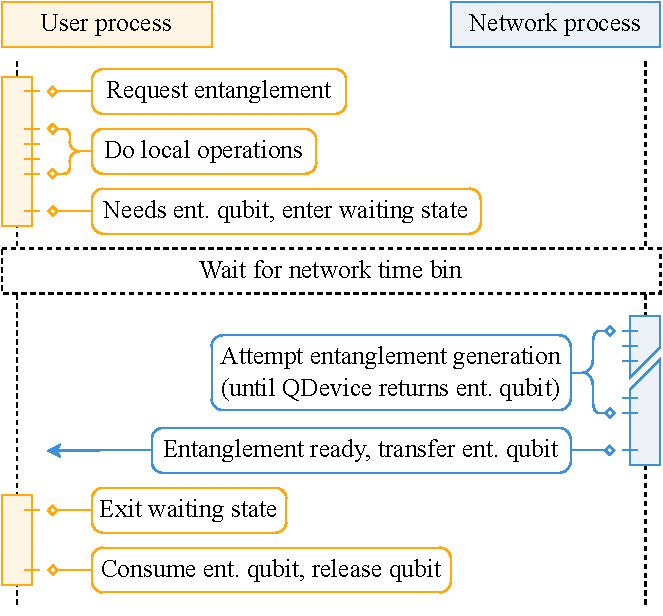
\includegraphics[width=0.6\linewidth]{figures/process-flow.pdf}
    \caption{
        Flow of execution between a user process requesting entanglement and the network process
        responsible for generating entanglement. The user process starts by issuing an asynchronous
        entanglement request. Once issued, it is free to continue with other local operations or
        classical processing. Once it reaches a point in its execution where entanglement is
        required the process enters the waiting state. The network process is then scheduled once
        the appropriate time bin starts, as determined by the network schedule. Once it is running,
        the network process attempts entanglement generation until entanglement success (or until a
        set timeout). The entangled qubit is then transferred to the user process. This unblocks the
        process which consumes the entanglement and releases the qubit.
    }
    \label{fig:process-flow}
\end{figure}

\paragraph{Process flow}

\Cref{fig:process-flow} illustrates the typical control flow between a user process and the network
process. User processes are free to execute any non-networked instructions independently of the
network process and other user processes. Once the application reaches a point in its execution
where an entangled qubit is required, the process enters the waiting state and is flagged as waiting
for entanglement. When the network process is scheduled, it issues network instructions and
generates entanglement as requested by the user process. Once an entangled pair is generated by the
network process, the qubit is handed over to the waiting user process. When all the entangled pairs
that the user process was waiting for are delivered, the user process becomes ready and can start
running again.

\subsection{Process Scheduling}

As previously mentioned, we focus our attention on the quantum blocks of an application, and thus we
only discuss the scheduling of \acrshort{qnodeos} processes. At present, the \acrshort{qnodeos}
scheduler does not give any guarantees on when a process is scheduled --- for that, one would need
to define concrete real-time constraints to feed to the scheduler. Instead, the current version of
\acrshort{qnodeos} implements a best-effort scheduler, which selects processes on the basis of their
priority, and does not allow preemption.

\paragraph{Priority scheduling}

\acrshort{qnodeos} schedules ready processes using a \emph{priority-based} algorithm. In particular,
the network process is assigned the highest priority, and is given precedence whenever the network
schedule activates it~\cite{skrzypczyk_2021_arch}. Prioritizing entanglement generation over local
operations is key for a node to be able to fulfill its networking duty, and to avoid peer nodes to
waste their resources.

\paragraph{No preemption}

To avoid context switching overhead, potentially leading to degraded fidelity, the
\acrshort{qnodeos} scheduler is \emph{cooperative}. That is, once a process is scheduled, it gets to
run until it either completes all of its instructions or it blocks waiting for entanglement.
Allowing process preemption would need a definition of critical section and could potentially impact
the quality of the affected qubit states.

\subsection{\acrshort{qnodeos} Architecture}

\Cref{fig:quantum-node} illustrates the internals of \acrshort{qnodeos}, and outlines the
interactions with the rest of the components of a quantum network node. At its top,
\acrshort{qnodeos} implements an \emph{end-node \acrshort{api} handler} to process requests from the
host. Internally, \acrshort{qnodeos} features a \emph{quantum network stack}, a \emph{process
manager}, a \emph{process scheduler}, a \emph{quantum memory management unit} (\acrshort{qmmu}), and
an \emph{instruction processor}. Actual quantum instructions are offloaded to the underlying quantum
device (\acrshort{qdevice}) through the \emph{\acrshort{qdevice} driver}.

We note that \acrshort{qnodeos} itself is an entirely classical system that interacts with the
quantum hardware (the \acrshort{qdevice}). At the moment, our implementation of \acrshort{qnodeos}
is fully software, including the instruction processor. In general, the system may be implemented
entirely in software running on a classical \acrshort{cpu}, or parts of its functionality may be
implemented in classical hardware (e.g.~\acrshort{fpga} or \acrshort{asic}).

\paragraph{End-node \acrshort{api}}

Each user application is registered on \acrshort{qnodeos} by the host through the end-node
\acrshort{api}. Using the same \acrshort{api}, the host can then send quantum code blocks and
receive their results (like measurement outcomes and entanglement generation information). Upon
registration of an application, \acrshort{qnodeos} allocates a new user process. Upon reception of a
quantum code block, the related user process is activated and made eligible for scheduling.

\paragraph{Process manager, scheduler, processor}

The \acrshort{qnodeos} process manager keeps track of existing user and kernel processes and their
execution context. Upon activation, processes are added to a scheduling queue. When selected by the
scheduler, a process is assigned to the \acrshort{qnodeos} processor, which
%
\begin{inlinelist}
    \item executes classical control-flow instructions directly,
    \item offloads local quantum computation to the \acrshort{qdevice}, and
    \item registers entanglement requests with the quantum network stack.
\end{inlinelist}

\paragraph{Quantum network stack}

The role of the quantum network stack in \acrshort{qnodeos} is to abstract the unreliable
entanglement attempts that the \acrshort{qdevice} offers into a robust, multi-node network service.
The network stack can handle entanglement generation requests which specify a number of parameters
--- including source and destination, desired fidelity, and number of entangled pairs --- and
returns the entangled pair(s) described by an identifier and the generated Bell state. The quantum
network stack owns the network process, whose activation is dictated by a network-wide entanglement
schedule. The quantum network stack in \acrshort{qnodeos} is based on the model outlined by
\textcite{dahlberg_2019_egp}, and features a \emph{link layer protocol} --- presented in the same
work, and recently evaluated on hardware~\cite{pompili_2022_experimental} (\cref{chp:netstack}) ---
and a \emph{network layer protocol} --- as designed by \textcite{kozlowski_2020_qnp}.

\paragraph{Quantum memory management unit}

\acrshort{qnodeos}'s \acrshort{qmmu} implements basic memory management functionality: \emph{virtual
address spaces} and \emph{qubit ownership transfer}. A virtual quantum memory address space is akin
to a classical virtual address space, but it isolates the qubit address spaces of \acrshort{qnodeos}
processes. Ownership transfer is an indirect type of \acrfull{ipc} mechanism for passing quantum
data between processes. Since quantum states cannot be copied due to the no-cloning theorem, this is
the only valid \acrshort{ipc} for passing quantum data between address spaces. Ownership transfer is
only logical --- only the data's owner is updated --- rather than it being a physical move of
quantum data in the memory. This way we can avoid issuing a \acrshort{qdevice} instruction which
would cause degradation in fidelity due to hardware imperfections and additional processing time.
The current \acrshort{qmmu} is rather simple due to the fact that our current quantum nodes have
only have a few qubits each. Features like decoherence tracking and topology-based allocation can be
part of a later version of the \acrshort{qmmu}.

\printbibliography[heading=subbibintoc,title={References},notcategory=noprint]

\chapter{Entanglement Generation With a Quantum Networking Stack}
\label{chp:netstack}

\begin{abstract}
Entanglement generation has already been demonstrated a few times by now, at various node-to-node
distances, on several quantum physical platforms, and mostly on small-scale quantum networks.
Scaling current quantum communication demonstrations to a large-scale quantum network will require
not only advancements in quantum hardware capabilities, but also robust control of such devices to
bridge the gap in user demand. Moreover, the abstraction of tasks and services offered by the
quantum network should enable platform-independent applications to be executed without the knowledge
of the underlying physical implementation. In this chapter, we experimentally demonstrate
entanglement generation through \acrshort{qnodeos} and its quantum networking stack.
The link layer abstracts the physical-layer entanglement attempts into a robust,
platform-independent entanglement delivery service. The system is used to run full state
tomography of the delivered entangled states, as well as preparation of a remote qubit state on
a server by its client. Our results mark a clear transition from physics experiments to quantum
communication systems, which will enable the development and testing of components of future
quantum networks.
\end{abstract}

\noindent
\note{This chapter is extracted from the npj paper. No major additions.}

\blfootnote{
    This chapter is based on the article: \fullcite{pompili_2022_experimental_noprint}.
}

\newpage

\lettrine{N}{ear-term} quantum networks have already yielded successful experimental results towards
a future quantum internet. Fundamental primitives for entanglement-based quantum networks have been
demonstrated across several physical platforms, including trapped
ions~\cite{moehring_2007_ion_traps, stephenson_2020_highrate}, neutral
atoms~\cite{ritter_2012_elementary, hofmann_2012_heralded}, diamond color
centers~\cite{bernien_2013_heralded, kalb_2017_entanglement, humphreys_2018_delivery,
pompili_2021_multinode}, and quantum dots~\cite{delteil_2016_generation, stockill_2017_phasetuned}.
To scale up such physics experiments to intermediate-scale quantum networks, researchers have been
investigating how to enclose the complex nature of quantum entanglement generation into more robust
abstractions~\cite{aparicio_2011_protocol, dahlberg_2019_egp, pirker_2019_quantum,
kozlowski_2020_qnp, aguado_2020_enabling, kozlowski_2020_p4, alshowkan_2021_reconfigurable}.

A common way to facilitate the scalability of complex systems is to break down their architecture
into a stack of layers. Each layer in such a stack is characterized by a specific service that it
provides to the high layers, reducing complexity for the higher layers, which can subsequently rely
on this service. Moreover, the higher layers need no knowledge of the specific protocol and physical
realization that a lower layer uses to realize the specified service. An example from classical
networking is the \acrshort{tcpip} stack used on the present day internet. In this stack, the link
layer enables reliable transmission of data between two network nodes that are directly connected by
an unreliable physical medium such as fiber or radio. Higher layers can rely on errors being
detected by the link layer, and are agnostic about whether the underlying link layer protocol is
Ethernet or Wi-Fi.

Several network stacks have been proposed for quantum network nodes~\cite{dahlberg_2019_egp,
pirker_2019_quantum, kozlowski_2020_qnp}, like the one depicted in \cref{fig:netstack}. These draw
inspiration from classical architectures like the \acrshort{tcpip} stack or the more generic
\acrfull{osi} model. Specifically, the functional allocation of the stack proposed in
Ref.~\cite{dahlberg_2019_egp} conceptually mirrors the \acrshort{tcpip} stack in that the link layer
ensures reliable (quantum) communication between adjacent nodes, and the network layer extends this
service to nodes not directly connected by a physical medium themselves. We emphasize that of course
no quantum data is passed up and down the layers of the stack, but only qubit metadata. Very
intuitively, such metadata is similar to passing only references to an address in a physical memory
up and down the stack (similar to what happens in many implementations of the \acrshort{tcpip} stack
in practice), while in the classical case data may of course also be copied up and down layers.

We also note that the quantum internet, and the associated quantum network stack, do not aim to
replace the classical internet --- they will likely coexist, as the quantum internet cannot operate
without classical communication in practice. In addition to classical information used to facilitate
entanglement generation, we also expect classical communication at the level of the quantum
application itself (e.g.~quantum key distribution), which would for practical reasons be performed
using the classical internet. Finally, in a quantum network, classical communication could also be
used to realize controllers like those at the core of \acrfull{sdn}~\cite{ferguson_2021_orion} to
distribute information for resource scheduling and quality of service~\cite{skrzypczyk_2021_arch}.
The proposed quantum network stack architecture, along with proposals for resource scheduling and
routing techniques (e.g.~\cite{van_meter_2013_path, caleffi_2017_optimal,
gyongyosi_2018_decentralized, pant_2019_routing, chakraborty_2019_distributed, shi_2020_concurrent,
chakraborty_2020_entanglement, skrzypczyk_2021_arch}), pave the way for larger-scale quantum
networks.

In this work we experimentally demonstrate a link layer protocol for entanglement-based quantum
networks. The link layer abstracts the generation of entangled states between two physically
separated solid-state qubits into a robust and platform-independent service. An application can
request entangled states from the link layer and then, in addition, apply local quantum operations
on the entangled qubits in real-time. Using the link layer, we perform full state tomography of the
generated states and achieve remote state preparation --- a building block for blind quantum
computation --- as well as measuring the latency of the entanglement generation service.

To evaluate correct operation and performance of our system, we measure
\begin{inlinelist}
    \item the fidelity of the generated states and
    \item the latency incurred by link layer and physical layer when generating entangled pairs.
\end{inlinelist}
For both fidelity and latency, we find that our system performs with marginal overhead with respect
to previous non-platform-independent experiments. We also identify the sources of the additional
overhead incurred, and propose improvements for future realizations.

\begin{figure}[t]
    \centering
    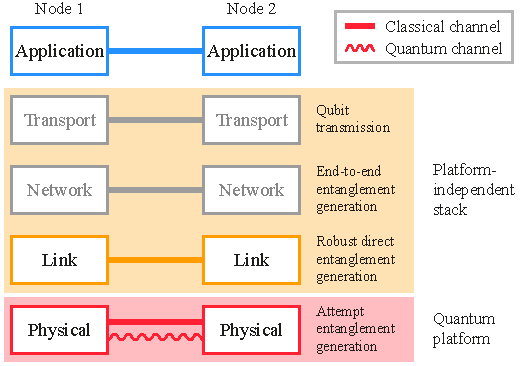
\includegraphics[width=0.6\linewidth]{figures/netstack.pdf}
    \caption{
        Quantum network stack architecture. At the bottom of the stack, the physical layer (red),
        which is highly quantum platform-dependent, is tasked with attempting entanglement
        generation. The link layer (yellow) uses the functionality provided by the physical layer to
        provide a platform-independent and robust entanglement generation service between
        neighboring nodes to the higher layers. Network and transport layer (not implemented in this
        work, grayed out) will support end-to-end connectivity and qubit transmission. Applications
        (blue) use the services offered by the stack to perform quantum networking tasks. Based on
        Ref.~\cite{dahlberg_2019_egp}.
    }
    \label{fig:netstack}
\end{figure}

\section{Quantum Link Layer Protocol}
\label{sec:netstack:link}

Remote entanglement generation constitutes a fundamental building block of quantum networking.
However, for a user to be able to integrate it into more complex quantum networking applications and
protocols, the entanglement generation service must also be:
%
\begin{inlinelist}
    \item robust, meaning that the user should not have to deal with entanglement failures and
          retries, and that an entanglement request should result in the delivery of an entangled
          pair;
    \item quantum platform-independent, in order for the user to be able to request entanglement
          without having to understand the inner workings of the underlying physical implementation;
    \item on-demand, such that the user can request and consume entanglement as part of a larger
          quantum communication application.
\end{inlinelist}
Robust, platform-independent, on-demand entanglement generation must figure as one of the basic
services offered by a system running on a quantum network node. In other words, establishing a
reliable quantum link between two directly connected nodes is the task of the first layer above the
physical layer in a quantum networking protocol stack, as portrayed in \cref{fig:netstack}.
Following the \acrshort{tcpip} stack nomenclature, we refer to this layer as the \emph{link layer}.
We remark that, in the framework of a multi-node network, a quantum network stack should also
feature a \emph{network layer} (called \emph{internet layer} in the \acrshort{tcpip} model) to
establish links between non-adjacent nodes, and optionally a \emph{transport layer} to encapsulate
qubit transmission into a service~\cite{dahlberg_2019_egp, kozlowski_2020_qnp, pirker_2019_quantum}
(as shown in \cref{fig:netstack}).

\paragraph{Link layer service}

The service provided by a link layer protocol for quantum networks should expose a few configuration
parameters to its user. To ensure a platform-independent interaction with the link layer, such
parameters should be common to all possible implementations of the quantum physical device. In this
work, we implement a revised version of the link layer protocol proposed --- but not implemented ---
in Ref.~\cite{dahlberg_2019_egp}, with the following service description. The interface exposed by
the link layer should allow the higher layer to specify:
%
\begin{inlinelist}
    \item \emph{Remote node ID}, an identifier of the remote node to produce entanglement with (in
          case the requesting node has multiple neighbors);
    \item \emph{Number of entangled pairs}, to allow for the creation of several pairs with one
          request;
    \item \emph{Minimum fidelity}, an indication of the desired minimum fidelity for the produced
          pairs;
    \item \emph{Delivery type}, whether to keep the produced pair for future use (type \emph{K}),
          measure it directly after creation (type \emph{M}), or measure the local qubit immediately
          and instruct the remote node to keep its own for future use (type \emph{R}, used for
          remote state preparation);
    \item \emph{Measurement basis}, the basis to use when measuring \emph{M}- or \emph{R}-type
          entangled pairs;
    \item \emph{Request timeout}, to indicate a time limit for the processing of the request.
\end{inlinelist}
After submitting an entanglement generation request, the user should expect the link layer to
coordinate with the remote node and to handle entanglement generation attempts and retries until all
the desired pairs are produced (or until the timeout has expired). When completing an entanglement
generation request, the link layer should then report to the above layer the following:
%
\begin{inlinelist}
    \item \emph{Produced Bell state}, the result of entanglement generation;
    \item \emph{Measurement outcome}, in case of \emph{M}- or \emph{R}-type entanglement requests;
    \item \emph{Entanglement ID}, to uniquely identify an entangled pair consistently across source
          and destination of the request.
\end{inlinelist}

\paragraph{Quantum link layer protocol}

A design of a quantum link layer protocol that offers the above service is the \emph{\acrlong{qegp}}
(\acrshort{qegp}) proposed by \textcite{dahlberg_2019_egp}. As originally designed, this protocol
relies on the underlying quantum physical layer protocol to achieve accurate timing synchronization
with its remote peer and to detect inconsistencies between the local state and the state of the
remote counterpart. To satisfy such requirements, \acrshort{qegp} is accompanied by a quantum
physical layer protocol, called \emph{\acrlong{mhp}} (\acrshort{mhp}), designed to support
\acrshort{qegp} on heralded entanglement-based quantum links.

\paragraph{Entanglement requests and agreement}

\acrshort{qegp} exposes an interface for its user to submit \emph{entanglement requests}. An
entanglement request can specify all the aforementioned configuration parameters (remote node ID,
number of entangled pairs, minimum fidelity, request type, measurement basis), and an additional set
of parameters which can be used to determine the priority of the request. In the theoretical
protocol proposed in Ref.~\cite{dahlberg_2019_egp}, agreement on the requests between the nodes is
achieved using a \acrfull{dqp} which adds the incoming requests to a joint queue. The distributed
queue, managed by the node designated as primary, ensures that both nodes schedule pending
entanglement requests in the same order. Moreover, \acrshort{qegp} attaches a timestamp to each
request in the distributed queue, so that both nodes can process the same entanglement request
simultaneously.

\paragraph{Time synchronization}

Time-scheduling entanglement generation requests is necessary for the two neighboring nodes to
trigger entanglement generation at the same time, and avoid wasting entanglement attempts.
\acrshort{qegp} relies on \acrshort{mhp} to maintain and distribute a synchronized clock, which
\acrshort{qegp} itself uses to schedule entanglement requests. The granularity of such a clock is
only marginally important, but its consistency across the two neighboring nodes is paramount to make
sure that entanglement attempts are triggered simultaneously on the two ends.

\paragraph{Mismatch verification}

One of the main responsibilities of \acrshort{mhp} is to verify that both nodes involved in
entanglement generation are servicing the same \acrshort{qegp} request at the same time, which the
protocol achieves by sending an auxiliary classical message to the heralding station when the
physical device sends the flying qubit. The heralding station can thus verify that the messages
fetched by the two \acrshort{mhp} peers are consistent and correspond to the same \acrshort{qegp}
request.

\paragraph{QEGP challenges}

We identify three main challenges that would be faced when deploying \acrshort{qegp} on a
large-scale quantum network, while suggesting an alternative solution for each of these.
%
\begin{enumerate*}[label=(C\arabic*)]
    \item \label{enum:link_ch_queue} Using a link-local protocol (\acrshort{dqp}) to schedule
          entanglement requests, albeit sufficient for a single-link network, becomes challenging in
          larger networks, given that a node might be connected to more than just one peer. In such
          scenarios, the scheduling of entanglement requests can instead be deferred to a
          centralized scheduling entity, one which has more comprehensive knowledge of the entire
          (sub)network~\cite{skrzypczyk_2021_arch}.
    \item \label{enum:link_ch_tsync} Entrusting the triggering of entanglement attempts to
          \acrshort{qegp} would impose very stringent real-time constraints on the system where
          \acrshort{qegp} itself is deployed --- even microsecond-level latencies on either side of
          the link can result in out-of-sync (thus wasteful) entanglement attempts. While
          \textcite{dahlberg_2019_egp} identify this problem as well, the original \acrshort{mhp}
          protocol assumes that both \acrshort{qegp} peers issue an entanglement command to the
          physical layer at the same clock cycle. In this scheme, \acrshort{mhp} initiates an
          entanglement attempt regardless of the state of the remote counterpart. We believe that
          fine-grained entanglement attempt synchronization should pertain to the physical layer
          only, building on the assumption that the real-time controllers deployed at the physical
          layer of each node are anyway highly synchronized~\cite{pompili_2021_multinode}.
    \item \label{enum:link_ch_mismatch} Checking for request mismatches at the heralding station
          requires the latter to be capable of performing such checks in real-time. Given that the
          two neighboring \acrshort{mhp} protocols have to anyway synchronize before attempting
          entanglement, we suggest that, as an alternative approach, consistency checks be performed
          at the nodes themselves, rather than at the heralding station, just before entering the
          entanglement attempt routine.
\end{enumerate*}

\section{Revised Protocol}

To address the present \acrshort{qegp} and \acrshort{mhp} challenges with the proposed solutions, we
have made some modifications to the original design of the two protocols. In particular, we adopted
a centralized request scheduling mechanism~\cite{skrzypczyk_2021_arch} to tackle
challenge~\ref{enum:link_ch_queue}, we delegated the ultimate triggering of entanglement attempts to
\acrshort{mhp} as a solution to challenge~\ref{enum:link_ch_tsync}, and we assigned request mismatch
verification to the \acrshort{mhp} protocol running on each node, rather than to the heralding
station, to address challenge~\ref{enum:link_ch_mismatch}.

\paragraph{Centralized request scheduling}

To avoid using a link-local protocol (\acrshort{dqp}) to schedule entanglement requests, our version
of \acrshort{qegp} defers request scheduling to a \emph{centralized request scheduler}, whereby a
node's entanglement generation schedule is computed on the basis of the whole network's needs.
Delegating network scheduling jobs to centralized entities is, albeit not the only alternative, a
common paradigm of classical networks, and especially of \acrfull{sdn} --- a concept that has been
recently investigated in the context of quantum networking~\cite{aguado_2020_enabling,
kozlowski_2020_p4}. In large networks, such controllers are \emph{logically centralized}, but
\emph{physically distributed}, to ensure their reliability and availability in spite of possible
failures. In our system, the centralized scheduler produces a \acrfull{tdma} network schedule ---
one for each node in the network --- where each time bin is reserved for a certain class of
entanglement generation requests~\cite{skrzypczyk_2021_arch}. A class of requests may comprise, for
instance, all requests coming from the same application and asking for the same fidelity of the
entangled states. While reserving time bins may be redundant in a single-link network, integrating a
centralized scheduling mechanism early on into the link layer protocol will facilitate future
developments.

\paragraph{MHP synchronization and timeout}

Although centralized request scheduling makes the synchronization of \acrshort{qegp} peers easier,
precise triggering of entanglement attempts should still be entrusted to the component of the system
where time is the most deterministic --- in our case, the physical layer protocol \acrshort{mhp}. In
contrast to Ref.~\cite{dahlberg_2019_egp}, once \acrshort{mhp} fetches an entanglement instruction
from \acrshort{qegp}, the protocol announces itself as ready to its remote peer, and waits for the
latter to do so as well. After this synchronization step succeeds, the two \acrshort{mhp} peers can
instruct the underlying hardware to trigger an entanglement attempt at a precise point in time. If,
instead, one of the two \acrshort{mhp} peers does not receive announcements from its remote
counterpart within a set timeout, it can conclude that the latter is not ready, or temporarily not
responsive, and can thus return control to \acrshort{qegp} without wasting entanglement attempts.
This \acrshort{mhp} synchronization step is also useful for the two sides to verify that they are
processing the same \acrshort{qegp} request, and thus catch mismatches.

The \acrshort{mhp} synchronization routine inherently incurs some overhead, which is also larger on
longer links. We mitigate this overhead by batching entanglement attempts --- that is, the physical
layer attempts entanglement multiple times after synchronization before reporting back to the link
layer. The maximum number of attempts per batch is a purely physical-layer parameter, and it has no
relation with the link layer entanglement request timeout parameter described in
Ref.~\cite{dahlberg_2019_egp} --- although batches should be small enough for the link layer timeout
to make sense.

\begin{figure}[!t]
    \centering
    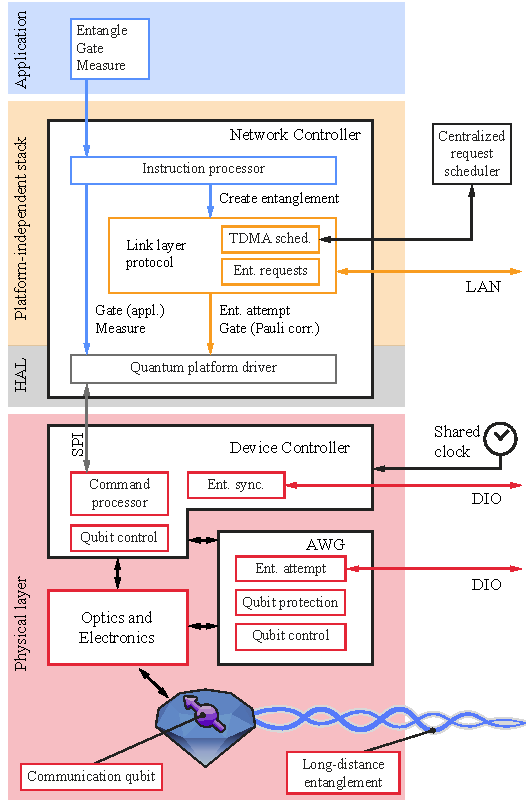
\includegraphics[width=0.6\linewidth]{figures/netnode.pdf}
    \caption{
        Quantum network node architecture. From top to bottom: At the application layer, a simple
        platform-independent routine is sent to the network controller. The network controller
        implements the platform-independent stack --- in this work only the link layer protocol ---
        and a \acrfull{hal} to interface with the physical layer's device controller. An instruction
        processor dispatches instructions either directly to the physical layer, or to the link
        layer protocol in case a remote entangled state is requested by the application. The link
        layer schedules entanglement requests and synchronizes with the remote node (on a local area
        network) using a \acrfull{tdma} schedule computed by a centralized scheduler (external). At
        the physical layer, the device controller fetches commands from --- and replies with
        outcomes to --- the network controller. Driven by a clock shared with the neighboring node,
        it performs hard-real-time synchronization for entanglement generation using a \acrfull{dio}
        interface. By controlling the optical and electronic components (among which an
        \acrlong{awg}, \acrshort{awg}), the device controller can perform universal quantum control
        of the communication qubit in real-time, as well as attempt long-distance entanglement
        generation with the neighboring node.
    }
    \label{fig:netnode}
\end{figure}

The original design of the \acrshort{qegp} and \acrshort{mhp} protocols, as well as our revision,
specifies the conceptual interaction between the two protocols and the service exposed to a higher
layer in the system, but does not impose particular constraints on how to implement link layer and
physical layer, how to realize the physical interface between them, and how to configure things such
as the centralized request scheduler and the entanglement attempt procedure. \Cref{fig:netnode}
gives an overview of the architecture of our quantum network nodes. We briefly describe our most
relevant implementation choices here and in the physical layer section.

\paragraph{Application processing}

At the application layer, user programs --- written in Python using a dedicated \emph{software
development kit}~\cite{netqasm_sdk} --- are processed by a rudimentary compilation stage, which
translates abstract quantum networking applications into gates and operations supported by our
specific quantum physical platform. Such gates and operations are expressed in a low-level
assembly-like language for quantum networking applications called
\emph{NetQASM}~\cite{dahlberg_2022_netqasm}. As part of our software stack, we also include an
\emph{instruction processor}, conceptually placed above the link layer, which is in charge of
dispatching entanglement requests to \acrshort{qegp} and other application instructions to the
physical layer directly.

\paragraph{Interface}

Ref.~\cite{dahlberg_2019_egp} did not provide a specification of the interface to be exposed by the
physical layer. We designed this interface such that the physical layer can accept \emph{commands}
from the higher layer, specifically:
%
\begin{inlinelist}
    \item qubit initialization (\texttt{INI}),
    \item qubit measurement (\texttt{MSR}),
    \item single-qubit gate (\texttt{SQG}),
    \item entanglement attempt (\texttt{ENT}, or \texttt{ENM} for \emph{M}- or \emph{R}-type
          requests),
    \item pre-measurement gates selection (\texttt{PMG}, to specify in which basis to measure the
          qubit for \emph{M}- or \emph{R}-type requests).
\end{inlinelist}
For each command, the physical layer reports back an \emph{outcome}, which indicates whether the
command was executed correctly, and can bear the result of a qubit measurement and the Bell state
produced after a successful entanglement attempt. Our software stack also comprises a
\emph{\acrlong{hal}} (\acrshort{hal}) that sits below \acrshort{qegp} and the instruction processor.
The \acrshort{hal} encodes and serializes commands and outcomes, and is thus used to interface with
the device controller.

\paragraph{TDMA network schedule}

Designing a full-blown centralized request scheduler is a challenge in and of its own, outside the
scope of this work. Instead of implementing such a scheduler, we compute static \acrshort{tdma}
network schedules~\cite{skrzypczyk_2021_arch} and install them manually on the two network nodes
upon initialization. \acrshort{tdma} network schedules are redundant in a one-link network.
Time-binning network activity also forces nodes to only process entanglement requests at the
beginning of a time division, thus introducing latency and idle time. Particularly, longer time bins
potentially result in entanglement requests to wait longer to be processed. However, an application
asking for multiple entangled pairs with just one request would experience smaller average
latencies, as all pairs—but the first one—would be generated in close succession.

\acrshort{tdma} schedules for our simple single-link experiments are quite trivial, as the network
resources of a node are not contended by multiple links. In particular, schedules are just a
constant division of \qty{20}{\ms} time bins, each of which is reserved to the only application
running. We chose the duration of the time-bin --- somewhat arbitrarily, given the small effect on
our experiments --- to be equal to \num{1000} communication cycles between the device controller and
the network controller ($\qty{20}{\ms} = \num{1000} × \qty{20}{\us}$).

\paragraph{Entanglement attempts}

Producing entanglement on a link can take several attempts. To minimize the number of \texttt{ENT}
commands fetched by \acrshort{mhp} from \acrshort{qegp}, as well as to mitigate the \acrshort{mhp}
synchronization overhead incurred after each entanglement command, we batch entanglement attempts at
the \acrshort{mhp} layer, such that synchronization and outcome reporting only happens once per
batch of attempts.

\paragraph{Delivered entangled states}

In our first iteration, we implemented \acrshort{qegp} such that it always delivers $\ket{\Phi^+}$
Bell states to the higher layer. This means that, when the physical layer produces a different Bell
state, \acrshort{qegp} (on the node where the entanglement request originates) issues a single-qubit
gate --- a Pauli correction --- to transform the entangled pair into the $\ket{\Phi^+}$ state (we
abbreviate the four two-qubit maximally entangled Bell states as $\ket{\Phi^\pm} = (\ket{00} \pm
\ket{11})/\sqrt{2}$ and $\ket{\Psi^\pm} = (\ket{01} \pm \ket{10})/\sqrt{2}$). A future version of
\acrshort{qegp} could allow the user to request any Bell state, and could extract the Pauli
correction from \acrshort{qegp} so that the application itself can decide, depending on the use
case, whether to apply the correction or not.

\paragraph{Mismatch verification}

As per our design specification, \acrshort{mhp} should also be responsible for verifying that the
entanglement commands coming from the two \acrshort{qegp} peers belong to the same request. We did
not implement this feature yet because, in our simple quantum network, we do not expect losses on
the classical channel used by the two \acrshort{mhp} parties to communicate --- a lossy classical
channel would be the primary source of inconsistencies at the \acrshort{mhp}
layer~\cite{dahlberg_2019_egp}. However, we believe that this verification step will prove very
useful in real-world networks where classical channels do not behave as predictably.

\paragraph{Deployment}

We implemented \acrshort{qegp} as a software module in a system that also includes the instruction
processor and the hardware abstraction layer. \acrshort{qegp}, the instruction processor and the
hardware abstraction layer, forming the \emph{network controller}, are implemented as a C/C++
standalone runtime developed on top of FreeRTOS, a real-time operating system for embedded
platforms~\cite{freertos}. The runtime and the underlying operating system are deployed on a
dedicated Avnet MicroZed --- an off-the-shelf platform based on the Zynq-7000 SoC, which hosts two
ARM Cortex-A9 processing cores, of which only one is used, clocked at \qty{667}{\MHz}.
\acrshort{qegp} connects to its remote peer via \acrshort{tcp} over a Gigabit Ethernet interface.
The interface to the physical layer is realized through a \qty{12.5}{\MHz} \acrshort{spi}
connection. The user application is sent from a general-purpose 4-core desktop machine running
Linux, which connects to the instruction processor through the same Gigabit Ethernet interface that
\acrshort{qegp} uses to communicate with its peer.

\section{Physical Layer Control in Real-Time}
\label{sec:netstack:phys}

In this section, we outline the design and operation of the physical layer, which executes the
commands issued by the higher layers on the quantum hardware and handles time-critical
synchronization between the quantum network nodes. The physical layer of a quantum network, as
opposed to the apparatus of a physics experiment, needs to be able to execute commands coming from
the layer above in real-time. Additionally, when performing the requested operations, it needs to
leave the quantum device in a state that is compatible with future commands (for example, as
discussed below, it should protect qubits from decoherence while it awaits further instructions).
Finally, if a request cannot be met (e.g.~the local quantum hardware is not ready, the remote
quantum hardware is not available, etc.), the physical layer should notify the link layer of the
issue without interrupting its service.

Our quantum network is composed of two independent nodes based on diamond \acrshort{nv} centers
physically separated by \qty{\approx 2}{m} (see \cref{fig:netnode} for the architecture of one
node). We will refer to the two nodes as \emph{client} and \emph{server}, noting that this is only a
logical separation useful to describe the case studies --- the two nodes have the exact same
capabilities. On each node, we implement the logic of the physical layer in a state-machine-based
algorithm deployed on a time-deterministic microcontroller, the \emph{device controller} (J\"ager
ADwin Pro II, based on Zynq-7000 SoC, dual-core ARM Cortex-A9, clocked at \qty{1}{\GHz}).
Additionally, each node uses an arbitrary waveform generator (\acrshort{awg}, Zurich Instruments
HDAWG8, \qty{2.4}{GSa/s}, \qty{300}{\MHz} sequencer) for nanosecond-resolution tasks, such as fast
optical and electrical pulses; the use of such a user-programmable \acrshort{fpga}-based
\acrshort{awg}, as opposed to a more traditional upload-and-play instrument (such as the ones used
in Ref.~\cite{pompili_2021_multinode}), enables the real-time control of our quantum device.

\paragraph{Single node operation}

On our quantum platform, before a node is available to execute commands, it needs to perform a qubit
readiness procedure called \emph{\acrlong{crcheck}} (\acrshort{crcheck}). This ensures that the
qubit system is in the correct charge state and that the necessary lasers are resonant with their
respective optical transitions. Other quantum platforms might have a similar preparation step, such
as loading and cooling for atoms and ions~\cite{stephenson_2020_highrate, ritter_2012_elementary}.
Once the \acrshort{crcheck} is successful, the device controller can fetch a command from the
network controller. Depending on the nature of the command, the device controller might need to
coordinate with other equipment in the node or synchronize with the device controller of the other
node.

For qubit initialization and measurement commands (\texttt{INI} and \texttt{MSR}), the device
controller shines the appropriate laser for a pre-defined duration
(\texttt{INI}\qty{\approx100}{\us}, \texttt{MSR}\qty{\approx10}{\us}). Both operations are
deterministic and carried out entirely by the device controller.

Single qubit gates (\texttt{SQG}) require the coordination of the device controller and the
\acrshort{awg}. For our communication qubits, they consist of generating an electrical pulse with
the \acrshort{awg} (duration \qty{\approx100}{\ns}), which is then multiplied to the qubit frequency
(\qty{\approx2}{\GHz}), amplified and finally delivered to the quantum device. The link layer can
request rotations in steps of $\pi/16$ around the X, Y or Z axis of the Bloch sphere (here we
implement only X and Y rotations, Z rotations will be implemented in the near future, see
\cref{app:phys}). When a new gate is requested by the link layer, the device controller at the
physical layer informs the \acrshort{awg} of the gate request via a parallel \num{32}-bit
\acrshort{dio} interface. The \acrshort{awg} will then select one of the $64$ pre-compiled
waveforms, play it, and notify the device controller that the gate has been executed. The device
controller will in turn notify the network controller of the successful operation.

After the rotation has been performed, our qubit --- if left idling --- would lose coherence in
\qty{\approx5}{\us}. A coherence time exceeding \qty{1}{s} has been reported on our
platform~\cite{abobeih_2018_one_sec} using decoupling sequences (periodic rotations of the qubit
that shield it from environmental noise). By interleaving decoupling sequences and gates, one can
perform extended quantum computations~\cite{bradley_2019_one_min}. These long sequences of pulses
have in the past been calculated and optimized offline (on a PC), then uploaded to an
\acrshort{awg}, and finally executed on the quantum devices with minimal interaction capabilities
(mostly binary branching trees, see~\cite{pompili_2021_multinode}). In our case, it is impossible to
pre-calculate these sequences, since we cannot know in advance which gates are going to be requested
by the link layer. To solve this challenge, we implement a {qubit protection} module on the
\acrshort{awg}, that interleaves decoupling sequences with the requested gates in real-time. As soon
as the first gate in a sequence is requested, the \acrshort{awg} starts a decoupling sequence on the
qubit. Then, it periodically checks if a new gate has been requested, and if so, it plays it at the
right time in the decoupling sequence. The \acrshort{awg} will continue the qubit protection routine
until the device controller will ask for it to stop (e.g.~to perform a measurement). This technique
allows us to execute universal qubit control without prior knowledge of the sequence to be played,
and --- crucially --- in real-time.

\paragraph{Entanglement generation}

Differently from the commands previously discussed, attempting entanglement generation
(\texttt{ENT}) requires tight timing synchronization between the device controllers --- and
\acrshortpl{awg} --- of the two nodes. In our implementation, the two device controllers share a
common \qty{1}{MHz} clock as well as a \acrshort{dio} connection to exchange synchronization
messages (see Ref.~\cite{pompili_2021_multinode}). When the device controllers are booted, they
synchronize an internal cycle counter that is used for time-keeping, and is shared, at each node,
with their respective network controllers to provide timing information to the link layer and the
higher layers. Over larger distances, one could use well-established protocols to achieve
sub-nanosecond, synchronized, \acrshort{gps}-disciplined common clocks~\cite{whiterabbit}.

When a device controller fetches an \texttt{ENT} command, it starts a three-way handshake procedure
with the device controller of the other node. If the other node has also fetched an \texttt{ENT}
command, they will synchronize and proceed with the entanglement generation procedure. If one of the
two nodes is not available (e.g.~it is still trying to pass the \acrshort{crcheck}) the other node
will time out, after \qty{0.5}{\ms}, and return an \emph{entanglement synchronization failure}
(\texttt{ENT\_SYNC\_FAIL}) to its link layer. The duration of the timeout is chosen such that is
comparable with the average time taken by a node to pass the \acrlong{crcheck} (if correctly on
resonance). This is to avoid unnecessary interactions between physical layer and link layer. After
the entanglement synchronization step, the device controllers proceed with an optical phase
stabilization cycle~\cite{pompili_2021_multinode}, and then the \acrshortpl{awg} are triggered to
attempt entanglement generation. In our implementation, one device controller (the server's)
triggers both \acrshortpl{awg} to achieve sub-nanosecond jitter between the two \acrshortpl{awg}
(see \cref{app:phys} for a discussion on longer distance implementation). Each entanglement attempt
lasts \qty{3.8}{\us}, and includes fast qubit initialization, communication-qubit to flying-qubit
entanglement, and probabilistic entanglement swapping of the flying
qubits~\cite{pompili_2021_multinode}. The \acrshortpl{awg} attempt entanglement up to \num{1000}
times before timing out and reporting an {entanglement failure} (\texttt{ENT\_FAIL}). Longer batches
of entanglement attempts would increase the probability that one of the nodes goes into the unwanted
charge state (and therefore cannot produce entanglement, see \cref{app:phys}). While in principle
possible, we did not implement, in this first realization, the charge stabilization mechanism
proposed in Ref.~\cite{humphreys_2018_delivery} that would allow for significantly longer batches of
entanglement attempts.

If an entanglement generation attempt is successful (probability \num{\approx 5e-5}), the
communication qubits of the two nodes will be projected into an entangled state (either
$\ket{\Psi^+}$ or $\ket{\Psi^-}$, depending on which detector clicked at the heralding station). To
herald success of the entanglement attempt, a \acrshort{cpld} (\acrlong{cpld}, Altera MAX V
5M570ZF256C5N) sends a fast digital signal to both \acrshortpl{awg} and device controllers, to
prevent a new entanglement attempt from being played (which would destroy the generated entangled
state). When the heralding signal is detected, the \acrshortpl{awg} enter the qubit protection
routine and wait for further instructions from the device controllers, which in turn notify the link
layer of the successful entanglement generation, as well as which state was generated.

To satisfy \emph{M}- or \emph{R}-type entanglement requests, the link layer can instruct the
physical layer to apply an immediate measurement to the entangled qubit by means of an \texttt{ENM}
command. Up until heralding of the entangled state, the physical layer operates as it does for the
\texttt{ENT} command. When the state is ready, it proceeds immediately with a sequence of single
qubit gates (as prescribed by an earlier \texttt{PMG} command) and a qubit measurement. The result
of the measurement, together with which entangled state was generated, is communicated to the link
layer. It is worth noting that the two nodes could fetch different types of requests and still
generate entanglement. In fact, this will be used later in the remote state preparation application.

\section{Evaluation}
\label{sec:netstack:eval}

To demonstrate and benchmark the capabilities of the link layer protocol, the physical layer, and of
our system as a whole, we execute --- on our two-node network --- three quantum networking
applications, all having a similar structure: the client asks for an entangled pair with the server,
which \acrshort{qegp} delivers in the $\ket{\Phi^+}$ Bell state, and then both client and server
measure their end of the pair in a certain basis. First, we perform full quantum state tomography of
the delivered entangled states. Second, we request and characterize entangled states of varying
fidelity. Third, we execute remote preparation of qubit states on the server by the client. For all
three applications, we study the quality of the entangled pairs delivered by our system.
Additionally, we use the second application to assess the latency incurred by our link layer, and to
compare it to the overall entanglement generation latency, including that of the physical layer.
Crucially, the three applications are executed back-to-back on the quantum network, without any
software or hardware changes to the system --- the only difference being the
quantum-platform-independent application sent to the instruction processor.

The sequence diagram in \cref{fig:fstomography}a exemplifies the general flow between system
components during the execution of an application. At first, the instruction processor issues a
request to create entanglement to link layer (\texttt{CREATE}). Then, the client's link layer
forwards the request with the server's counterpart (Forward \texttt{CREATE}). The request is
processed as soon as the designated time bin in the \acrshort{tdma} schedule starts, at which point
the first entanglement command (\texttt{ENT}) is fetched by physical layer. After an entangled state
is produced successfully (\texttt{PSI\_PLUS}), the link layer of the client issues, if needed, a
Pauli correction ($\pi$ rotation around the X axis, \texttt{SQG X180}) to deliver the pair in the
$\ket{\Phi^+}$ state. Finally, the instruction processor issues a gate ($\pi/2$ rotation around the
X axis, \texttt{SQG X90}) and a measurement (\texttt{MSR}) to read out the entangled qubit in a
certain basis, and receives an outcome from the physical layer (\texttt{0}).
\Cref{fig:fstomography}b illustrates the actual latencies between these interactions in one
iteration of the full state tomography application.

\begin{figure}[t]
    \centering
    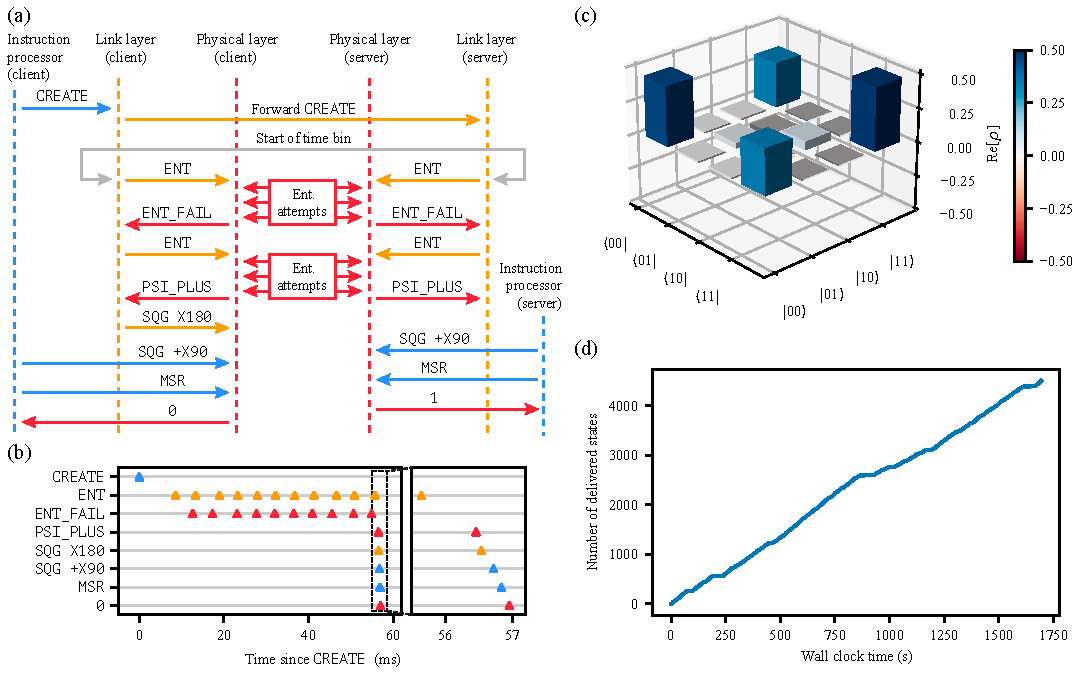
\includegraphics[width=\linewidth]{figures/fstomography.pdf}
    \caption{
        Full state tomography with the quantum network stack.
        %
        (a) Sequence diagram of the communication steps across the network stack and the two nodes
        to perform one repetition of the tomography application (in particular, measurement of the
        $\braket{YY}$ correlator). The coloring follows that of \cref{fig:netstack}.
        \texttt{CREATE}: entanglement request, \texttt{ENT}: entanglement attempts request,
        \texttt{ENT\_FAIL}: failed the batch of entanglement attempts, \texttt{PSI\_PLUS}:
        successful entanglement attempt with generated state $\Psi^+$, \texttt{SQG}: single-qubit
        gate, \texttt{X180}: \ang{180} rotation around X axis, \texttt{MSR}: qubit measurement,
        \texttt{0/1}: qubit measurement outcome. Note that the client's link layer protocol requests
        a \texttt{X180} gate after entanglement generation to deliver the $\ket{\Phi^+}$ Bell state
        to the higher layer.
        %
        (b) Example time trace of (a) for the client. Several batches of entanglement attempts are
        required before an entangled state is heralded. On the right, a zoomed-in part of the trace
        (corresponding to the dashed box in the left plot).
        %
        (c) Reconstructed density matrix of the states delivered by the link layer. Only the real
        part is plotted (imaginary elements are all \num{\approx 0}, see main text). We estimate a
        fidelity F with $\ket{\Phi^+}$ of $F =$ \num{0.783(7)}.
        %
        (d) Total number of delivered states over time. The occasional pauses in entanglement
        delivery (plateaus) are due to the client's \acrshort{nv} center becoming off-resonant with
        the relevant lasers (see \cref{app:phys}). Differences in slope are due to changes in
        resonance conditions that increase the time necessary to pass the \acrlong{crcheck}.
    }
    \label{fig:fstomography}
\end{figure}

For all our experiments, we configured \acrshort{tdma} time bins to be of \qty{20}{\ms}. In a larger
network, the duration of time bins should be calibrated according to the average time it takes, on a
certain link, to produce an entangled pair of a certain fidelity~\cite{skrzypczyk_2021_arch}. By
doing so, one can maximize network usage and thus reduce qubit decoherence on longer end-to-end
paths. However, in our single-link network, the duration of time bins only influences the frequency
at which new entanglement requests are processed. Our time bin duration accommodates up to four
batches of \num{1000} entanglement attempts.

\note{Perhaps we could open-source the NetQASM application scripts for this evaluation and add a
link to the repository here.}

\paragraph{Full quantum state tomography}

The first application consists in generating entangled states at the highest \emph{minimum fidelity}
currently available on our physical setup (\num{0.80}), and measuring the two entangled qubits in
varying bases to learn their joint quantum state. We measure all \num{9} two-node correlators
($\braket{\mathrm{XX}}, \braket{\mathrm{XY}}$, ...,~$\braket{\mathrm{ZZ}}$) as well as all their
$\pm$ variations ($\braket{\mathrm{+X+X}}, \braket{\mathrm{+X-X}}$, etc.) to minimize the bias due
to measurement errors. For each of the $9 \times 4 = 36$ combinations, we measure \num{125} data
points, for a total of \num{4500} entangled states generated and measured.

The collected measurement outcomes are then analyzed using QInfer~\cite{granade_2017_qinfer}, in
particular the Monte Carlo method described in Ref.~\cite{granade_2016_practical} for Bayesian
estimation of density matrices from tomographic measurements. The reconstructed density matrix is
displayed in \cref{fig:fstomography}c (only the real part is shown) and its values and uncertainties
are
%
\begin{equation*}
    \mathrm{Re}[\rho] = \begin{pmatrix}
        0.442(6) & 0.003(3)  & 0.003(2)  & 0.328(5)  \\
        0.003(3) & 0.033(6)  & -0.023(5) & -0.000(5) \\
        0.003(2) & -0.023(5) & 0.056(4)  & -0.003(4) \\
        0.328(5) & -0.000(5) & -0.003(4) & 0.469(7)  \\
    \end{pmatrix},
\end{equation*}
%
\begin{equation*}
    \mathrm{Im}[\rho] = \begin{pmatrix}
        0         & -0.014(3) & -0.005(7) & 0.032(5)  \\
        0.014(3)  & 0         & -0.002(4) & 0.001(5)  \\
        0.005(7)  & 0.002(4)  & 0         & -0.000(7) \\
        -0.032(5) & -0.001(5) & 0.000(7)  & 0         \\
    \end{pmatrix}.
\end{equation*}
Here $\rho_{ij, mn} = \braket{ij|\ \rho\ |mn}$, with $i,m$ ($j,n$) being the client (server) qubit
states in the computational basis. The uncertainty on each element of the density matrix is
calculated as the standard deviation of that element over the probability distribution approximated
by the Monte Carlo reconstruction algorithm (probability distribution approximated by \num{1E5}
Monte Carlo particles~\cite{granade_2016_practical}). It is then possible to estimate the fidelity
of the delivered entangled states with respect to the maximally entangled Bell state, which we find
to be $F =$ \num{0.783(7)}. The measured fidelity is slightly lower (\qty{\approx 3}{\percent}) than
what measured in Ref.~\cite{pompili_2021_multinode} without the use of the \acrshort{qegp}
abstraction (and the whole network controller where \acrshort{qegp} runs). This discrepancy could be
due to the additional physical-layer decoupling sequences required for real-time operation
(\qty{\approx 300}{\us}) and the additional single-qubit gate issued by the link layer to always
deliver $\ket{\Phi^+}$ (the physical layer can produce either $\ket{\Psi^+} = (\ket{01} +
    \ket{10})/\sqrt{2}$ or $\ket{\Psi^-} = (\ket{01} - \ket{1})/ \sqrt{2}$, see
Refs.~\cite{humphreys_2018_delivery, pompili_2021_multinode}).

It is to be noted that, in order to obtain the most faithful estimate of the generated state
(see \cref{sec:netstack:corrections} for details), the measured expectation values are corrected, in
post-processing, to remove known tomography errors of both client and
server~\cite{nachman_2020_unfolding}, and events in which at least one physical device was in the
incorrect charge state.

Finally, we show, in \cref{fig:fstomography}d, that our system can sustain a fairly stable
entanglement delivery rate over \qty{\approx 30}{min} of data acquisition --- plateaus and changes
in slope can be attributed to varying conditions of resonance between the \acrshort{nv} centers and
the relevant lasers (see \cref{app:phys}).

\paragraph{Latency VS fidelity}

The \acrshort{qegp} interface allows its user to request entangled pairs at various minimum
fidelities. For physical reasons, higher fidelities will result in lower entanglement generation
rates~\cite{stockill_2017_phasetuned, humphreys_2018_delivery}. The trade-off between fidelity and
throughput is particularly interesting in a scenario where some applications might require
high-fidelity entangled pairs and are willing to wait a longer time, while others might prefer
lower-fidelity states but higher rates~\cite{dahlberg_2019_egp}. Clearly, for the link layer to
offer a range of fidelities to choose from, the underlying physical layer must support such a range.
We benchmark the capabilities of the link layer and of the physical layer to deliver states at
various fidelities in a single application by measuring the $\braket{\mathrm{XX}}$,
$\braket{\mathrm{YY}}$ and $\braket{\mathrm{ZZ}}$ correlators (and their $\pm$ variations, as we did
above, for a total of $3 \times 4 = 12$ correlators) for seven different target fidelities,
(\num{0.50}, \num{0.55}, \num{0.60}, \num{0.65}, \num{0.70}, \num{0.75}, \num{0.80}). We generate
\num{1500} entangled states per fidelity, for a total of \num{10500} delivered states. With this
case study, we analyze both the resulting fidelity and the system's latency for different requested
fidelities.

\begin{figure}[t]
    \centering
    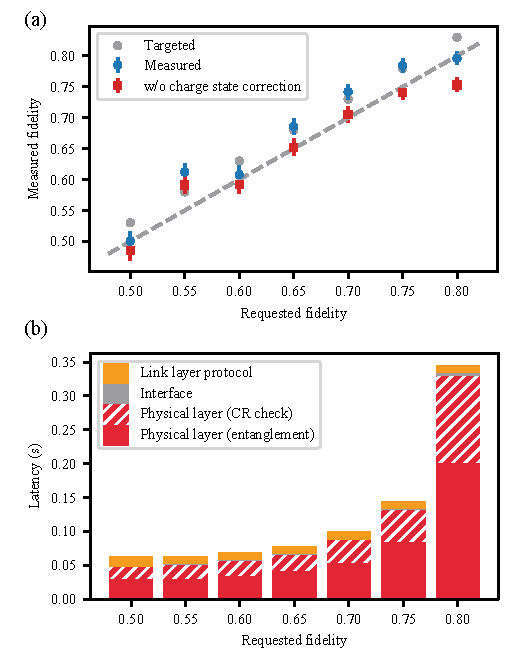
\includegraphics[width=0.6\linewidth]{figures/latencyvsfid.pdf}
    \caption{
        Performance of the entanglement delivery service.
        %
        (a) Measured fidelity of the states delivered by the link layer for varying requested
        fidelity. Targeted fidelity at the physical layer is 0.03 higher than the link layer
        protocol's \emph{minimum fidelity} request. When not correcting for wrong charge state
        events, fidelity is reduced by a few percents (see \cref{sec:netstack:corrections}). Error
        bars represent \num{1} s.d.
        %
        (b) Average latency of the entanglement delivery per requested fidelity, broken down into
        sources of latency. Entanglement generation and \acrlong{crcheck} at the physical layer are
        the largest sources of latency (at higher fidelities, more entanglement attempts are
        required before success). Running the link layer protocol introduces a small but measurable
        overhead (\qty{\approx 10}{ms}) to the entanglement generation procedure, which does not
        depend on the requested fidelity, and that could be mitigated by requesting multiple
        entangled states in a single instruction. The communication delays between quantum network
        controller and quantum device controller (Interface) introduce negligible overall latency.
    }
    \label{fig:latencyvsfid}
\end{figure}

The results for measured fidelity versus requested fidelity are shown in \cref{fig:latencyvsfid}a.
It is worth noting that the application iterates over the range of fidelities in real-time, and thus
the physical layer is prepared to deliver any of them at any point. We calibrate the physical layer
to deliver states of slightly higher fidelity than the requested ones (\num{0.03} more), since
entanglement requests specify the \emph{minimum} desired fidelity. The measured fidelities are ---
within measurement uncertainty --- always matching or exceeding the requested minimum ones (the
dashed gray line in \cref{fig:latencyvsfid}a is the $y=x$ diagonal). As in the previous application,
measurement outcomes are post-processed to eliminate tomography errors and events in which the
physical devices were in the incorrect charge state (we refer to the latter as \emph{charge state
correction}). For arbitrary applications that use the delivered entangled states for something other
than statistical measurements, applying the second correction directly at the link layer might prove
challenging, since the information concerning whether to discard an entangled pair is only available
at the physical layer \emph{after} the entangled state is delivered to the link layer (when the next
\acrshort{crcheck} is performed). However, a mechanism to identify \emph{bad} entangled pairs
retroactively at the link layer --- like the expiry functionality included in the original design of
\acrshort{qegp}~\cite{dahlberg_2019_egp} --- could be used to discard entangled states after they
have been delivered by the physical layer. For completeness, we also report, again in
\cref{fig:latencyvsfid}a, the measured fidelity when the wrong charge state correction is not
applied.

For each requested fidelity we also measure the entanglement generation
latency~\cite{dahlberg_2019_egp}, defined as the time between the issuing of the \texttt{CREATE}
request to the link layer, until the successful entanglement outcome reported by the physical layer
(refer to \cref{fig:fstomography}a for a diagram of the events in between these two).
\Cref{fig:latencyvsfid}b shows the measured average latency, grouped by requested fidelity and
broken down into the various sources of latency. When calculating the average latencies, we have
ignored entanglement requests that required more than \qty{10}{s} to be fulfilled. These
high-latency requests correspond to the horizontal plateaus of \cref{fig:fstomography}d. The main
contribution to the total latency comes from the entanglement generation process at the physical
layer, followed by the \acrshort{nv} center preparation time (\acrshort{crcheck}). Both latency
values are consistent with the expected number of entanglement attempts required by the
single-photon entanglement protocol employed at the physical layer~\cite{humphreys_2018_delivery}.
The link layer protocol adds, on average, \qty{\approx 10}{\ms} of extra latency to all requests,
regardless of their fidelity. This is due partly to the synchronization of the \texttt{CREATE}
request between the two nodes (i.e.~a simple \acrshort{tcp} message), but mostly to the nodes having
to wait for the next time bin in the network schedule to start. We remark that, by requesting
multiple entangled states in a single \texttt{CREATE}, one can distribute this overhead over many
generated pairs, to the point where it becomes negligible. While our applications did not issue
multi-pair \texttt{CREATE} requests, this would be the more natural choice for real applications,
and would result in better utilization of the allocated time bins. Finally, the overhead incurred by
the interface between microcontrollers is rather small (barely visible in \cref{fig:latencyvsfid}b),
but could however be further reduced by integrating device controller and network controller into a
single device. It is worth mentioning that, in our simple scenario in which each entanglement
request is only submitted to \acrshort{qegp} after the previous one completes, and thus the request
queue never grows larger than one element, throughput happens to be almost exactly the same as the
inverse of latency, and hence it is not reported here.

Overall, we observe that the extra entanglement generation latency incurred when deploying an
abstraction layer (\acrshort{qegp}) on top of the physical layer, while not too modest, is only a
small part of the whole, particularly at higher fidelities. Nevertheless, optimizing the length of
\acrshort{tdma} time bins could result in an even smaller overhead.

\begin{figure}[t]
    \centering
    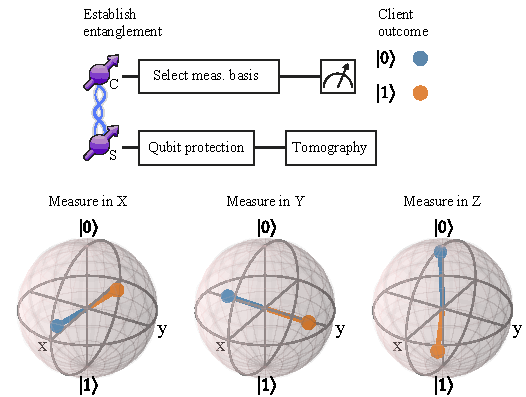
\includegraphics[width=0.6\linewidth]{figures/rsprep.pdf}
    \caption{
        Tomography of states prepared on the server by the remote client. For each chosen
        measurement axis of the client (X, Y, Z), and for each obtained measurement outcome at the
        client ($\ket{0}$, $\ket{1}$), a different state is prepared on the server. Plotted on the
        Bloch spheres are the results of the tomography on the server's qubit. Uncertainties on each
        coordinate are \num{\approx 0.05} (see \cref{sec:netstack:corrections}). We find an average
        fidelity of $F =$ \num{0.853(8)}.
    }
    \label{fig:rsprep}
\end{figure}

\paragraph{Remote state preparation}

One of the use cases of the \acrshort{qegp} service is to prepare quantum states on a remote
server~\cite{dahlberg_2019_egp}. Remote state preparation is a fundamental step to execute a blind
quantum computation application~\cite{broadbent_2009_ubqc}, whereby a client quantum computer with
limited resources can run applications on a powerful remote quantum server using the many qubits the
server has, while keeping the performed computation private.

Remote state preparation is different from the previous two cases in that the client can measure its
end of the entangled pair as soon as the pair is generated, while the server has to keep its qubit
alive waiting for further instructions. For such a scenario, the client can make use of
\acrshort{qegp}'s service to issue \emph{R}-type entanglement requests, so that the local end of the
entangled pair can be measured (in a certain basis) as soon as it is generated, while the server's
qubit can be protected for later usage. An \emph{R}-type entanglement request results in an
\texttt{ENM} command on the client and an \texttt{ENT} command on the server. For this type of
requests (as well as for \emph{M}-type ones), since the local end of the pair is measured
immediately, the client's \acrshort{qegp} can skip the Pauli correction used to always deliver
$\ket{\Phi^+}$, and can instead apply a classical correction to the received measurement outcome.

To showcase this feature of \acrshort{qegp} we use the client node to prepare the six cardinal
states on the server ($\ket{\pm x}$, $\ket{\pm y}$, $\ket{0}$ and $\ket{1}$) by having the client
measure its share of the entangled state in the six cardinal bases. We then let the server measure
the prepared states --- again in the six cardinal bases --- to perform tomography. For each client
measurement basis, and for each server tomography basis, we deliver \num{125} entangled states at a
requested fidelity of \num{0.80}, for a total of $6 \times 6 \times 125 = 4500$ remote state
preparations. The results are presented in \cref{fig:rsprep}, which displays the tomography of the
prepared states on the server, for the three different measurement axes of the client and the two
possible measurement outcomes of the client. The prepared states are affected by the measurement
error of the client ($F_0 =$ \num{0.928(3)}, $F_1 = $ \num{0.997(1)}): an error in the measurement
of the client's qubit results in an incorrect identification of the state prepared on the server. By
alternating between positive and negative readout orientations, we make sure that the errors affect
all prepared states equally, instead of biasing the result. We note that we exclude, once again,
events in which at least one of the two devices was in the wrong charge state, and we correct for
the known tomography error on the server (results without corrections are in
\cref{sec:netstack:corrections}). Overall, we find an average remote state preparation fidelity of
$F =$ \num{0.853(8)}. The asymmetry in the fidelity of the $\ket{0}$ and $\ket{1}$ states is caused
by the asymmetry in the populations $\braket{01|\ \rho\ |01}$ vs $\braket{10|\ \rho\ |10}$ of the
delivered entangled state, which in turn is due to the double $\ket{0}$ occupancy error of the
single-photon protocol used to generate entanglement~\cite{humphreys_2018_delivery,
pompili_2021_multinode}.

\section{Results With and Without Corrections}
\label{sec:netstack:corrections}

The data presented in the main text is corrected for known measurement errors, and events in which
at least one of the two devices was in the wrong charge state are removed (the \acrshort{crcheck}
following the delivery of entanglement reports zero counts). While it is useful to correct for such
errors in order to obtain the most faithful reconstruction of the delivered states, these errors
cannot always be avoided in a real network scenario. For completeness, we report here the results
first without any corrections applied, and then with only the measurement error correction applied.
All the results, the raw datasets, and the software to analyze them, are available at
Ref.~\cite{link_layer_data}.

\paragraph{Full quantum state tomography}

The events in which the two devices generated \num{0} photon counts in the following
\acrshort{crcheck} were \num{37} for the client and \num{380} for the server (out of the \num{4500}
total). When combined, (client or server in the wrong charge state), we obtain \num{417} events (in
zero events both client and server were in the wrong charge state). Without any corrections
(tomography errors or wrong charge state), we obtain the following density matrix (which has a
fidelity with the target Bell state F=\num{0.681(16)}):
\[
    \mathrm{Re}[\rho] = \begin{pmatrix}
        0.397(9)  & 0.011(9)   & 0.001(7)   & 0.256(14)  \\
        0.011(9)  & 0.058(14)  & -0.005(13) & -0.007(9)  \\
        0.001(7)  & -0.005(13) & 0.092(12)  & -0.027(13) \\
        0.256(14) & -0.007(9)  & -0.027(13) & 0.452(9)   \\
    \end{pmatrix},
\]
\[
    \mathrm{Im}[\rho] = \begin{pmatrix}
        0          & 0.000(18)  & -0.029(9) & 0.036(9)  \\
        -0.000(18) & 0          & 0.010(12) & -0.002(8) \\
        0.029(9)   & -0.010(12) & 0         & -0.000(8) \\
        -0.036(9)  & 0.002(8)   & 0.000(8)  & 0         \\
    \end{pmatrix}
\]

Only applying tomography error correction (but not removal of wrong charge state events) yields the
following density matrix (fidelity F=\num{0.744(11)}):
\[
    \mathrm{Re}[\rho] = \begin{pmatrix}
        0.421(7)  & -0.001(4) & -0.013(5) & 0.300(8)  \\
        -0.001(4) & 0.022(8)  & -0.020(6) & -0.021(7) \\
        -0.013(5) & -0.020(6) & 0.091(5)  & -0.015(5) \\
        0.300(8)  & -0.021(7) & -0.015(5) & 0.466(5)  \\
    \end{pmatrix}
\]
\[
    \mathrm{Im}[\rho] = \begin{pmatrix}
        0         & 0.004(4)  & -0.018(3) & 0.032(6) \\
        -0.004(4) & 0         & 0.021(6)  & 0.002(5) \\
        0.018(3)  & -0.021(6) & 0         & 0.002(5) \\
        -0.032(6) & -0.002(5) & -0.002(5) & 0        \\
    \end{pmatrix}
\]


\paragraph{Fidelity VS rate}

The events in which the two devices generated \num{0} photon counts in the following
\acrshort{crcheck} were \num{74} for the client and \num{709} for the server (out of the \num{10500}
total). When combined, (client or server in the wrong charge state), we obtain \num{781} events
(there were two events in which both client and server were in the wrong charge state). Without any
corrections (tomography errors or wrong charge state), we obtain the following delivered fidelities:
\num{0.454(18)}, \num{0.540(18)}, \num{0.548(17)}, \num{0.596(17)}, \num{0.640(16)},
\num{0.674(16)}, \num{0.679(15)}. Only applying tomography error correction (but not removal of
wrong charge state events) yields the following fidelities: \num{0.485(15)}, \num{0.591(14)},
\num{0.592(14)}, \num{0. 652(13)}, \num{0.705(13)}, \num{0.741(12)}, \num{0.753(11)}.

\paragraph{Remote state preparation}

As mentioned in the main text, for the remote state preparation analysis, we only apply the
tomography error correction for the server, while remove wrong charge state events of both the
server and the client. The events in which the two devices generated \num{0} photon counts in the
following \acrshort{crcheck} were \num{29} for the client and \num{365} for the server (out of the
\num{4500} total). When combined, (client or server in the wrong charge state), we obtain \num{394}
events (there were zero events in which both client and server were in the wrong charge state).
Following are the numerical values that result in the plot in the main text (average fidelity
F=\num{0.853(8)}):

\begin{table}[H]
    \centering
    % with_m_error_correction_with_ionization_correction
    \begin{tabular}{|p{2.5cm}|ccc|c|}
        \hline
        Client & \multicolumn{4}{c|}{Server}\\
        & $\braket{\mathrm{X}}$ & $\braket{\mathrm{Y}}$ & $\braket{\mathrm{Z}}$ & Fidelity\\ \hline
        Measured $\ket{+X}$ & \num{0.634(48)} & \num{-0.123(62)} & \num{-0.004(59)} & \num{0.817(24)}\\
        Measured $\ket{+Y}$ & \num{-0.028(58)} & \num{-0.650(45)} & \num{0.005(61)} & \num{0.825(23)}\\
        Measured $\ket{+Z}$ & \num{-0.081(65)} & \num{-0.083(66)} & \num{0.849(31)} & \num{0.924(16)}\\
        Measured $\ket{-X}$ & \num{-0.645(43)} & \num{0.135(59)} & \num{0.030(63)} & \num{0.823(22)}\\
        Measured $\ket{-Y}$ & \num{0.026(65)} & \num{0.719(40)} & \num{-0.013(61)} & \num{0.860(20)}\\
        Measured $\ket{-Z}$ & \num{0.032(58)} & \num{-0.069(58)} & \num{-0.736(39)} & \num{0.868(19)}\\
        \hline
    \end{tabular}
    %==========
    %Avg F 0.853(8)
\end{table}

Without any corrections (tomography errors or wrong charge state), we obtain the following prepared
states, with average fidelity F=\num{0.807(10)}:

\begin{table}[H]
    \centering
    % without_m_error_correction_without_ionization_correction
    \begin{tabular}{|p{2.5cm}|ccc|c|}
        \hline
        Client & \multicolumn{4}{c|}{Server}\\
        & $\braket{\mathrm{X}}$ & $\braket{\mathrm{Y}}$ & $\braket{\mathrm{Z}}$ & Fidelity\\ \hline
        Measured $\ket{x}$ & \num{0.534(55)} & \num{-0.090(62)} & \num{0.009(62)} & \num{0.767(27)}\\
        Measured $\ket{y}$ & \num{0.024(60)} & \num{-0.582(51)} & \num{-0.013(62)} & \num{0.791(26)}\\
        Measured $\ket{0}$ & \num{-0.073(69)} & \num{-0.072(69)} & \num{0.786(42)} & \num{0.893(21)}\\
        Measured $\ket{-x}$ & \num{-0.552(49)} & \num{0.143(61)} & \num{0.055(63)} & \num{0.776(24)}\\
        Measured $\ket{-y}$ & \num{0.052(64)} & \num{0.623(47)} & \num{-0.018(62)} & \num{0.811(23)}\\
        Measured $\ket{1}$ & \num{0.030(57)} & \num{-0.028(55)} & \num{-0.606(46)} & \num{0.803(23)}\\
        \hline
    \end{tabular}
    %==========
    %Avg F 0.807(10)
\end{table}

When only applying tomography error correction, we find an average preparation fidelity F=\num{0.829(9)}:

\begin{table}[H]
    \centering
    % with_m_error_correction_without_ionization_correction
    \begin{tabular}{|p{2.5cm}|ccc|c|}
        \hline
        Client & \multicolumn{4}{c|}{Server}\\
        & $\braket{\mathrm{X}}$ & $\braket{\mathrm{Y}}$ & $\braket{\mathrm{Z}}$ & Fidelity\\ \hline
        Measured $\ket{x}$ & \num{0.573(49)} & \num{-0.096(59)} & \num{0.010(58)} & \num{0.786(24)}\\
        Measured $\ket{y}$ & \num{0.025(56)} & \num{-0.624(45)} & \num{-0.014(59)} & \num{0.812(23)}\\
        Measured $\ket{0}$ & \num{-0.078(64)} & \num{-0.077(65)} & \num{0.843(32)} & \num{0.921(16)}\\
        Measured $\ket{-x}$ & \num{-0.592(44)} & \num{0.153(57)} & \num{0.059(59)} & \num{0.796(22)}\\
        Measured $\ket{-y}$ & \num{0.056(61)} & \num{0.667(41)} & \num{-0.020(59)} & \num{0.834(20)}\\
        Measured $\ket{1}$ & \num{0.032(54)} & \num{-0.030(53)} & \num{-0.650(40)} & \num{0.825(20)}\\
        \hline
    \end{tabular}
    %==========
    %Avg F 0.829(9)
\end{table}

\section{Discussion}

In summary, we have demonstrated the operation of a link layer and a physical layer for
entanglement-based quantum networks. The link layer abstracts the entanglement generation procedure
provided by the physical layer --- implemented here with two \acrshort{nv} center-based quantum
network nodes --- into a robust platform-independent service that can be used to run quantum
networking applications. We performed full quantum state tomography of the states delivered by the
link layer, tested its ability to deliver states at different fidelities in real-time, and verified
remote state preparation of a qubit from the client on the server, a fundamental step towards blind
quantum computation~\cite{broadbent_2009_ubqc}. We have shown that our implementation of link and
physical layers can deliver entangled states at the fidelity requested by the user, despite some
marginal inefficiencies --- some of which can be addressed in a future version of the protocols
(e.g.~avoiding Pauli corrections unless necessary). We have also quantified the additional latency
incurred by deploying the link layer protocol on top of the physical layer. Although not
detrimental, the extra overhead is still noticeable, but can also be scaled down by optimizing the
scheduling of entanglement generation requests. We also acknowledge that scheduling a quantum node's
resources is still an open problem~\cite{skrzypczyk_2021_arch, vardoyan_2019_performance,
vardoyan_2021_capacity} and that the simple approach taken here is likely a suboptimal choice for
more advanced quantum networks. We emphasize, however, that our link layer protocol is not tied to
any particular scheduling algorithm or architecture --- it merely expects that the schedule of each
node be matched with its peer. In Ref.~\cite{dahlberg_2019_egp} for example, the schedule was
instead formed via a distributed queue protocol, and in the future other architectures and
algorithms~\cite{skrzypczyk_2021_arch} may be more suitable for scaling to larger networks.

Other research challenges posed by our work include an in-depth analysis of the security of quantum
network implementations. For example, it is clear that if the classical control messages used in our
protocol are not authenticated, unwanted entanglement generation may be triggered at one of the
nodes. In some physical layer implementations such as the one considered here, this may negatively
impact the quality of the qubits already stored at the node~\cite{kalb_2018_dephasing}, and hence
impact availability. Initial work indicates that the performance impact of adding authentication,
however, is small (refer to \cref{chp:doa}).

The adoption of the techniques presented here (which are not specific to our diamond devices) by
other quantum network platforms~\cite{ritter_2012_elementary, stockill_2017_phasetuned,
rose_2018_observation, nguyen_2019_quantum, stephenson_2020_highrate, trusheim_2020_transform,
son_2020_developing} will boost the development towards large-scale and heterogeneous quantum
networks. Real-time control of memory qubits, as well as the availability of multi-node networks and
dynamic network schedules, will enable demonstrations of the higher layers of the network
stack~\cite{kozlowski_2019_towards}, which in turn will open the door to end-to-end connectivity on
a platform-independent quantum network.

\printbibliography[heading=subbibintoc,title={References},notcategory=noprint]

\chapter{Quantum Networking With an Elementary Operating System}
\label{chp:qnodeos}

\begin{abstract}
An \acrfull{os} for quantum network nodes should provide more than just networking functionalities.
Ultimately, it should enable quantum networking applications to be written in high-level,
platform-independent software, and should be able to manage the resources of the underlying
device when deployed in a multi-node and multi-user quantum network. This chapter discusses our
implementation of \acrshort{qnodeos}, an \acrshort{os} for quantum network nodes, which includes a
quantum network stack for entanglement generation, as well as resource management and scheduling
features that allow the concurrent execution of multiple applications. We also design and propose a
set of benchmarks which will be used to quantify --- in upcoming work --- the performance of the
\acrshort{os} on state-of-the-art quantum network hardware based on \acrlong{nv} centers in diamond.
\end{abstract}

\blfootnote{
This chapter is extracted from the article in preparation:
\fullcite{delledonne_2023_qnodeos_noprint}.

Contributions: as indicated in \cref{chp:background}.
}

\newpage

\lettrine{T}{he} preliminary experiments conducted in \cref{chp:netstack} showcased elementary
quantum networking functionalities through a platform-independent control system --- mainly, the
quantum networking stack embedded in \acrshort{qnodeos}. Nevertheless, entanglement generation is
just one of the blocks constituting fully-fledged quantum communications applications, which also
include local quantum processing and classical communication and processing, as shown in
\cref{fig:app-struct}. With \acrshort{qnodeos}, we aim to take the state of the art of quantum
networking experiments one step further, and demonstrate the execution of complete applications,
some of which comprise quantum and classical processing and communication. We also include one case
study that serves as a proof-of-concept demonstration of the usefulness of a multitasking-ready
\acrshort{os}, to be expanded on when investigating multi-user quantum networks more in depth. In
this chapter we describe the proposed test applications, which will serve as case studies for the
upcoming evaluation of \acrshort{qnodeos} on \acrshort{nv} center devices. Prior to that, we also
give an overview of the implementation of \acrshort{qnodeos} and the underlying \acrshort{qdevice}.
Refer to \cref{app:qnodeos} for additional details on the implementation of the components of
\acrshort{qnodeos} and their interfaces, and to \cref{app:qdevice} for the specification of the
interface to the \acrshort{qdevice}.

\section{Implementation}
\label{sec:qnodeos:implementation}

\begin{figure}[b]
    \centering
    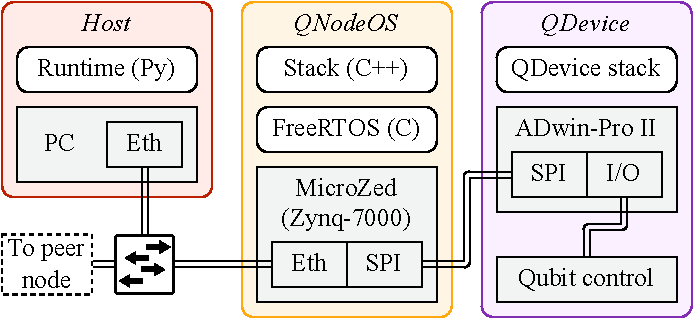
\includegraphics[width=0.6\linewidth]{figures/node-deployment.pdf}
    \caption{
        Node deployment overview. Our quantum network node consists of a desktop machine for the
        host runtime, a Zynq-7000 SoC for \acrshort{qnodeos}, and a series of digital and analog
        controllers for the \acrshort{qdevice}.
    }
    \label{fig:node-deployment}
\end{figure}

\Cref{fig:node-deployment} outlines software and hardware implementation of \acrshort{qnodeos} and
the whole node system. \acrshort{qnodeos} is implemented in C++ on top of FreeRTOS~\cite{freertos},
a tiny operating system for microcontrollers. The stack runs on a dedicated MicroZed~\cite{microzed}
--- an off-the-shelf platform based on the Zynq-7000 SoC, which hosts two ARM Cortex-A9 processing
cores, of which only one is used, clocked at \qty{667}{\MHz}. \acrshort{qnodeos} connects to peer
\acrshort{qnodeos} systems via \acrshort{tcp} over a Gigabit Ethernet interface. We opted for a
device like the Zynq-7000 SoC for its advantageous trade-off between high flexibility and moderate
cost (around €~100 in the Netherlands at the time of writing). Whilst more concrete device
requirements may arise from our future benchmarking of \acrshort{qnodeos}, we believe that the
selected SoC provides enough computational bandwidth for the envisioned tasks, and it also offers
the possibility to implement optimized hardware modules on its \acrshort{fpga} fabric. We however
remark that the design of \acrshort{qnodeos} is in no way tied to a certain computing architecture.
For the \acrshort{qdevice}, we replicated the setup used for \cref{chp:netstack}, which mainly
consists of:
%
\begin{inlinelist}
    \item an ADwin-Pro II~\cite{adwin} acting as the main orchestrator of the setup;
    \item a series of subordinate devices responsible for qubit control, including laser pulse
          generators and optical readout circuits;
    \item the quantum physical device, based on \acrshort{nv} centers, counting one single
          (communication) qubit for each node.
\end{inlinelist}
The \acrshort{qdevice} is where the time-critical qubit control lies. \acrshort{qnodeos} interfaces
with the \acrshort{qdevice}'s ADwin-Pro II through a \qty{12.5}{\MHz} \acrshort{spi} interface, used
to exchange 4-byte control messages at a rate of \qty{50}{kHz}. Finally, the host layer is a Python
runtime running on a general-purpose 4-core desktop machine running Linux. The host machine connects
to \acrshort{qnodeos} via \acrshort{tcp} over the same Gigabit Ethernet interface that
\acrshort{qnodeos} uses to connect to its peers (average ping \acrshort{rtt} of \qty{0.1}{\ms}), and
sends application registration requests and quantum code blocks over this interface (\num{10} to
\num{1000} bytes, depending on the length of the block).

\begin{table}[t]
    \centering
    \begin{tabularx}{\linewidth}{llrYYYY}
        \toprule
                                   &                    &                & \multicolumn{4}{c}{\textbf{Lines of code}}                           \\
        \cmidrule(l){4-7}
        \textbf{Component}         & \textbf{File type} & \textbf{Files} & \textbf{Total} & \textbf{Blanks} & \textbf{Comments} & \textbf{Code} \\
        \midrule
        \multirow{4}{*}{Core code} & C/C++              & 85             & 16273          & 2779            & 1953              & 11541         \\
                                   & C/C++ header       & 121            & 13281          & 2418            & 4188              & 6675          \\
                                   & CMake              & 25             & 486            & 99              & 43                & 344           \\
                                   & Assembly           & 1              & 141            & 15              & 0                 & 126           \\
        \midrule
        \multirow{4}{*}{Test code} & C/C++              & 57             & 21849          & 3842            & 2195              & 15812         \\
                                   & C/C++ header       & 17             & 1725           & 288             & 177               & 1260          \\
                                   & Python             & 14             & 2577           & 527             & 427               & 1623          \\
                                   & CMake              & 25             & 483            & 97              & 22                & 364           \\
        \midrule
        \multicolumn{3}{l}{Estimated schedule effort (COCOMO)} & \multicolumn{4}{l}{\num{15.47} months} \\
        \multicolumn{3}{l}{Estimated people required (COCOMO)} & \multicolumn{4}{l}{\num{11.81}}        \\
        \bottomrule
    \end{tabularx}
    \caption{
        Code metrics for \acrshort{qnodeos} core code and testing code, including number of files
        per language, lines of code, and \emph{constructive cost model} (COCOMO) effort
        estimates~\cite{boehm_2009}, generated using \texttt{scc}~\cite{scc}. The COCOMO metrics
        were generated using the ``Semi-detached'' model, meaning that the estimated are computed
        assuming that the project requires a certain level of expertise and creativity and the
        problem is not well understood (i.e. there is research involved).
    }
    \label{tab:code-metrics}
\end{table}

\acrshort{qnodeos} is a complex project, developed by multiple researchers and engineers over the
course of around three years and counting. Its test infrastructure is also relatively large, with a
continuous-integration pipeline consisting of an extensive set of unit tests for each of the
\acrshort{os} core components and some system-level application tests. \Cref{tab:code-metrics}
reports code metrics for \acrshort{qnodeos} code code and testing code, including number of files
per language, lines of code, and \emph{constructive cost model} (COCOMO) effort
estimates~\cite{boehm_2009}, generated using \textit{scc}~\cite{scc}. Although these metrics do not
fully capture the research effort put into \acrshort{qnodeos}, they are an indicator of the amount
of engineering work involved. We also point out that \acrshort{qnodeos} builds on top of existing
real-time software frameworks --- namely, FreeRTOS. We implemented \acrshort{qnodeos} on top of
FreeRTOS to avoid re-implementing standard \acrshort{os} primitives like threads and network
communication. FreeRTOS provides basic \acrshort{os} abstractions like tasks, inter-task message
passing, and the \acrshort{tcpip} stack. The FreeRTOS kernel --- like any other standard
\acrshort{os} --- cannot however directly manage the quantum resources (qubits, entanglement
requests and entangled pairs), and hence its task scheduler cannot take decisions based on such
resources. \acrshort{qnodeos} adds these capabilities and takes care of the scheduling of quantum
code blocks based on the status of the quantum resources.

\section{Test Cases}
\label{sec:qnodeos:evaluation}

We propose a set of benchmarks that are to be used to verify the functioning of \acrshort{qnodeos}.
These four case studies are aimed at validating
\begin{inlinelist}
    \item single-node execution, including qubit initialization, gates, and measurements,
    \item entanglement generation,
    \item delegated quantum computation, and
    \item multitasking.
\end{inlinelist}

\subsection{Single-Qubit Gate Tomography}

Our first case study is a simple local application where a single gate is applied to a qubit
initialized in the $\ket{0}$ state, and then the qubit is measured in a number of bases. This
translates to one or more single-qubit gates and one qubit measurement. The application is run
several times to assess the quality of the prepared state, and various qubit states are analyzed.
This single-qubit gate tomography is the simplest application \acrshort{qnodeos} can run --- there
is a single user process running, and the network process is not even activated, given that
entanglement is never requested.

\paragraph{Configurations and expected results}

This application is configured to apply six different gates in separate runs: $R_x(\pi)$,
$R_x(\pi/2)$, $R_x(\pi/4)$, $R_y(\pi)$, $R_y(\pi/2)$, $R_y(\pi/4)$. Each resulting state is measured
in all six cardinal bases. This application is run \num{1000} times for each combination of gate and
readout basis. We expect the measured state fidelity to be in line with what the quantum hardware is
capable of delivering, demonstrating that the overhead incurred by \acrshort{qnodeos} is negligible,
at least when running local applications.

% The measured state fidelity, reported in \cref{fig:local-tomo}, is in line with what the quantum
% hardware is capable of delivering, showing that basic interactions among the components of
% \acrshort{qnodeos} and with the \acrshort{qdevice} work.
%
% \begin{figure}[t]
%     \centering
%     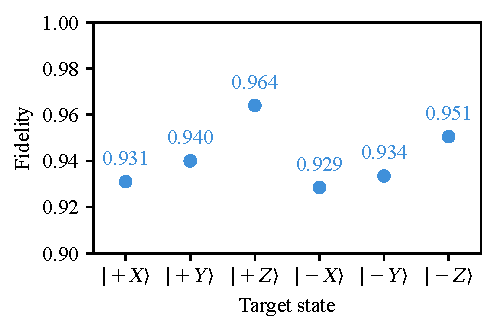
\includegraphics[width=0.6\linewidth]{figures/local-tomography.pdf}
%     \caption{
%         Average fidelity of the prepared cardinal states $\ket{+X}$, $\ket{+Y}$, $\ket{+Z}$,
%         $\ket{-X}$, $\ket{-Y}$, and $\ket{-Z}$ in the local qubit state tomography application.
%     }
%     \label{fig:local-tomo}
% \end{figure}

\subsection{Entanglement Generation}

The second test case is an application that generates an entangled pair between two nodes and then
measures the generated state. This is a distributed application, where both nodes are active ---
they engage in entanglement generation, and they both measure their end of the entangled pair. As
the user can specify the requested fidelity of the entangled pairs, this application is to be run
for various target fidelities. This time, all \acrshort{qnodeos} components are at work. Since
entanglement is requested, the quantum network stack is triggered, and thus the network process
becomes active, competing for resources with the user process. The \acrshort{qmmu} is also invoked
by the network process to transfer ownership of the entangled qubit to the user process (the
inter-process communication primitive of \acrshort{qnodeos}).

\paragraph{Configurations and expected results}

Entanglement generation is run for a range or target fidelities: \numlist{0.50; 0.55; 0.60; 0.65;
0.70; 0.75; 0.80}. Entangled pairs are read out in various bases to measure their correlators
$\braket{\mathrm{XX}}$, $\braket{\mathrm{YY}}$ and $\braket{\mathrm{ZZ}}$ (and their $\pm$
variations, for a total of $12$ correlators). The application is run \num{125} times for each
combination of target fidelity and correlator, for a total of \num{10500} entangled pairs. We expect
the measured fidelity to be at least matching --- within measurement uncertainty --- the requested
minimum fidelity, if the quantum hardware is capable of delivering such requested fidelities.

% The results for measured fidelity versus requested fidelity are shown in \cref{fig:ent-gen}. The
% measured fidelities are --- within measurement uncertainty --- always matching or exceeding the
% requested minimum ones (the dashed gray line in \cref{fig:ent-gen} is the $y=x$ diagonal). It is to
% be noted that measurement outcomes are post-processed to eliminate tomography errors and events in
% which the physical devices were in the incorrect charge state.
%
% \begin{figure}[t]
%     \centering
%     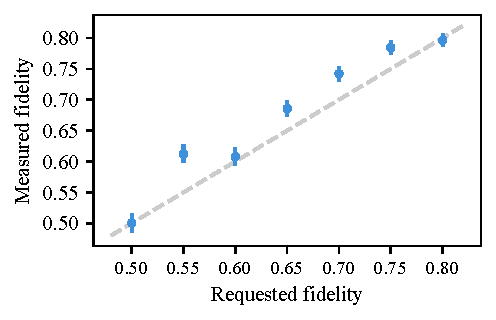
\includegraphics[width=0.6\linewidth]{figures/ent-gen.pdf}
%     \caption{
%         Measured fidelity of the entangled states generated and read out via \acrshort{qnodeos}.
%         Measurements are corrected to eliminate tomography errors and events in which the physical
%         devices were in the incorrect charge state. Error bars represent 1 s.d. The dashed gray line
%         is the $y=x$ diagonal.
%     }
%     \label{fig:ent-gen}
% \end{figure}

\subsection{Delegated Computation}

With this case study we aim to showcase a more complex quantum network application, schematically
depicted in \cref{fig:del-comp}. Here, one node acts as the client, and the other as the server. The
client's goal is to delegate a certain quantum computation on some data qubit to the server, while
keeping the server agnostic to the computation. To perform the desired computation, described by a
parameter $\alpha$, the two nodes follow these steps:
%
\begin{inlinelist}
    \item the two node establish an entangled pair,
    \item the client ``encodes'' its qubit by means of a series of local gates, described by a
          parameter $\theta$,
    \item the client measures its end of the entangled pair and stores the classical outcome
          $m_\text{c}$
    \item the client communicates the delegated computation parameter, which is a function of
          $\alpha$, $\theta$ and $m_\text{c}$,
    \item the server performs the computation,
    \item the server measures its end of the entangled pair and sends the classical outcome
          $m_\text{s}$ back to the client.
\end{inlinelist}
In this scheme, the client application consists of a single quantum code block and an additional
classical code block that communicates the computation parameter to the server. More interestingly,
the server application comprises two quantum code blocks --- the first is the establishment of the
entangled pair, and the second is the delegated computation --- interleaved by a classical code
block that receives the computation parameter from the client. This is the first example of an
application with inter-block and inter-node data dependencies, where the execution (on the server)
spans more than one quantum code block, and thus the quantum state generated in one block has to
persist and remain valid for the other block too.

\begin{figure}[t]
    \centering
    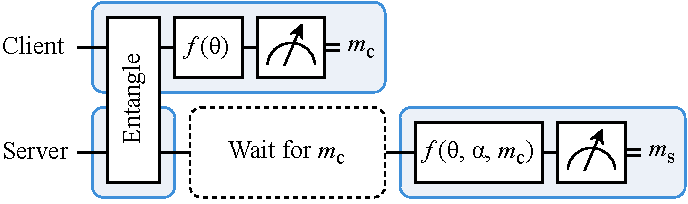
\includegraphics[width=0.6\linewidth]{figures/del-comp.pdf}
    \caption{
        Schematic of delegated computation application. The client wishes to have the server perform
        a quantum computation on a certain data qubit. To do so, the two nodes establish
        entanglement, then the client processes and measures its end of the entangled pair, sends
        the computation parameter to the server, which finally executes the delegated computation.
        Blue boxes represent quantum code blocks. The client's application is composed of a single
        block, while the server's consists of one block for entanglement and one block for the
        quantum computation, interleaved by a classical code block (the reception of the computation
        parameter).
    }
    \label{fig:del-comp}
\end{figure}

\paragraph{Configurations and expected results}

The delegated computation is run for various values of $\alpha$ ($\pi$, $\pi/2$) and $\theta$
($\pi$, $\pi/2$, $\pi/4$). The application is run \num{500} times for each combination of $\alpha$
and $\theta$. The metrics of interest are:
%
\begin{inlinelist}
    \item the measured fidelity of the qubit state after the delegated computation for each of the
          computation values,
    \item a breakdown of the average application latency, to give an indication of where time is
          spent during execution.
\end{inlinelist}
We expect the fidelity to be somewhat lower than the best-case performance due to the communication
latency incurred at the application level --- the ``Wait for $\theta, \alpha, m_c$'' block in
\cref{fig:del-comp}. In the latency breakdown, we also expect this classical communication step at
the application level to be the dominating factor. These delays are expected to manifest in
distributed applications. The resulting idle times can be allocated to other pending applications.

% We report the measured fidelity of the qubit state after the delegated computation for each of the
% computation values. We also report a breakdown of the average application latency, to give an
% indication of where time is spent during execution. \note{Plot and discuss data} The abstractions
% provided by \acrshort{qnodeos} allow for the execution of more complex quantum network applications.
% Distributed applications may result in idle time on some nodes, which \acrshort{qnodeos} can
% allocate to other pending applications.

\subsection{Multitasking}

One of the core features of modern \acrshortpl{os} is the ability to run several applications
concurrently, a key aspect in multi-user nodes and networks. \acrshort{qnodeos} is designed with
multitasking capabilities --- not only can it multiplex a user process and the network process, but
it also allows for multiple user processes to run at the same time. This means that multiple users
can submit their applications simultaneously, and \acrshort{qnodeos} will service all pending user
processes based on resource availability, in order to increase the utilization of the
\acrshort{qdevice} and to limit idle time and average application latency. One possible shortcoming
of multitasking on a quantum network node is the trade-off between concurrency and fidelity:
applications that have active data in the quantum memory, and that are waiting to be scheduled while
other applications are in progress, may experience lower-quality qubit states, given that such
quality degrades due to the passing of time and to the noise induced by operations on other qubits.

We aim to demonstrate the multitasking capabilities of \acrshort{qnodeos} by having multiple users
run independent applications concurrently. In our case study, a pool of users runs the delegated
computation application, while the rest of the users runs the local single-qubit gate tomography
application. Multitasking is evaluated on the client node, while the server just runs its part of
the delegated computation application. The idle time resulting from running the delegated
computation application on the client is a perfect candidate for scheduling other pending
applications. The multitasking performance of \acrshort{qnodeos} is assessed under various system
load conditions, which essentially depend on the number of users submitting applications
\acrshort{qnodeos} at the same time. We note that, even though a higher degree of concurrency should
in principle results in better device utilization, this is limited by the scarce physical resources
available on the underlying \acrshort{qdevice}.

\paragraph{Configurations and expected results}

Device utilization and average application latency are measured on the client, for various
configurations of users and applications: $N$ users, with $N \in \{2, 3, 5, 10\}$, half (rounded up)
of which running the local single-gate tomography application, and the remaining half (rounded down)
running the delegated computation application. To measure the performance benefit of multitasking,
we also run the same set of applications with multitasking disabled --- on \acrshort{qnodeos}, this
means that a user process can only be scheduled if no other user processes are either running or
waiting for entanglement generation. We expect the fidelity of the states measured at the end of
both applications to be somewhat comparable across the configurations with and without multitasking
enabled, given that the underlying \acrshort{qdevice} has a one-qubit memory at the moment, and thus
the level of concurrency is fairly limited. On the other hand, we expect device utilization and
average application latency to be affected by the multitasking capabilities of \acrshort{qnodeos}.
Whilst this is a relatively simple benchmark and the degree of concurrency is highly limited by the
available quantum memory, this case study should exemplify why it is important for an \acrshort{os}
for quantum network nodes to be multitasking-capable, and how such an \acrshort{os} can take
advantage of idle times.

% We report device utilization and average application latency, for the various usage patters,
% resulting from a continuous execution of each usage pattern over \qty{\approx 30}{min}. \note{Plot
% and discuss data} The scheduler of \acrshort{qnodeos}, in combination with the \acrshort{qmmu}, can
% dynamically re-prioritize outstanding processes based on resource availability. \acrshort{qnodeos}
% can thus support multi-user quantum network nodes, and can take advantage of network idle times to
% improve device utilization and average application latency. Impact of multitasking on fidelity not
% visible with a single qubit.

\section{Discussion}

The test cases discussed in this chapter complement those of \cref{chp:netstack}, and represent a
milestone for the evaluation of \acrlongpl{os} for quantum network nodes. These experiments are
planned for \acrshort{qnodeos} for the near future. The results of this experimental effort will
primarily showcase certain aspects of the importance of software abstractions for quantum
networking. Additionally, the outcome will provide insights into design and implementation strengths
an pitfalls on \acrshort{qnodeos}, and establish a baseline performance for similar studies
involving future versions of our system or alternative designs.

In the next and final chapter of this thesis we analyze the impact of \acrlong{doa} of classical
messages exchanged at the quantum network stack level. The results of this investigation will serve
as guidelines for incorporating \acrlong{doa} mechanisms into more advanced designs of
\acrshort{qnodeos}.

\begin{xstretch}
\printbibliography[heading=subbibintoc,title={References},notcategory=noprint]
\end{xstretch}

\chapter{Data Origin Authentication in the Quantum Networking Stack}
\label{chp:doa}

\begin{abstract}
Typically, quantum networking protocols make use of classical communications to coordinate
entanglement generation and other tasks. In this chapter, we discuss the need for authentication of
such classical messages exchanged at the quantum network stack level, with focus on concrete
protocol proposals. We then experimentally measure the overhead incurred by sending authenticated
classical messages through an authentication system that uses key material supplied by an
\acrshort{mdiqkd} system. We use this information to simulate the performance of a quantum link
whose protocol stack uses an authenticated classical channel, and compare that to existing
simulations of the same protocol stack. We find that message authentication overhead is not
detrimental to entanglement requests that end with an immediate measurement of the qubit, but has a
much more pronounced effect on entanglement requests that require storing the entangled qubit in
memory, and thus must be carried out sequentially.
\end{abstract}

\noindent
\note{This chapter is extracted from the data origin authentication paper. There aren't any major
additions.}

\blfootnote{
    This chapter is based on the preprint \fullcite{abrahams_2023_doa_noprint}. \note{Add proper
    link to arXiv when submitted}
}

\newpage

\lettrine{U}{p} until now, several proposals have been put forward as to how quantum networks should
be structured~\cite{van_meter_2013_repeaters, schoute_2016_shortcuts, joshi_2020_trusted}.
Researchers are also investigating how to abstract the complex physics of quantum networking so as
to provide platform-independent services to the end user~\cite{dahlberg_2019_egp,
pirker_2019_quantum, illiano_2022_quantum} --- the most basic of services being \emph{entanglement
generation}. One proposal for a \emph{quantum network stack} provides an outline of the layers and
separation of responsibilities, as well as protocols to populate these
layers~\cite{dahlberg_2019_egp, kozlowski_2020_qnp}. Within the proposed stack, each layer makes use
of the service exposed by the layer below, and provides a higher-level service to the layer
above~\cite{dahlberg_2019_egp}. This stack is inspired by the well-known \acrshort{tcpip} stack for
classical networks, and is illustrated in \cref{fig:functional-allocation}. Each protocol within the
quantum network stack makes use of classical control messages, exchanged over a classical network,
to coordinate quantum communication activities. These messages together form what we refer to as the
\emph{classical data plane} --- which lives alongside the \emph{quantum data plane}, where
information encoded in the quantum system is transmitted.

\begin{figure}[b]
    \centering
    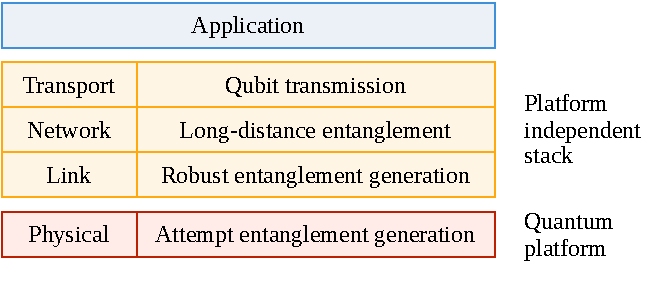
\includegraphics[width=0.6\linewidth]{figures/functional-allocation.pdf}
    \caption{
        Functional allocation of layers in a quantum network stack, adapted from
        Ref.~\cite{dahlberg_2019_egp}. The physical layer is quantum platform-dependent. The link
        layer provides platform-independent robust entanglement generation. All subsequent layers
        are therefore also platform independent, including the network and optionally transport
        layers which facilitate end-to-end entanglement between non-adjacent nodes. The application
        layer uses the services offered by the stack to perform quantum networking tasks.
    }
    \label{fig:functional-allocation}
\end{figure}

Such classical messages must be transmitted in a secure manner for a quantum network to function
reliably. \citeauthor{satoh_2020_attacking} mention forged classical messages as a general concern
for quantum networks~\cite{satoh_2020_attacking}. To prevent such forgeries, quantum network nodes
may employ \acrfull{doa}, to distinguish between genuine and fraudulent classical messages.
\acrshort{doa} is performed using a secret which is shared between two parties. A \acrfull{mac}
produces a tag for each message both at the sending and at the receiving end, to verify that the
message contents
%
\begin{inlinelist}
    \item were not altered and
    \item were produced by a party which owns the shared secret.
\end{inlinelist}
%
This structure is illustrated in \cref{fig:mac-structure}.

\begin{figure}[t]
    \centering
    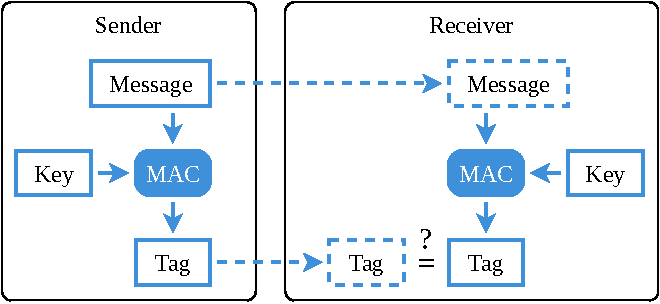
\includegraphics[width=0.6\linewidth]{figures/mac-structure.pdf}
    \caption{
        General structure of a \acrfull{mac}, where sender and receiver have a shared key. The
        receiver checks the output of the \acrshort{mac} to verify that the message was not modified
        in transit.
    }
    \label{fig:mac-structure}
\end{figure}

When designing control protocols for quantum networks, one should carefully estimate their impact on
end-to-end entanglement generation latency. Besides the more obvious reasons to do so, there is a
fundamental aspect of quantum information that imposes strict constraints on end-to-end latency:
storing quantum data reliably for extended periods of time is non-trivial. Qubits have relatively
short lifetimes, usually of the order of milliseconds, or at best of a few
seconds~\cite{abobeih_2018_one_sec, bradley_2019_one_min}. Therefore, not only can high end-to-end
latency affect the quality of the service offered by the network, but in some cases it may result in
no service at all. Classical processing and communication overhead must, thus, be kept to a minimum,
such that the entangled qubits can be used as quickly as possible.

Inevitably, performing \acrshort{doa} on messages exchanged in the classical data plane would incur
some computation and communication overhead. Such overhead is typically neglected when modeling,
simulating, or experimentally validating network protocols for quantum communications. In this work,
we illustrate the effects of classical authentication on a hypothetical quantum link. We first
experimentally measure the delays incurred by \acrshort{doa}, when performed on a sample of
classical messages using a \acrshort{qkd}-powered authentication proxy. We then analyze the behavior
of the hypothetical quantum link --- using a simulator for quantum
networks~\cite{coopmans_2021_netsquid} --- where the model of the classical communication channel of
such setup includes the measured classical delays incurred by \acrshort{doa}. The contributions of
this work are as follows:

\begin{enumerate}
    \item We provide a concise motivation for why \acrshort{doa} is a necessary component to uphold
          the availability of system-level protocols of the quantum network stack, and to help
          maintain the integrity of quantum data.
    \item We experimentally measure the delays incurred by \acrshort{doa}, performed using a
          \acrshort{qkd}-based authentication system, when run on a classical communication link.
    \item We offer a quantitative analysis of the impact of \acrshort{doa}, using the delays
          measured as per the previous point, when applied to the quantum network protocols of a
          hypothetical quantum link, as introduced in Ref.~\cite{dahlberg_2019_egp}.
\end{enumerate}

\section{Related Work}
\label{sec:doa:relwork}

Classical networking is an essential component of quantum networks and quantum networking
applications. \citeauthor{kozlowski_2019_towards} mention that the security of classical
communications is of concern when designing a quantum network~\cite{kozlowski_2019_towards}.
\citeauthor{satoh_2020_attacking} present a general motivation for authenticating the classical
channel of a quantum link~\cite{satoh_2020_attacking}. They model attack vectors on quantum
communications through the lens of \acrfull{cia}. Without any security measures in place, an
attacker may:

\begin{itemize}
    \item Disrupt the network in any number of ways, affecting its \emph{availability}.
    \item Interfere with data sent via the network, hampering the \emph{integrity} of quantum data.
    \item Read quantum data through the accompanying classical data, affecting
          \emph{confidentiality}.
\end{itemize}
Even though the confidentiality of quantum data itself is solely the responsibility of the
application layer (\cref{fig:functional-allocation}), privacy concerns such as \emph{tracking} are
still an issue if an attacker can read all classical communication.

All proposals of quantum network designs and quantum network protocols identified use some form of
classical communication to coordinate quantum communication and
entanglement~\cite{van_meter_2013_repeaters, schoute_2016_shortcuts, joshi_2020_trusted,
pirker_2019_quantum, kozlowski_2019_towards, dahlberg_2019_egp, kozlowski_2020_qnp}. We investigate
one such proposal for a quantum network stack, the one put forth by \textcite{dahlberg_2019_egp},
which has been evaluated in simulation, as well as on hardware~\cite{pompili_2022_experimental}
(\cref{chp:netstack}), and extended by \textcite{kozlowski_2020_qnp}.

The proposed protocol stack for quantum networks includes physical, link, network, transport, and
application layers, as illustrated in \cref{fig:functional-allocation}. The physical layer protocol,
called \acrfull{mhp}~\cite{dahlberg_2019_egp}, performs heralded entanglement generation attempts,
replying using a single repeater station. At the link layer, the
\acrfull{qegp}~\cite{dahlberg_2019_egp} has an internal retry mechanism and performs coordination
between adjacent nodes to provide more robust entanglement generation. \acrshort{qegp} accepts two
types of requests from the layer above:
%
\begin{inlinelist}
    \item \acrlong{ck} (\acrshort{ck}), to create an entangled pair and store it in memory;
    \item \acrlong{md} (\acrshort{md}), to create entangled pair, measure it, and report is outcome.
\end{inlinelist}
At the network layer, the \acrfull{qnp}~\cite{kozlowski_2020_qnp} coordinates entanglement
generation and swap operations on the full chain of intermediate nodes between two non-adjacent end
nodes.

We analyze the three service-level protocols \acrshort{mhp}, \acrshort{qegp}, and \acrshort{qnp},
and illustrate why \acrfull{doa} is important for these protocols to function, mostly with regards
to \emph{availability} of the network, and \emph{integrity} of quantum data.

\section{Why Data Origin Authentication}
\label{sec:doa:why}

We investigate the applicability of \acrlong{doa} to three system-level protocols for quantum
network stacks: \acrshort{mhp}, \acrshort{qegp} and \acrshort{qnp}~\cite{dahlberg_2019_egp,
kozlowski_2020_qnp}. Quantum application protocols (e.g. \acrshort{qkd}) lie outside the scope of
this work. Here, we provide a non-exhaustive list of example actions that a malicious actor may
perform if they are allowed to forge or modify classical messages exchanged at the protocol level.
We mention whether each action affects the \emph{availability} of the link or network, or the
\emph{integrity} of the quantum data sent via the network.

\paragraph{Physical layer}

\acrshort{mhp} operates at the physical layer. Hardware vulnerabilities of the physical entanglement
generation process are outside the scope of this work.

\begin{example}
\textit{Availability.}
Change a successful heralding signal to an error code such Alice and Bob falsely conclude that
entanglement has failed.
\end{example}

\begin{example}
\textit{Integrity.}
Modify the heralding signal from the midpoint station by changing the state announcement such that
Alice or Bob apply the wrong Pauli corrections to their qubits.
\end{example}

\begin{example}
\textit{Integrity.}
Interfere with mismatch verification~\cite{dahlberg_2019_egp, pompili_2022_experimental} such that
Alice and Bob falsely conclude that a \acrshort{mhp} request belongs to the same \acrshort{qegp}
request, thus hampering the integrity of quantum data due to cross-process interference.
\end{example}

\paragraph{Link layer}

\acrshort{qegp} operates at the link layer~\cite{dahlberg_2019_egp}. As proposed in
Ref.~\cite{dahlberg_2019_egp}, it is used to synchronize entanglement requests, and to communicate
the number of available memory qubits and the expiration of requests.

\begin{example}
\textit{Availability.}
Continually send requests for entanglement, exhausting the resources of nodes receiving
them~\cite{kozlowski_2019_towards}.
\end{example}

\begin{example}
\textit{Availability.}
When advertising the number of available communication or storage qubits, set either to 0. The
receiving node then assumes that there are no communication or storage qubits available on the
sending node.
\end{example}

\begin{example}
\textit{Integrity.}
Change the qubit identifier of an entanglement generation request such that Alice and Bob entangle
the wrong data qubits, causing cross-path or process interference.
\end{example}

\paragraph{Network layer}

\acrshort{qnp} operates at the network layer. Conceptually, it allows non-adjacent nodes in a
quantum network to coordinate entanglement generation. This is akin to the \acrfull{ip} in the
classical stack. It makes use of \texttt{FORWARD} and \texttt{TRACK} messages to track entanglement
generation~\cite[Figure 6]{kozlowski_2020_qnp}. \texttt{FORWARD} messages are used to communicate
entanglement requests, and \texttt{TRACK} messages contain classical correction information for both
end-nodes in the network.

\begin{example}
\textit{Availability.}
Modify \texttt{FORWARD} message so that intermediary nodes do not receive entanglement swap
instructions.
\end{example}

\begin{example}
\textit{Integrity.}
Modify \texttt{TRACK} messages such that the end-nodes of a path do not receive the correct
entanglement swap outcome, and thus apply the wrong corrections to their qubits.
\end{example}

\begin{figure}[t]
    \centering
    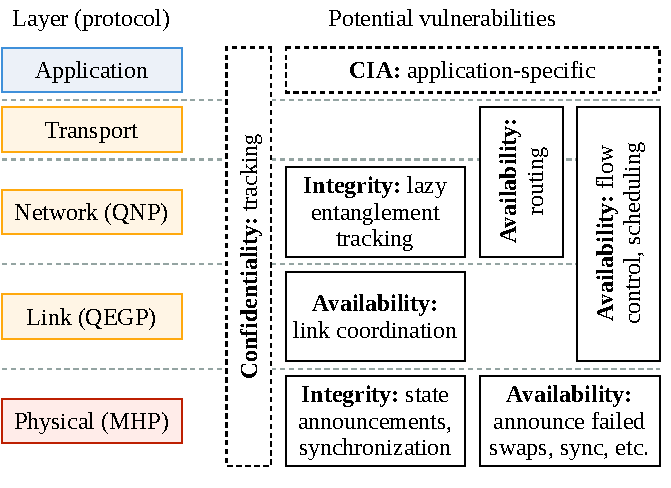
\includegraphics[width=0.6\linewidth]{figures/doa-examples.pdf}
    \caption{
        Example effects of tampering with control messages at each layer of the quantum network
        stack through the lens of \acrfull{cia}. We take as examples concrete implementations of
        quantum network protocols --- including \acrshort{qnp}, \acrshort{qegp} and
        \acrshort{mhp}~\cite{kozlowski_2020_qnp, dahlberg_2019_egp} --- to highlight the potential
        vulnerabilities at each layer. In this work, we do not focus on confidentiality issues (see
        Ref.~\cite{satoh_2020_attacking}).
    }
    \label{fig:doa-examples}
\end{figure}

We illustrate the concerns of availability and data integrity in a quantum network stack in
\cref{fig:doa-examples}. Such security threats are addressed in part by using \acrlong{doa}, which
can prevent modification and forgery of classical control messages. It should be noted, however,
that availability may still be hampered by an adversary capable of halting transmission of classical
control messages outright. Furthermore, if a malicious actor were to gain access to a node itself
then this might circumvent many or all security mechanisms in place, including \acrshort{doa}, and
should therefore also be prevented.

More in general, we also note that classical control messages might reveal information about who is
using the network and the types of operations being performed. Therefore, in a more mature network,
it will likely be worthwhile to also encrypt the contents of control messages.
\citeauthor{satoh_2020_attacking} mention tracking as a general concern for inter-node classical
communication within the quantum stack~\cite{satoh_2020_attacking}. Encryption combined with
transmission of random noise could address tracking concerns.

\section{Experimental Methodology}
\label{sec:doa:meth}

We aim to illustrate the effects of \acrlong{doa}, and the total overhead incurred by classical
control messages, on the performance of a hypothetical quantum link. To limit the scope of our
investigation, we focus on the performance of link and physical layer protocols as proposed by
\textcite{dahlberg_2019_egp}, and we extend the simulation therein such that it fully models
%
\begin{inlinelist}
    \item classical transmission overhead and
    \item \acrshort{doa} overhead.
\end{inlinelist}

Instead of modeling communication overhead analytically, we measure it experimentally by recording
\acrfull{rtt} of sample control messages sent and authenticated through a full-blown data
authentication proxy. The proxy tags classical messages using key material obtained from a
\acrfull{mdiqkd} key server, based on the work by \textcite{berrevoets_2022_deployed}. We then
inject the measured overhead into the simulation parameters, and then extract performance metrics as
done in Ref.~\cite{dahlberg_2019_egp}. The process of measuring classical communication overhead is
explained in \cref{sec:doa:latency}, while the simulation results are presented in
\cref{sec:doa:results}.

\section{Measuring Classical Latency}
\label{sec:doa:latency}

In order to obtain an estimate of the expected latency incurred by classical control messages in a
quantum network stack, we measure the \acrfull{rtt} of a sample of messages when sent through an
authenticated classical channel in the field. The messages are \acrshort{icmp} (ping) packets, sized
to mimic \acrshort{qegp} and \acrshort{mhp} packets. The authentication mechanism is external to the
nodes exchanging ping messages, acting as a proxy between them. The proxy's \acrshort{mac}
calculates a tag over the sent message, transmits the message and the tag, and verifies the tag at
the receiving end before delivering the message to the destination node. The experimental setup is
depicted in \cref{fig:mac-setup-diagram}.

Ping messages are exchanged between two real-time classical network nodes similar to those used in
the experimental validation of \acrshort{qegp}~\cite{pompili_2022_experimental}
(\cref{chp:netstack, chp:qnodeos}) --- MicroZed boards~\cite{microzed} running a
FreeRTOS~\cite{freertos} application --- connected to the proxy via a Gigabit Ethernet interface.
The source node records the \acrshort{rtt} of the message, and computes various statistics on these
timestamps, most notably average and standard deviation. We use these statistics to extrapolate the
expected classical communication latency for the various simulation scenarios presented in
\cref{sec:doa:results}.

The \acrfull{mac} on both ends retrieves authentication keys from a local key server, which contains
key material identical to its counterpart at the other end. Key material is produced by an
\acrshort{mdiqkd} implementation deployed in the Utrecht area, in the Netherlands. The
\acrshort{mdiqkd} system is very similar to the one implemented in
Ref.~\cite{berrevoets_2022_deployed}, though with a few differences. Firstly, the upgraded system
uses a four-intensity decoy state protocol~\cite{zhou_2016_making, woodward_2021_gigahertz}, which
improves key rate. This is an improvement over the three-intensity decoy state
protocol~\cite{yu_2013_three} of the previous deployment. Second, there are now separate, dedicated
fiber-optic cables for quantum and classical messages. In the original system these were combined,
at the cost of reduced key rate.

\begin{figure}[t]
    \centering
    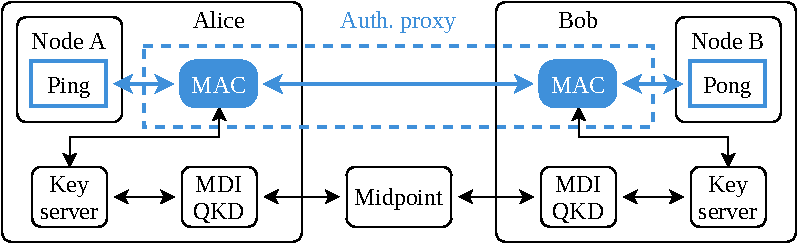
\includegraphics[width=0.6\linewidth]{figures/mac-setup-diagram.pdf}
    \caption{
        Experimental setup used to measure the end-to-end delays of transmitting an
        \emph{authenticated classical message} from Alice to Bob with \qty{42}{\km} of fiber-optic
        cables between them. Classical messages go through an authentication proxy that tags
        messages using \acrshort{mdiqkd}-generated key material.
    }
    \label{fig:mac-setup-diagram}
\end{figure}

\paragraph{Authentication proxy configuration}

We collect classical communication latency measurements under four different configurations of the
authentication proxy:

\begin{enumerate}
    \item Bypass proxy: at first, we bypass the authentication proxy altogether. This is useful to
          measure baseline communication latency, excluding all computation delays that would be
          introduced by the proxy.
    \item No \acrshort{mac}: this time, the proxy is configured to skip the authentication (and
          verification) step, but packets do go through the proxy's processing pipeline. Results for
          this configuration give us insights into the overhead of processing packets on the proxy,
          excluding the computation latency incurred by the \acrshort{mac} authentication (and
          verification) step.
    \item \acrshort{vmac}: in this configuration, the proxy computes and verifies message tags using
          the information-theoretically secure \acrshort{vmac} scheme~\cite{krovetz_2007_message}.
          We use both standard \acrshort{vmac} and a modified version that uses 21-bit tags
          (\acrshort{vmac}-21) instead of the default 64-bit tags.
    \item \acrshort{poly}: finally, we configure the proxy to use the computationally secure
          \acrshort{mac} called \acrshort{poly}~\cite{bernstein_2005_poly1305}. As opposed to
          \acrshort{vmac}, \acrshort{poly} can reuse the same key material for multiple messages.
\end{enumerate}

\paragraph{Rate and size of messages}

With the current implementation of the authentication proxy, one cannot transmit a classical message
more than once every \qty{10}{\ms} without experiencing detrimental packet loss. This contrasts with
the assumption in Ref.~\cite{dahlberg_2019_egp}, where \acrshort{mhp} messages are sent at a rate up
to \qty{100}{\kHz}. To circumvent this, we assume that \acrshort{mhp} messages may be batched
together and transmitted as part of a larger packet, and thus transmit ping messages at a rate of
\qty{100}{\Hz}.

Moreover, the current implementation of the proxy can only authenticate packets with a payload that
is small enough to be accommodated --- together with all protocol headers and the \acrshort{mac} tag
--- in a single Ethernet frame. Therefore, we send ping messages with payloads of
%
\begin{inlinelist}
    \item \num{12}~bytes, which is the size of the smallest \acrshort{qegp} message, and
    \item \num{1200}~bytes, which is close to the maximum allowed by the proxy.
\end{inlinelist}

\paragraph{Network topology}

The link connecting Alice to the center node runs for \qty{20}{\km}, whereas the link between Bob
and the center node is \qty{22}{\km} in length. Thus, the \acrshort{rtt} we measure is for a link of
a total length of \qty{42}{\km}. The topology of Alice, Bob, and the center node of the
\acrshort{mdiqkd} system is illustrated in \cref{fig:mac-setup-qkd-locations}.

\begin{figure}[t]
    \centering
    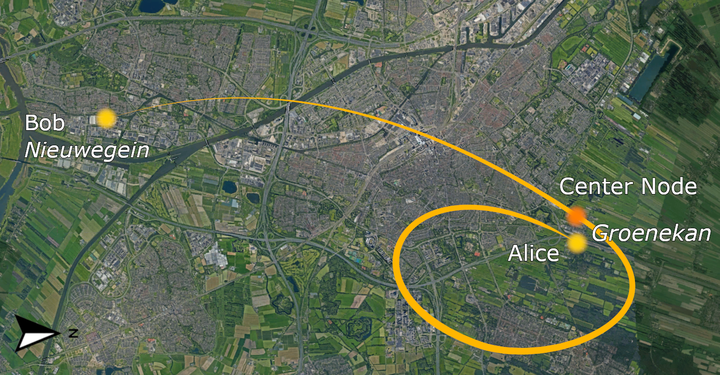
\includegraphics[width=0.6\linewidth]{figures/mac-setup-qkd-locations-resized.png}
    \caption{
        Physical layout of Alice and Bob nodes. Alice is located in Groenekan, the Netherlands,
        while Bob is in Nieuwegein, the Netherlands. The optical fiber connecting Alice to the
        center node is \qty{20}{\km} in length, whereas the connection between Bob and the center
        node is \qty{22}{\km}.
    }
    \label{fig:mac-setup-qkd-locations}
\end{figure}

\paragraph{Results}

We record the \acrlong{rtt} of \num{360000} ping messages per configuration (proxy configuration and
size of message). The computed mean and standard deviation of the results are reported in
\cref{tab:rtt}.

When bypassing the proxy altogether, the mean \acrshort{rtt} (less than \qty{4}{\ms}) is dominated
by propagation and transmission time through the experimental network. The small standard deviation
suggests that this baseline latency is quite stable. When messages go through the authentication
proxy but are not authenticated, the mean \acrshort{rtt} increases by a factor of around \num{3.5},
and the standard deviation becomes non-negligible. This is an indicator of the poor packet
processing performance of the proxy, which is merely a soft-processing packet pipeline implemented
in Python (the authentication proxy was designed for demonstration purposes, not performance). The
computational overhead introduced by the actual \acrshort{mac} is overshadowed by the baseline
latency of the proxy, as observed in the \acrshort{poly} configuration. Finally, statistics for the
\acrshort{vmac} configuration could not be computed at all, as far too many messages are dropped by
the proxy due to lack of key material. This is to be expected, given the high rate of key
consumption of the information-theoretically secure code. Interestingly, the size of messages does
not appear to be a noticeable factor in the mean end-to-end latency. We can therefore conclude that
latency is dominated by two main factors:
%
\begin{inlinelist}
    \item the length of the link, which depends on the network topology, and
    \item the packet processing performance of the proxy, which is approximately constant.
\end{inlinelist}

\section{Simulation Results}
\label{sec:doa:results}

We quantify the effects of using an authenticated classical channel for control messages exchanged
at the quantum network stack level. In particular, we augment the model used by
\textcite{dahlberg_2019_egp} to simulate the performance of physical (\acrshort{mhp}) and link
(\acrshort{qegp}) layer protocols within the quantum network stack. As opposed to the original work,
we model classical communication delays to also include transmission and authentication overhead,
when using \acrshort{poly} to authenticate messages, measured as described in
\cref{sec:doa:latency}. We report the \emph{throughput} of the quantum link, expressed as number of
entangled pairs generated per second.

\begin{table}
    \centering
    \begin{tabularx}{0.75\linewidth}{@{} lYYYY @{}}
        \toprule
        \textbf{Proxy}                     & \textbf{Tag size}          & \textbf{Payload} & \multicolumn{2}{c}{\textbf{\acrshort{rtt}} [\unit{\us}]}                 \\
        \cmidrule(l){4-5}
        \textbf{config}                    & [bits]                     & [Bytes]          & \textbf{mean}                                            & \textbf{std}  \\
        \midrule
        \multirow{2}{*}{Bypass proxy}      & \multirow{2}{*}{---}       & \num{12}         & \num{3656.61}                                            & \num{22.62}   \\
                                           &                            & \num{1200}       & \num{3881.37}                                            & \num{21.97}   \\
        \midrule
        \multirow{2}{*}{No \acrshort{mac}} & \multirow{2}{*}{---}       & \num{12}         & \num{13820.72}                                           & \num{3142.50} \\
                                           &                            & \num{1200}       & \num{13993.15}                                           & \num{2876.08} \\
        \midrule
        \multirow{2}{*}{\acrshort{poly}}   & \multirow{2}{*}{\num{128}} & \num{12}         & \num{14387.14}                                           & \num{5044.19} \\
                                           &                            & \num{1200}       & \num{13959.16}                                           & \num{2866.52} \\
        \midrule
        \acrshort{vmac}                    & any                        & any              & N/A                                                      & N/A           \\
        \bottomrule
    \end{tabularx}
    \caption{
        Mean and standard deviation of \acrfull{rtt} for different configurations of the proxy and
        for different message sizes. When using \acrshort{vmac}, most messages are dropped by the
        proxy due to lack of key material (resulting from the high rate of key consumption of
        \acrshort{vmac}), thus statistics are not available for that configuration.
    }
    \label{tab:rtt}
\end{table}

\paragraph{Configurations}

We run our simulations for two types of configurations:
%
\begin{inlinelist}
    \item To begin with, we study the performance of the link for several node-to-node distances, at
          a fixed requested fidelity ($F_\text{min}=0.65$). For the various distances, we scale the
          classical delays accordingly. For this configuration, we compare our augmented model with
          the original baseline, where transmission and authentication delays were not
          modeled~\cite{dahlberg_2019_egp}.
    \item Furthermore, we analyze quantum network throughput at a fixed node-to-node distance, but
          this time varying the requested fidelity at the \acrshort{qegp} layer. This time, we
          compare three models, corresponding to the three configurations of the proxy as per
          \cref{sec:doa:latency}: Bypass proxy, No \acrshort{mac}, and \acrshort{poly}. We do not
          report on \acrshort{vmac}, as we observed it requires more key material than our key
          server could supply (see \cref{sec:doa:latency}).
\end{inlinelist}

For each of the above configurations, we perform \num{20} simulation runs, each consisting of
\num{20} minutes of continuous use of the link. We then calculate the average throughput over all
runs for each configuration with a confidence interval of \qty{95}{\percent}.

\paragraph{Results}

\begin{figure}[t]
    \centering
    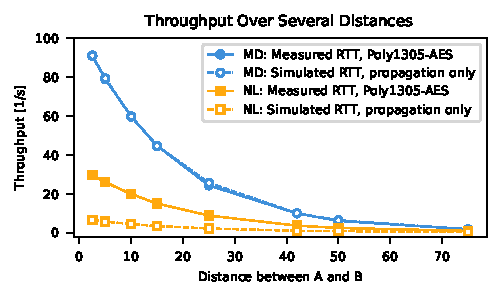
\includegraphics[width=0.6\linewidth]{figures/throughput_FCFS.pdf}
    \begin{tabularx}{0.6\linewidth}{@{} lYYYYYYYY @{}}
        \toprule%
                        & \multicolumn{8}{c}{\textbf{Breakdown of distance A -- B [\unit{\km}]}} \\%
        \midrule%
        \textbf{A -- M} & 1.5 & 3 & 6  & 9  & 15 & 22 & 30 & 45 \\%
        \textbf{M -- B} & 1   & 2 & 4  & 6  & 10 & 20 & 20 & 30 \\%
        \midrule%
        \textbf{Total}  & 2.5 & 5 & 10 & 15 & 25 & 42 & 50 & 75 \\%
        \bottomrule%
    \end{tabularx}%
    \caption{
        Throughput (rate) of entangled pair generation for multiple distances between node A and B,
        with a single midpoint station in between and for a requested fidelity of
        $F_\text{min}=0.65$. Classical communication delays were modeled using latency measurements
        collected as described in \cref{sec:doa:latency} (configuration ``\acrshort{poly}''), as
        well as replicated from the original simulations of \acrshort{qegp} and
        \acrshort{mhp}~\cite{dahlberg_2019_egp}. The table shows how distance is distributed between
        A, B, and the midpoint station. The \qty{25}{\km} data point is equivalent to the QL2020
        hypothetical setup simulated in Ref.~\cite{dahlberg_2019_egp}. The solid line represents
        mean throughput, the colored area around it depicts the \qty{95}{\percent} confidence
        interval.
    }
    \label{fig:results-distance}
\end{figure}

The results for throughput versus distance are illustrated in \cref{fig:results-distance}. For
\acrfull{md} type requests, mean throughput is approximately equal across the two models of
classical delays. This is to be expected, given that these types of requests can be pipelined, and
thus throughput is mostly dominated by the physical entanglement generation procedure, not as much
by classical communication latency. On the other hand, \acrfull{nl} requests --- which, for our
purpose, are equivalent to \acrfull{ck} requests --- show a more surprising outcome: the throughput
is higher for the configuration where classical communication models transmission authentication
delays on top of the propagation delays from the baseline~\cite{dahlberg_2019_egp}. We attribute
this effect to the fact that when classical communication is faster, \acrshort{qegp} request are
distributed at a faster rate, and thus the request queues fill up more quickly, resulting in a
higher request rejection rate. The discrepancy between our model and the baseline is especially
clear at shorter distances, where classical communication in the baseline model is considerably
faster than in our model.

The results for throughput versus fidelity are shown in \cref{fig:results-fidelity}. For this
experiment, the outcome just matches our expectations. \acrshort{md} requests are not affected by
classical communication much, and their throughput only decreases when higher-fidelity entangled
pairs are requested. \acrshort{nl} requests, instead, are more affected by classical communication
latency, and their throughput decreases more noticeably when classical messages go through the
authentication proxy. As expected from the results in \cref{tab:rtt}, the extra delays incurred by
the actual \acrshort{mac} computation are negligible, and their effect on throughput not noticeable.

\section{Discussion}

We have shown how the classical data plane of the quantum network stack presents a significant
attack surface for \acrlong{cia} of the quantum link and data. To address these concerns on must
employ, among other things, \acrlong{doa} on the classical control messages exchanged at the quantum
network stack level. We conclude that \acrlong{doa} is necessary to both uphold the integrity of
quantum data and the availability of the quantum network itself.

\begin{figure}[t]
    \centering
    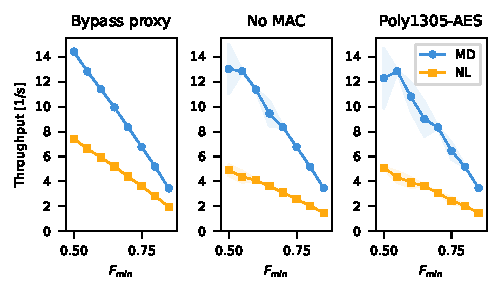
\includegraphics[width=0.6\linewidth]{figures/throughput_FCFS_mhp_150.pdf}
    \caption{
        Throughput (rate) of entangled pair generation for multiple requested fidelities, with
        \qty{20}{\km} between node A and the midpoint station, and \qty{22}{\km} between the
        midpoint station and node B, and for three configurations of the proxy as per
        \cref{sec:doa:latency}: Bypass proxy, No \acrshort{mac}, and \acrshort{poly}. \acrshort{vmac}
        results are omitted as packet drop rates are excessive. The solid line represents mean
        throughput, the colored area around it depicts the \qty{95}{\percent} confidence interval.
        \Acrfull{md} type requests are not as heavily affected as these are pipelined. \Acrfull{nl}
        type requests are performed sequentially, and thus increases in classical delays have a more
        profound impact on throughput.
    }
    \label{fig:results-fidelity}
\end{figure}

We have also simulated the performance of a hypothetical quantum link under the assumption that
classical messages were being authenticated in some sort of way. Here, we modeled classical
communication latency, including authentication overhead and transmission delay, using metrics
collected from a classical link authenticated using key material sourced from an \acrshort{mdiqkd}
system. If we disregard the large packet processing delays incurred by the authentication proxy used
in this work, we observe that an authenticated classical channel introduces a negligible amount of
extra classical overhead, provided that one uses an optimized \acrshort{mac}.

However, we have also seen that propagation and transmission delays themselves have a noticeably
negative effect on the performance of a quantum link, whether or not \acrlong{doa} is applied. While
the quantum link remains functional, the entanglement generation rate drops by a significant amount
for entanglement requests that do not end with an immediate measurement of the entangled qubit.

\printbibliography[heading=subbibintoc,title={References},notcategory=noprint]

\chapter{Conclusion}
\label{chp:conclusion}

\lettrine{M}{ost} interesting conclusions.

The conclusions of this thesis.

\printbibliography[heading=subbibintoc,title={References},notcategory=noprint]


% Use letters for the chapter numbers of the appendices.
\appendix

\chapter{QNodeOS Components and Interfaces}
\label{app:qnodeos}

We provide here additional details on the components of the \acrshort{qnodeos} architecture and
their intefaces. \Cref{fig:qnodeos-core} gives an overview of all the components of
\acrshort{qnodeos}. The \emph{process manager} marshals accesses to all user and kernel processes.
The \emph{scheduler} assigns ready processes to the \emph{processor}, which runs quantum
instructions through the underlying \acrshort{qdevice}, processes classical QASM instructions
locally, and registers entanglement requests with the \emph{\acrlong{emu}} (\acrshort{emu}). The
\acrshort{emu} maintains a list of EPR sockets and entanglement requests, forwards the latter to the
\emph{quantum network stack}, which, in turn, registers available entangled qubits with the
\acrshort{emu}. Finally, the \emph{\acrlong{qmmu}} (\acrshort{qmmu}) keeps track of used qubits, and
transfers qubit ownership across processes when requested.

\section{Process Manager}

The process manager owns \acrshort{qnodeos} processes and marshals accesses to those. Creating a
process, adding a routine to it and accessing the process's data must be done through the process
manager. Additionally, the process manager is used by other components to notify \emph{events} that
occur inside \acrshort{qnodeos}, upon which the state of one of more processes is updated. Process
state updates result in a notification to the scheduler.

\paragraph{Interfaces}

The process manager exposes interfaces for three services:
\begin{itemize}
    \item Process management (interface~\circled{1} in \cref{fig:qnodeos-core}): to create and
          remove processes, and to add routines to them. When the user registers an application, the
          \acrshort{qnodeos} \acrshort{api} Handler uses the process manager to create a
          \acrshort{qnodeos} user process. The returned process ID can be later used to add a
          routine to that process, or to remove the process once all its routines are fully
          processed.
    \item Event notification (interface~\circled{2} in \cref{fig:qnodeos-core}): to notify an event
          occurred inside \acrshort{qnodeos}, including the addition of a routine, the completion of
          a routine, the scheduling of the process, the hitting of a Wait condition, and the
          generation of an entangled qubit destined to the process. Some events trigger follow-up
          actions --- for instance, when a process that was waiting for an event becomes ready, it
          gets added to the queue of ready processes maintained by the scheduler.
    \item Process data access (interface~\circled{3} in \cref{fig:qnodeos-core}): to access a
          process's routines and its classical memory space, mostly used while running the process
          (through the processor).
\end{itemize}

\begin{figure}[t]
    \centering
    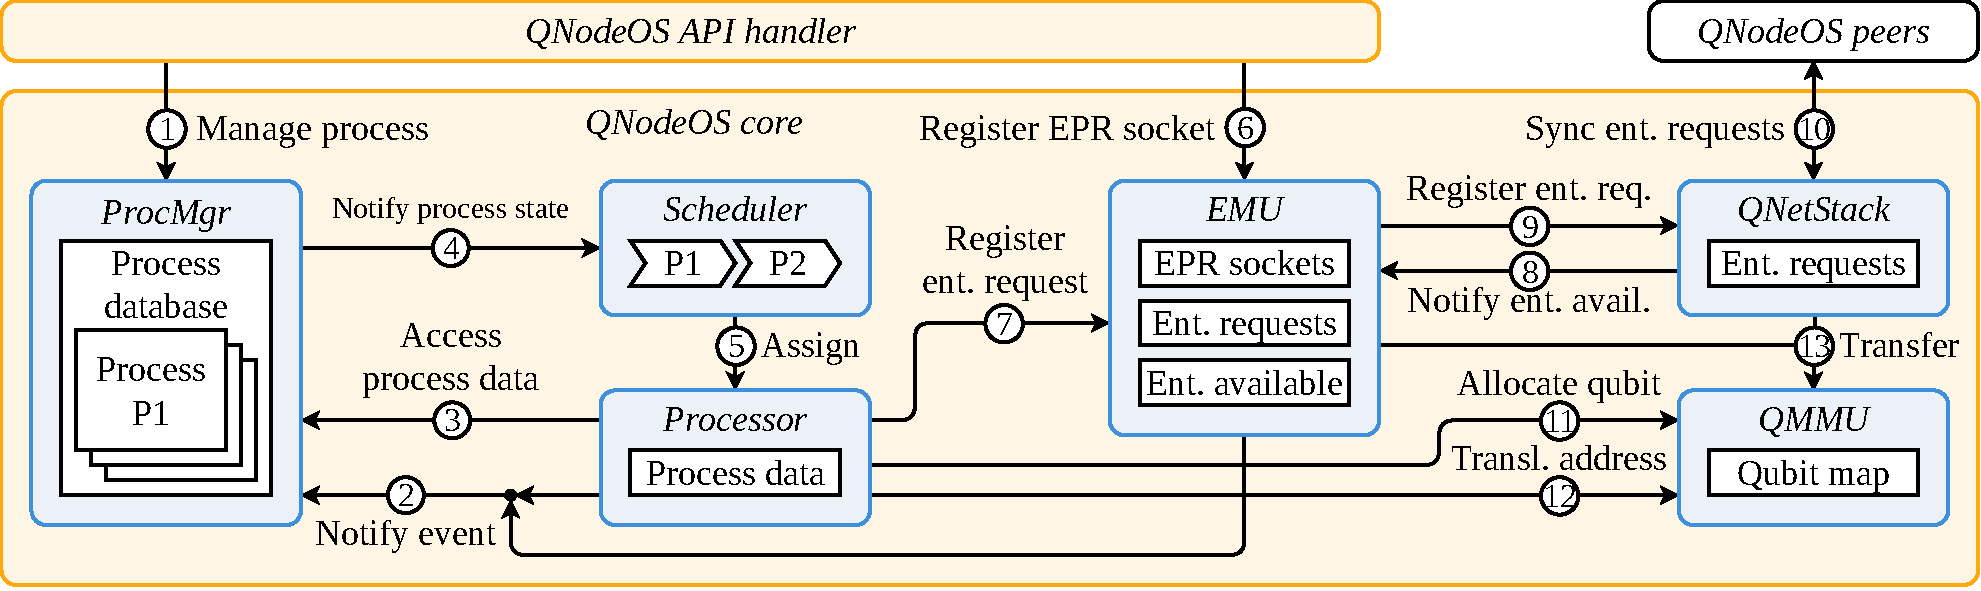
\includegraphics[width=\linewidth]{figures/qnodeos-core.pdf}
    \caption[]{
        \acrshort{qnodeos} core components and internal interfaces. The core layer includes:
        \begin{inlinelist}
            \item a \emph{process manager} (ProcMgr), which owns and manages access to
                  \acrshort{qnodeos} processes;
            \item a \emph{scheduler}, responsible for selecting the next process to be run;
            \item a \emph{processor}, which processes routines' instructions;
            \item an \emph{\acrlong{emu}} (\acrshort{emu}), which keeps a list of entanglement
                  requests and available entangled qubits;
            \item a \emph{quantum network stack} (QNetStack), whose responsibility is to coordinate
                  with peer nodes to schedule quantum networking instructions;
            \item a \emph{\acrlong{qmmu}} (\acrshort{qmmu}), which keeps a record of allocated
                  qubits.
        \end{inlinelist}
    }
    \label{fig:qnodeos-core}
\end{figure}

\section{Scheduler}

The \acrshort{qnodeos} scheduler registers processes that are ready to be scheduled, and assigns
them to the \acrshort{qnodeos} processor when the latter is available. Ready processes are stored in
a \emph{prioritized ready queue}, and processes of the same priority are scheduled with a
first-come-first-served policy.

\paragraph{Interfaces}

The scheduler only exposes one interface for process state notifications (interface~\circled{4} in
\cref{fig:qnodeos-core}), used by the process manager to signal when a process transitions to a new
state. When a \acrshort{qnodeos} process transitions to the ready state, it is directly added to the
scheduler's prioritized ready queue. When a process becomes idle, or is waiting for an event to
happen, the scheduler simply registers that the processor has become available.

\section{Processor}

The \acrshort{qnodeos} processor handles the execution of \acrshort{qnodeos} user and kernel
processes, by running classical instructions locally and issuing quantum instructions to the
\acrshort{qdevice} driver. While executing a process, the processor reads its routines and accesses
(reads and writes) its classical memory. The processor implements a specific instruction set
architecture dictated by the QASM language of choice.

\paragraph{Interfaces}

The processor exposes one interface for processor assignment (interface~\circled{5} in
\cref{fig:qnodeos-core}), used by the \acrshort{qnodeos} scheduler to activate the processor, when
it is idling, and assign it to a \acrshort{qnodeos} process.

\section{Entanglement Management Unit}

The \acrfull{emu} maintains a list of open \emph{EPR sockets} and a list of \emph{entanglement
requests}, and keeps track of the \emph{entangled qubits} produced by the quantum network stack.
Received entanglement requests are considered valid only if an EPR socket associated to such
requests exists. Valid requests are forwarded to the quantum network stack. Entangled qubit
generations are notified as events to the process manager.

\paragraph{Interfaces}

The \acrshort{emu} exposes interfaces for three services:
\begin{itemize}
    \item EPR socket registration (interface~\circled{6} in \cref{fig:qnodeos-core}): to register
          and open EPR sockets belonging to an application, and to set up internal classical network
          tables and to establish classical network connection.
    \item Entanglement request registration (interface~\circled{7} in \cref{fig:qnodeos-core}): to
          add entanglement requests to the list of existing ones, to be used when matching produced
          entangled qubits with a process that requested them.
    \item Entanglement notification (interface~\circled{8} in \cref{fig:qnodeos-core}): to register
          the availability of an entangled qubit, produced by the quantum network stack, and to link
          it to an existing entanglement request.
\end{itemize}

\section{Quantum Network Stack}

The quantum network stack on \acrshort{qnodeos} follows the model presented in
Ref.~\cite{dahlberg_2019_egp} which is based on the classical \acrshort{osi} network stack model for
separation of responsibilities. In particular, \emph{data link layer} and \emph{network layer}
protocols are part of the quantum network stack on \acrshort{qnodeos}. The \emph{physical layer} is
implemented on the \acrshort{qdevice}, the \emph{application layer} is part of the Host, and all
remaining layers are not currently part of the stack.

The quantum network stack component has an associated \emph{\acrshort{qnodeos} kernel process},
created statically on \acrshort{qnodeos}. However, this process's routine is dynamic: the
instructions to be executed on the processor depend on the outstanding entanglement generation
requests received from \acrshort{emu} and network peers.

\paragraph{Interfaces}

The quantum network stack exposes interfaces for two services:
\begin{itemize}
    \item Entanglement request registration (interface~\circled{9} in \cref{fig:qnodeos-core}): to
          add entanglement requests coming from the \acrshort{emu} to the list of existing ones,
          which are used to fill in the quantum network stack process's routine with the correct
          instructions to execute.
    \item Entanglement request synchronization (interface~\circled{10} in \cref{fig:qnodeos-core}):
          similar to the entanglement request registration interface, but to be used to synchronize
          (send and receive) requests with \acrshort{qnodeos} network peers.
\end{itemize}

\section{Quantum Memory Management Unit}

The \acrfull{qmmu} receives requests for \emph{qubit allocations} from \acrshort{qnodeos} processes,
and manages the subsequent usage of those. It also translates QASM \emph{virtual qubit addresses}
into physical addresses for the \acrshort{qdevice}, and keeps track of which process is using which
qubit at a given time. In general, a \acrshort{qmmu} should take into account that the topology of a
quantum memory determines what operations can be performed on which qubits, and thus allow processes
to allocate qubits of a specific type upon request. An advanced \acrshort{qmmu} could also feature
algorithms to move qubits in the background --- that is, without an explicit instruction from a
process's routine --- to accommodate an application's topology requirements while not trashing the
qubits being used by other \acrshort{qnodeos} processes. Such a feature could prove crucial to
increase the number of processes that can be using the quantum memory at the same time, and to
enhance multitasking performances.

\paragraph{Interfaces}

The \acrshort{qmmu} exposes interfaces for three services:
\begin{itemize}
    \item Qubit allocation and deallocation (interface~\circled{11} in \cref{fig:qnodeos-core}): a
          running process can ask for one or more qubits, which, if available, are allocated by the
          \acrshort{qmmu}, and their physical addresses are mapped to the virtual addresses provided
          by the requesting process.
    \item Virtual address translation (interface~\circled{12} in \cref{fig:qnodeos-core}): before
          sending quantum instructions to the \acrshort{qdevice} driver, the processor uses virtual
          qubit addresses specified in QASM to retrieve physical addresses from the \acrshort{qmmu},
          and then replaces virtual addresses with physical addresses in the instructions for the
          \acrshort{qdevice} driver.
    \item Qubit ownership transfer (interface~\circled{13} in \cref{fig:qnodeos-core}): qubits are
          only visible to the process that allocates them. However, in some cases, a process may
          wish to transfer some if its qubits to another one. A notable example is the quantum
          network process transferring an entangled qubit to the process that will use it.
\end{itemize}

\printbibliography[heading=subbibintoc,title={References}]

\chapter{QDevice Interface}
\label{app:qdevice}

The implementation of a \acrshort{qdevice} depends on a number of factors. Most importantly, the
physical signals that are fed to the quantum processing and networking device, and those that are
output from the device, are specific to the nature of the device itself. Different qubit
realizations require different digital and analog control. For instance, manipulating the state of a
spin-based qubit (e.g., in a nitrogen-vacancy center processor) and that of an ultracold atom qubit
(e.g., in a trapped ion processor) are two physical processes that vastly differ in a number of
complicated ways.

For \acrshort{qnodeos} to be portable to a diverse set of quantum physical platforms, there needs to
be a common \emph{\acrshort{qdevice} interface} that \acrshort{qnodeos} can rely on, and that each
\acrshort{qdevice} instance can implement as it is most convenient for the underlying quantum
device. This interface need be quite general, to be able to express all quantum operations that
different quantum devices might be capable of performing, and rather abstract, so that two different
implementations of a well-defined qubit manipulation operation can be expressed with the same
instruction on \acrshort{qnodeos}. Nevertheless, an interface that is too general could result in a
high implementation complexity on the \acrshort{qdevice}, as it might have to transform high-level
instructions in a series of native operations on the fly. Other than complexity of implementation, a
very high-level set of \acrshort{qdevice} instructions might compromise the compiler's ability to
optimize an application for a certain physical platform, as reported by
\textcite{murali_2019_fullstack}.

Defining a set of instructions to express abstract quantum operations as close as possible to what
different quantum physical platforms can natively perform is, to some extent, an open problem. While
this is outside the scope of this work, we have made an effort to specify an interface which is a
good compromise between generality and expressiveness. The \acrshort{qdevice} interface is
essentially a set of instructions that \acrshort{qnodeos} expects a \acrshort{qdevice} to implement.
To be precise, a \acrshort{qdevice} might implement a subset of the interface, according to what
native physical operations it can perform. The Host compiler must then have knowledge about the set
of instructions implemented by the underlying \acrshort{qdevice}, so that it can decompose
instructions that are not natively supported.

Even though this interface does not impose any formal timing constraints, it is important to note
that a \acrshort{qdevice} implementation that tries to guarantee more or less deterministic
instruction processing latencies can prove more beneficial to the real-time requirements of
\acrshort{qnodeos}. Particularly, it would be advisable to time-bound the processing time of
operations whose duration is by nature probabilistic --- most notably, those involving entanglement
generation. Creating an entangled pair may involve a varying number of attempts. Sometimes, if the
remote node becomes unresponsive for a period of time, the number of necessary attempts can increase
by a large amount. Capping the number of attempts could, for instance, provide a more deterministic
maximum processing latency for entanglement instructions, which in turn might help
\acrshort{qnodeos} react more timely to temporary failures or downtime periods of remote nodes. Not
to mention that unbounded entanglement attempts affect the state of other qubits in memory, because
of both passive decoherence and cross-qubit noise.

\begin{table}[t]
    \centering
    \begin{tabularx}{0.75\linewidth}{>{\ttfamily}l l}
        \toprule
        \normalfont{Instruction} & Description                                  \\
        \midrule
        INI                      & Initialize a qubit to default state          \\
        SQG                      & Perform a single-qubit gate                  \\
        TQG                      & Perform a two-qubit gate                     \\
        AQG                      & Perform a gate on all qubits                 \\
        MSR                      & Measure a qubit in a specified basis         \\
        ENT                      & Attempt entanglement generation              \\
        ENM                      & Attempt entanglement and measure qubit       \\
        MOV                      & Move qubit state to another qubit            \\
        SWP                      & Swap the state of two qubits                 \\
        ESW                      & Swap qubits belonging to two entangled pairs \\
        PMG                      & Set pre-measurement gates                    \\
        \bottomrule
    \end{tabularx}
    \caption{
        Summary of \acrshort{qdevice} instructions defined in the \acrshort{qdevice} interface. A
        specific \acrshort{qdevice} might implement a subset of these, depending on the underlying
        quantum physical device and on other design constraints.
    }
    \label{tab:qdevice-instructions}
\end{table}

\Cref{tab:qdevice-instructions} lists the complete set of instructions defined in the
\acrshort{qdevice} interface. Instructions can have operands, whose range of valid values depends on
the underlying \acrshort{qdevice}. For instance, an operand that specifies which qubit to apply an
operation to can only have as many valid values as there are physical qubits in memory. Details for
each instruction and its operands are given below.

\paragraph{Qubit initialization (\texttt{INI})}

The \texttt{INI} instruction brings a qubit to the $\ket{0}$ state. On some physical platforms,
single-qubit initialization is not possible, thus this instruction initializes all qubits to the
$\ket{0}$ state.

\smallskip\noindent
\begin{tabularx}{\linewidth}{>{\ttfamily}l X}
    \toprule
    \normalfont{Operand} & Description                                                                                                         \\
    \midrule
    qubit                & Physical address of the qubit to initialize, ignored on platforms where single-qubit initialization is not possible \\
    \bottomrule
\end{tabularx}
\medskip

\paragraph{Single-qubit gate (\texttt{SQG})}

The \texttt{SQG} instruction manipulates the state of one qubit. The gate is expressed as a rotation
in the Bloch sphere.

\smallskip\noindent
\begin{tabularx}{\linewidth}{>{\ttfamily}l X}
    \toprule
    \normalfont{Operand} & Description                                                                  \\
    \midrule
    qubit                & Physical address of the qubit to manipulate                                  \\
    axis                 & Rotation axis, can be X, Y, Z or H (support is \acrshort{qdevice}-dependent) \\
    angle                & Rotation angle (granularity and range are \acrshort{qdevice}-dependent)      \\
    \bottomrule
\end{tabularx}
\medskip

\paragraph{Two-qubit gate (\texttt{TQG})}

The \texttt{TQG} instruction manipulates the state of two qubits. The gate is expressed as a
controlled rotation, with one qubit being the control and the other one being the target.

\smallskip\noindent
\begin{tabularx}{\linewidth}{>{\ttfamily}l X}
    \toprule
    \normalfont{Operand} & Description                                                                  \\
    \midrule
    qub\_c               & Physical address of the control qubit                                        \\
    qub\_t               & Physical address of the target qubit                                         \\
    axis                 & Rotation axis, can be X, Y, Z or H (support is \acrshort{qdevice}-dependent) \\
    angle                & Rotation angle (granularity and range are \acrshort{qdevice}-dependent)      \\
    \bottomrule
\end{tabularx}
\medskip

\paragraph{All-qubit gate (\texttt{AQG})}

The \texttt{AQG} instruction manipulates the state of all available qubits. The gate is expressed as
a rotation in the Bloch sphere.

\smallskip\noindent
\begin{tabularx}{\linewidth}{>{\ttfamily}l X}
    \toprule
    \normalfont{Operand} & Description                                                                  \\
    \midrule
    axis                 & Rotation axis, can be X, Y, Z or H (support is \acrshort{qdevice}-dependent) \\
    angle                & Rotation angle (granularity and range are \acrshort{qdevice}-dependent)      \\
    \bottomrule
\end{tabularx}
\medskip

\paragraph{Qubit measurement (\texttt{MSR})}

The \texttt{MSR} instruction measures the state of one qubit in a specified basis. A qubit
measurement is destructive --- that is --- the qubit has to be reinitialized before it can be used
again.

\smallskip\noindent
\begin{tabularx}{\linewidth}{>{\ttfamily}l X}
    \toprule
    \normalfont{Operand} & Description                                                                    \\
    \midrule
    qubit                & Physical address of the qubit to measure                                       \\
    basis                & Measurement basis, can be X, Y, Z, H (support is \acrshort{qdevice}-dependent) \\
    \bottomrule
\end{tabularx}
\medskip

\paragraph{Entanglement generation (\texttt{ENT})}

The \texttt{ENT} instruction performs a series of entanglement generation attempts, until one
succeeds, or until a maximum number of attempts is reached (the behavior is
\acrshort{qdevice}-dependent).

\smallskip\noindent
\begin{tabularx}{\linewidth}{>{\ttfamily}l X}
    \toprule
    \normalfont{Operand} & Description                                                                                               \\
    \midrule
    nghbr                & Neighboring node to attempt entanglement with, if the local \acrshort{qdevice} has multiple quantum links \\
    fid                  & Target entanglement fidelity (granularity and range are \acrshort{qdevice}-dependent)                     \\
    \bottomrule
\end{tabularx}
\medskip

\paragraph{Entanglement generation with qubit measurement (\texttt{ENM})}

The \texttt{ENM} instruction performs a series of entanglement generation attempts followed by an
immediate measurement of the local qubit, until one succeeds, or until a maximum number of attempts
is reached (the behavior is \acrshort{qdevice}-dependent).

\smallskip\noindent
\begin{tabularx}{\linewidth}{>{\ttfamily}l X}
    \toprule
    \normalfont{Operand} & Description                                                                                               \\
    \midrule
    nghbr                & Neighboring node to attempt entanglement with, if the local \acrshort{qdevice} has multiple quantum links \\
    fid                  & Target entanglement fidelity (granularity and range are \acrshort{qdevice}-dependent)                     \\
    basis                & Measurement basis, can be X, Y, Z, H (support is \acrshort{qdevice}-dependent)                            \\
    \bottomrule
\end{tabularx}
\medskip

\paragraph{Qubit move (\texttt{MOV})}

The \texttt{MOV} instruction moves the state of one qubit to another qubit. A qubit move renders the
state of the source qubit undefined, and the qubit has to be reinitialized before it can be used
again.

\smallskip\noindent
\begin{tabularx}{\linewidth}{>{\ttfamily}l X}
    \toprule
    \normalfont{Operand} & Description                               \\
    \midrule
    qub\_s               & Physical address of the source qubit      \\
    qub\_d               & Physical address of the destination qubit \\
    \bottomrule
\end{tabularx}
\medskip

\paragraph{Qubit swap (\texttt{SWP})}

The \texttt{SWP} instruction swaps the state of two qubits.

\smallskip\noindent
\begin{tabularx}{\linewidth}{>{\ttfamily}l X}
    \toprule
    \normalfont{Operand} & Description                          \\
    \midrule
    qub\_1               & Physical address of the first qubit  \\
    qub\_2               & Physical address of the second qubit \\
    \bottomrule
\end{tabularx}
\medskip

\paragraph{Entanglement swap (\texttt{ESW})}

The \texttt{ESW} instruction results in two qubits belonging to two entangled pairs to have their
roles swapped.

\smallskip\noindent
\begin{tabularx}{\linewidth}{>{\ttfamily}l X}
    \toprule
    \normalfont{Operand} & Description                          \\
    \midrule
    qub\_1               & Physical address of the first qubit  \\
    qub\_2               & Physical address of the second qubit \\
    \bottomrule
\end{tabularx}
\medskip

\paragraph{Pre-measurement gates setting (\texttt{PMG})}

The \texttt{PMG} instruction allows for a set of (up to) 3 rotations to be performed before a qubit
measurement (\texttt{MSR} or \texttt{ENM}). If the axis of the second rotation is orthogonal to the
axis of the first and the third rotation, these gates can be used to perform a qubit measurement in
an arbitrary basis, given that most likely a \acrshort{qdevice} can natively measure in a limited
set of bases.

\smallskip\noindent
\begin{tabularx}{\linewidth}{>{\ttfamily}l X}
    \toprule
    \normalfont{Operand} & Description                                                                                                                                             \\
    \midrule
    axes                 & Combination of orthogonal axes to use for the three successive rotations, can be X--Y--X, Y--Z--Y and Z--X--Z (support is \acrshort{qdevice}-dependent) \\
    ang\_1               & Rotation angle of the first gate, relative to the first axis in \texttt{axes} (granularity and range are \acrshort{qdevice}-dependent)                  \\
    ang\_2               & Rotation angle of the second gate, relative to the second axis in \texttt{axes} (granularity and range are \acrshort{qdevice}-dependent)                \\
    ang\_3               & Rotation angle of the third gate, relative to the third axis in \texttt{axes} (granularity
    and range are \acrshort{qdevice}-dependent)                                                                                                                                    \\
    \bottomrule
\end{tabularx}

\printbibliography[heading=subbibintoc,title={References}]

\chapter{Implementation of the Quantum Physical Layer}
\label{app:phys}

We provide here additional details concerning the implementation of the quantum physical layer used
for our experiments.

\paragraph{Single qubit gates}

At the physical layer, we implement real-time rotations around the X and Y axes of the qubit Bloch
sphere, using a resolution of $\pi/16=$\ang{11.25}. That is, the upper layer can request any
rotation that is a multiple of $\pi/16$ around either the X or Y axis. The different rotations are
performed using Hermite-shaped pulses (as described in Ref.~\cite{pompili_2021_multinode}) of
calibrated amplitude. The choice of X(Y) rotation axis is implemented using the I(Q) channel of the
microwave vector source.

While supported on \acrshort{qnodeos}, our physical layer currently does not implement Z-axis
rotations. Such rotations around the Z axis could be implemented by virtual rotations of the Bloch
sphere: a $\pi$ pulse around the Z axis is equivalent to multiplying future I and Q voltages by
$-1$. By keeping track of the accumulated Z rotations, and by adjusting I and Q mixing accordingly,
one can perform effective Z rotations with very high resolution and virtually no infidelity. The
\acrshortpl{awg} currently in use have the required capabilities, and the implementation of said Z
gates is planned for the near future.

\paragraph{Clock sharing and \acrshort{awg} triggering over longer distances}

One of the technical challenges of realizing a large scale quantum network is synchronizing
equipment at the physical layer across nodes. The synchronization is required to generate
entanglement --- the photons from the two nodes need to arrive at the same time at the heralding
station (compared to their duration, \qty{12}{\ns} for \acrshort{nv} centers in bulk diamond
samples); failing to do so would reduce (or even remove) their indistinguishability, which is
required to establish long-distance entanglement~\cite{pompili_2021_multinode}. Our two nodes are
located in a single laboratory, on the same optical table, approximately \qty{2}{\m} apart. This
allows for some simplifications, for the purpose of demonstrating entanglement delivery using a
network stack, which would not be possible over longer distances. Specifically:

\begin{enumerate}
    \item We use a single laser --- the client's --- to excite both nodes, as in
          Ref.~\cite{pompili_2021_multinode}. Over longer distances, one would need to phase-lock
          the excitation lasers at the two nodes to ensure phase-stability of the entangled states.
    \item The Device Controllers (ADwin Pro II microcontroller) are triggered every \qty{1}{\us} by
          the same signal generator, advancing the state machine algorithm that implements the
          physical layer. This ensures that the two microcontrollers have a common shared clock.
          Over longer distances, one could use existing protocols (and commercially-available
          hardware) to obtain a shared clock~\cite{whiterabbit}, and use that to trigger the
          microcontrollers.
    \item The two \acrshortpl{awg} need to be triggered to play entanglement attempts. In our
          implementation, one device controller --- the server's --- triggers both \acrshortpl{awg}.
          This ensures that the triggering delay between the two \acrshortpl{awg} is constant, and
          we can therefore calibrate it out. Triggering the \acrshortpl{awg} with two independent
          microcontrollers would result in jitter (realistically on the order of nanoseconds). Over
          larger distances, one could derive --- from the shared clock --- a periodic trigger signal
          that is gated by the microcontroller at each node. In this way the microcontroller can
          decide whether the \acrshort{awg} will be triggered on the next cycle, but the accuracy of
          the trigger's timing will be derived from the shared clock between the nodes, rather than
          from the microprocessor.
    \item The phase stabilization scheme we use, developed in Ref.~\cite{pompili_2021_multinode}, is
          designed to work at a single optical frequency (in our case, the \qty{637}{\nm} emission
          frequency of the \acrshort{nv} center). Over longer distances, conversion of the
          \acrshort{nv} center photons to the telecom band will be necessary to overcome photon
          loss. The phase stabilization scheme will therefore need to be adapted to new optical
          frequencies used.
\end{enumerate}

For reference, our client (server) is based on node Charlie (Bob) of the multi-node quantum network
presented in Ref.~\cite{pompili_2021_multinode}.

\paragraph{NV center resonance control}

The two quantum network nodes use different techniques to control the resonance of their
\acrshort{nv} centers (see Ref.~\cite{pompili_2021_multinode} for implementations details). The
server uses an off-resonant charge randomization strategy: when its \acrshort{nv} center is not on
resonance (it does not pass the charge and resonance check), it can apply an off-resonant (green,
\qty{515}{\nm}) laser pulse to shuffle the charge environment and probabilistically recover the
correct charge and resonance state. The server cannot get \emph{stuck} in a non-resonance state: in
a few tens of failed \acrshortpl{crcheck} and green laser pulses (overall less than \qty{1}{\ms})
the \acrshort{nv} center will be in resonance again.

The client, which needs to be tuned in resonance with the other node, uses a resonant strategy. When
in the wrong charge state (zero counts during \acrshort{crcheck}), it applies a resonant laser pulse
(yellow, \qty{575}{\nm}, \acrshort{nv}${}^0$ zero-phonon line) to go back to \acrshort{nv}${}^-$. To
bring \acrshort{nv}${}^-$ in resonance with the necessary lasers, it adjusts a biasing voltage
applied to the diamond sample, which shifts the resonance frequencies. This process is mostly
automated. However, occasional human intervention is still required when the resonance frequencies
of the \acrshort{nv} center shift too far --- for example due to a charge in the vicinity of the
\acrshort{nv} center changing position in the lattice --- for the automatic mechanism to find its
way back. Periods of inactivity in entanglement generation are due to the jumps in the client's
\acrshort{nv} optical transitions, which then require manual optimization of the laser frequencies
and/or the diamond biasing voltage --- depending on the magnitude of the frequency shift, it
requires tens of seconds to a few minutes to recover the optimal resonance condition.

\printbibliography[heading=subbibintoc,title={References}]

% \chapter{Introduction --- The Bot's Take}
\label{app:intro}

\begin{abstract}
Writing the actual introduction to this thesis (\cref{chp:intro}) took ...
\end{abstract}

% \lettrine{M}{...}

% \chapter{Soundtrack}
\label{app:soundtrack}

As a musician (?) and music enthusiast, I always try to find a soundtrack that fits whatever I am
doing or thinking in a certain situation. Very much like in a movie, soundtracks can be mash-ups of
existing songs and organic contextual sounds, or sometimes more though-out compositions. Running
applications on an experimental quantum network using an experimental operating system can be very
frustrating at times: the hardware can break, the software can be buggy, the entities running the
simulated reality~\cite{bostrom_2003_simulation} can be pesky. Therefore, those scenes are typically
backed by impromptu rambling noises --- thudding, stomping, finger-snapping, thigh-smacking. On a
good day, the satisfaction of a successful experiment turns the percussive soundtracks into a more
melodic, climax-resolving tune --- think of something like \citetitle{gorillaz_feelgoodinc} by
\textcite{gorillaz_feelgoodinc}, or perhaps \citetitle{tool_lateralus} by \textcite{tool_lateralus}
if I am feeling more (bare) metal that day.

However, I felt that the experimental acts of this thesis needed their ad-hoc piece, something that
more adequately represented my feelings towards what in retrospect looks like a fantastic journey
through physics and computers. For that matter, I am offering an alternative interpretation of the
results obtained... post-processed through this Python script... and embellished with some
human-made percussion sounds. The outcome of this final experiment is available at...

\begin{xstretch}
\printbibliography[heading=subbibintoc,title={References},notcategory=noprint]
\end{xstretch}


% Turn off thumb indices for unnumbered chapters.
\thumbfalse

% Print glossary.
% Notice the use of \printnoidxglossary instead of \printglossary to avoid running external tools
% (https://github.com/tectonic-typesetting/tectonic/issues/704).
\glsaddall
\printnoidxglossary[type=\acronymtype,title={Glossary}]
\addcontentsline{toc}{chapter}{Glossary}
\setheader{Glossary}

\end{document}
